\documentclass{sig-alternate}

\usepackage{enumitem}
\usepackage{framed}
\usepackage{listings}
\usepackage{amstext}
\usepackage{amstext}
\usepackage{pdfpages}
\usepackage{alltt}
\usepackage{epstopdf}
\usepackage{xspace,colortbl}
\usepackage[USenglish]{babel}
\usepackage{multirow}
\usepackage{url}
\usepackage{subfigure}
\usepackage{graphicx}
\usepackage{amssymb}
\usepackage{fmtcount}
\usepackage{amsfonts}
\usepackage{xspace}
\usepackage{amsmath}
\usepackage{multirow}
\usepackage[mathscr]{eucal}
%\usepackage{psfrag}
\usepackage{colortbl}
\usepackage{bm}
\usepackage[nospace]{cite}




\lstset{basicstyle=\small,breaklines=true}

\linespread{0.94}%

\makeatletter
\def\@copyrightspace{\relax}
\makeatother

\begin{document}


\newtheorem{theorem}{Theorem}
\newtheorem{example}{Example}
\newtheorem{definition}{Definition}
\newtheorem{proposition}{Proposition}
\newtheorem{lemma}{Lemma}
\newtheorem{corollary}{Corollary}

\newcommand{\cond}{\textrm{Cond}\xspace}
\newcommand{\dataset}{data set\xspace}
\newcommand{\datasets}{data sets\xspace}
\newcommand{\spview}{\textsf{SPView}\xspace}
\newcommand{\fjview}{\textsf{FJView}\xspace}
\newcommand{\aggview}{\textsf{AggView}\xspace}
\newcommand{\hashfunc}[1]{\textsf{hashfunc}(#1)\xspace}

\newcommand{\avgfunc}{\ensuremath{\texttt{avg} }\xspace}
\newcommand{\countfunc}{\ensuremath{\texttt{count}}\xspace}
\newcommand{\sumfunc}{\ensuremath{\texttt{sum} }\xspace}
\newcommand{\ratio}{\ensuremath{\rho }\xspace}


\newcommand{\tbl}[1]{\textsf{#1}\xspace}
\newcommand{\field}[1]{\textsf{#1}\xspace}
\newcommand{\cost}{\textrm{cost}\xspace}
\newcommand{\ans}{\textsf{ans}\xspace}
\newcommand{\dans}{\Delta\textsf{ans}\xspace}
\newcommand{\cqp}{correcting query processing\xspace}
\newcommand{\Cqp}{Correcting query processing\xspace}

\newcommand{\reminder}[1]{{{\textcolor{magenta}{\{\{\bf #1\}\}}}\xspace}}
\newcommand{\specialcell}[2][c]{%
  \begin{tabular}[#1]{@{}c@{}}#2\end{tabular}}

%\newcommand{\reminder}[1] {}
\pagestyle{plain}

\title{A Data Cleaning Approach for Approximately Up-To-Date Results on Stale Materialized Views}

\maketitle
\iffalse
\begin{abstract}
Materialized views, stored pre-computed query results, are used to optimize queries on large datasets.
Materialized views can become out-date when base tables change and any queries issued to these views will give \emph{stale} results.
Maintaining materialized views has been well studied but is often very costly.
In this work, we model the view maintenance problem as a data cleaning problem and treat a stale row in a materialized view as a type of data error.
In particular, we maintain a small sample of updates to a materialized view and infer how these updates affect a queries on a the stale view.
For common aggregate queries (\sumfunc, \countfunc, and \avgfunc), we can derive a correction factor from the sample to ``clean" the stale query result.
We bound our corrections in analytic confidence intervals, and in fact, we show that our technique is optimal with respect to estimate variance.
As sampling can be sensitive to long-tailed distributions, we further consider an outlier indexing technique to give increased accuracy when the data distributions are skewed.
We evaluate this approach on real and synthetic datasets and in both a single node (MySQL) and distributed environment (Apache Spark).
In one large scale experiment using 20-node Apache Spark cluster, we derived a 700,000,000 row view from a 1TB activity log base dataset.
We found that maintaining a 5\% sample was 16.3x faster than full maintenance yet only with mean query error of 1.2\%.
\end{abstract}
\fi

\begin{abstract}
Materialized views, stored pre-computed query results, are widely used to optimize queries on large datasets. When base tables are updated, however, materialized views can become out-of-date and any queries issued to these views will give \emph{stale} results. While various techniques have been proposed to make view maintenance run faster, they may still be very costly, especially in the Big Data era when new data is coming at an increasingly fast rate. In this work, we look at this problem from a different perspective. We treat staleness a type of data error and model the view-maintenance problem as a data-cleaning problem. Instead of maintaining a materialized view, we aim to correct a query result on the stale view using a sample. To achieve this goal, we define the concept of an \emph{update pattern} and propose efficient techniques to maintain a sample of update patterns for three types of materialized views. For common aggregate queries (\sumfunc, \countfunc, and \avgfunc), we bound our corrections in analytic confidence intervals, and prove that our technique is optimal with respect to estimate variance.
As sampling can be sensitive to long-tailed distributions, we further explore an outlier indexing technique to give increased accuracy when the data distributions are skewed.
We evaluate our method on real and synthetic datasets and in both a single node (MySQL) and distributed environment (Apache Spark). In one large scale experiment, using a 20-node Apache Spark cluster, we derived a 700 million row view from a 1TB activity log base dataset. We found that maintaining a 5\% sample was 16.3x faster than full maintenance yet with only a mean query error of 1.2\%. 
\end{abstract}


\section{Introduction}
Database systems increasingly use materialization, caching a computed
query result, to speed up queries on large datasets {[}?{]}. 
However, as the base tables update, materialized views derived from these tables
become increasingly stale. Incrementally keeping the views up-to-date,
also called incremental maintenance, has been well studied {[}?{]}
including a variety of techniques such as batch maintenance {[}?{]}
and lazy maintenance {[}?{]}. 

Unfortunately, in many desired applications, incremental view maintenance
can be very costly. 
When the base tables change rapidly, the database has to propagate these rapid changes to
all of the materialized views.  
This cost breaks down into two components: applying
the view definition to the updates, and then writing the ``delta''
view to the out-of-date view. These two pieces can be costly in different
applications. (1) In distributed environments where the view is partitioned
over a cluster, incremental view maintenance often neccesitates communicating
the delta view. (2) Systems such as Apache Spark, Cloudera Impala,
and Apache Tez {[}?{]} offer materialized view support, however, are
not optimized for selective updates nor have native support for indices.
This can lead to high maintenance costs in applications where the
views are derived from joins that are not aligned with the partitioning
of the base tables. (3) Base data is often raw requiring pre-processing
such as string processing, deserialization, and formatting; all of
which can can be expensive to run on a large number of updates. 

Consequently, a commonly applied approach is to maintain the views periodically and
schedule maintenance at less active times eg. nightly; while accepting
that in the interim results will be stale. This approach avoids creating
an undue bottleneck of maintanance for each udpate and reduces resource contention during high traffic times; 
however a user querying the system can get results that are stale.
Furthermore, in general, the staleness is unbounded and user does not know how the staleness affects their query results.

Querying a stale view is similar to problems studied in data cleaning{[}?{]}.
When databases are dirty, query results can be arbitrarily wrong.
Data cleaning is used to remove data errors but this can be very costly either 
requiring machine learning to classify errors or even human intervention.
SampleClean is a query processing framework that answers aggregate
queries on dirty datasets by applying potentially expensive cleaning
techniques to just a sample. The results, while approximate, are bounded
with respect to the clean data and the system offers a flexible tradeoff
between cleaning cost and result accuracy. Similarly, a stale row
and an expensive incremental maintenance scheme, mirrors the problem
setting studied in SampleClean. 

In this paper, we propose a data cleaning approach for approximate,
bounded aggregation queries on stale views. Instead of maintaining
the entire view, we maintain only a small sample of the view. Then
given an aggregation query on this view, from this small sample, we
can estimate how the updates affect the query result. We apply this
estimate to correct the dirty aggregation query result on the stale
data. We call this approach \emph{approximate query correction}. 
These corrections are provably bounded, in contrast to the unbounded stalness,
and the sampling gives a flexible tradeoff to meet performance constraints such as throughput.
Sampling helps reduces both bottlenecks in view maintenance, delta
view calculation and view updating, as it reduces the number of updates
that need to processed and then written.

Another relevant concept from data cleaning is outlier detection {[}?{]}.
Sampling has the potential to mask outliers and in fact it is known
heavy-tailed distributions are poorly approximated from samples {[}?{]}.
Recent work has shown that outlier indexing, ie. separating the values
from the tail, can improve sample estimates in such distributions.
Coupling outlier detection with sampled views has an interesting implication;
not only are the outliers themselves interesting for analysis, but
the information from the outliers can potentially improve query accuracy
or likewise reduce the number of needed samples.
In this work, we propose an outlier indexing framework that guarantees that
rows in the materialized view derived from an ``outlier" record, one with
an abnormal attribute value, are included in the sample.

In summary, our contributions are as follows:
\begin{itemize}
\item We present a query processing framework that corrects aggregation queries on stale
views using a sample of up-to-date data.
\item We couple this approach with an oultier indexing framework that allows
for selection queries on outliers and we show both analytically and empirically that 
this can improve query accuracy.
\item We evaluate our approach on two systems, Apache SparkSQL and MySQL,
and discuss how the different systems affect performance performance
parameters.
\end{itemize}
\section{Background}\label{sec-background}
In this section, we briefly overview our prior work and the new challenges in the materialized view setting.

%\begin{figure}[t] 
%\centering
%\vspace{-0.75em}
% 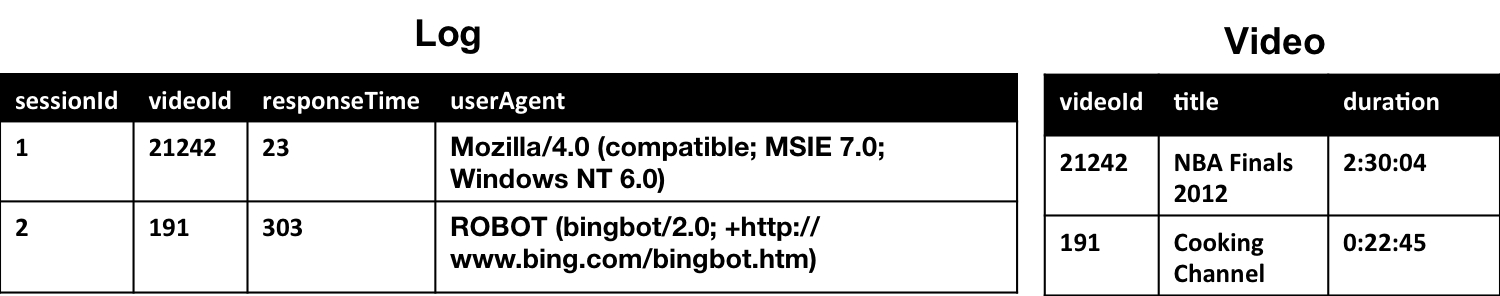
\includegraphics[width=\columnwidth]{figs/sample-clean-example.png}\vspace{-0.25em}
% \caption{A simplified log analysis example dataset. In this dataset, there are two tables: a fact table representing video views and a dimension table representing the videos.\label{example-1}}\vspace{-1em}
%\end{figure}

\iffalse
\subsection{Materialized View Maintenance}\label{subsec-inc}
Views define logical relations which can be queried instead of physical base relations.
MVs are a class of views that are pre-computed and stored (i.e materialized).
Any form of pre-computed, derived data encounters the problem of staleness when the physical base relations update.

One approach to this problem is to recompute the materialized view every time there are updates to the base tables.
However, this approach is very inefficient if updates to the data generally have small or sparse effect on the MV. 
A contrasting approach is incremental view maintenance (IVM), where rows in the MV are incrementally updated based on the updates to the base table.
Incremental maintenance of MVs has been well studied; see \cite{chirkova2011materialized} for a survey of the approaches. 
At a high-level, incremental maintenance algorithms typically consist of the following steps: (1) maintain a cache of insertions and deletions for each physical base table, then using the view definition derive a \emph{change propagation formula} in terms of the set of insertions and deletions, and finally apply the formula to the view.
For a variety of view types, these rules are described in detail in \cite{DBLP:journals/vldb/KochAKNNLS14, DBLP:conf/pods/Koch10}.

%Incremental maintenance may not be efficient in all cases.
%Consider the view that calculates the median \tbl{responseTime} grouped by \tbl{userAgent} on our running example dataset.
%In general, to ensure correctness, the view has to store the entire set of \tbl{responseTime} attributes for each group to allow for incremental maintenance.
%Along the lines of this example, there are cases when recomputation may require less storage of state or even less computation.
%Thus, materialized views are maintained either with incremental maintenance, recomputation, or a mix.

In real-world systems, for large datasets or fast data update rate, it may not always be feasible to maintain MVs immediately. 
Therefore, deferring maintenance (periodically or adaptively) is an alternative and often preferred solution.
The main insight of deferral is to avoid maintaining the view immediately and to schedule an update at a more convenient time.
In deferred maintenance approaches, the user often accepts some degree of staleness for additional flexibility in scheduling.
%SVC offers a data cleaning perspective on this problem, namely, there is a trade-off between the query result accuracy and computation.
By using sampling, we give the user access to a new trade-off space between immediate (or close to immediate, i.e., mini-batch) maintenance and long-periodic maintenance.

%In particular, we highlight a technique called lazy maintenance which applies updates to the view only when a user's query requires a row \cite{zhou2007lazy}.
%While always fresh, both lazy maintenance and immediate maintenance hit a bottleneck when there are rapid updates, and this results increasingly degraded performance if a user wants to query a view.
%The alternative is a periodic strategy, but this means that there is unbounded error on queries between maintenance periods.
%\subsubsection{Practical Considerations}
\fi


\subsection{SampleClean: Fast and Accurate Query Processing on Dirty Data}
In our prior work on the SampleClean project \cite{wang1999sample}, we proposed a framework for scalable data cleaning.
Similar to the accuracy-performance contrast between immediate maintenance and periodic maintenance in the materialized view setting, data cleaning also faces a similar challenge.
Traditionally, data cleaning has explored expensive, up-front cleaning of entire datasets for increased query accuracy, and those who were unwilling to pay the full cleaning cost avoided data cleaning altogether.
We proposed SampleClean to add an additional trade-off to this design space by using sampling.

SampleClean has three parts: (1) sampling, (2) data cleaning, and (3) query result estimation.
First, SampleClean creates a sample of dirty data (which are erroneous, missing, or otherwise corrupted records).
Then, the framework applies a data cleaning procedure to the sample.
Finally, when users query the dataset, the framework uses the clean sample to extrapolate clean query results.
In this work, the main challenge was that data cleaning can potentially change the statistics of a sample and the queries need to compensate for those effects.
In our initial work, SampleClean mainly focused on three common aggregates: \sumfunc, \avgfunc, and \countfunc queries.

The SampleClean project showed that there were two contrasting approaches to query processing on a sample of cleaned data.
We could (1) clean the sample first and then run the query on the sample, or (2) look at the difference between the clean and dirty samples and calculate a correction to correct an existing dirty result. 
Approach (1) is similar to those studied in the Approximate Query Processing (AQP) literature \cite{OlkenR86,AgarwalMPMMS13, joshi2008materialized}; however in cases when data errors were small, we found that the approximation error dominated.
To address this problem, we developed approach (2), which we called \nsc, and we found that \nsc was more accurate in mostly clean datasets as it leverages existing deterministic results leading to reduced approximation error.
In the materialized view setting, we found that \nsc led to more accurate results in our experiments (see Section \ref{exp}). 

%\begin{figure}[t] \vspace{-2em}
%\centering
% 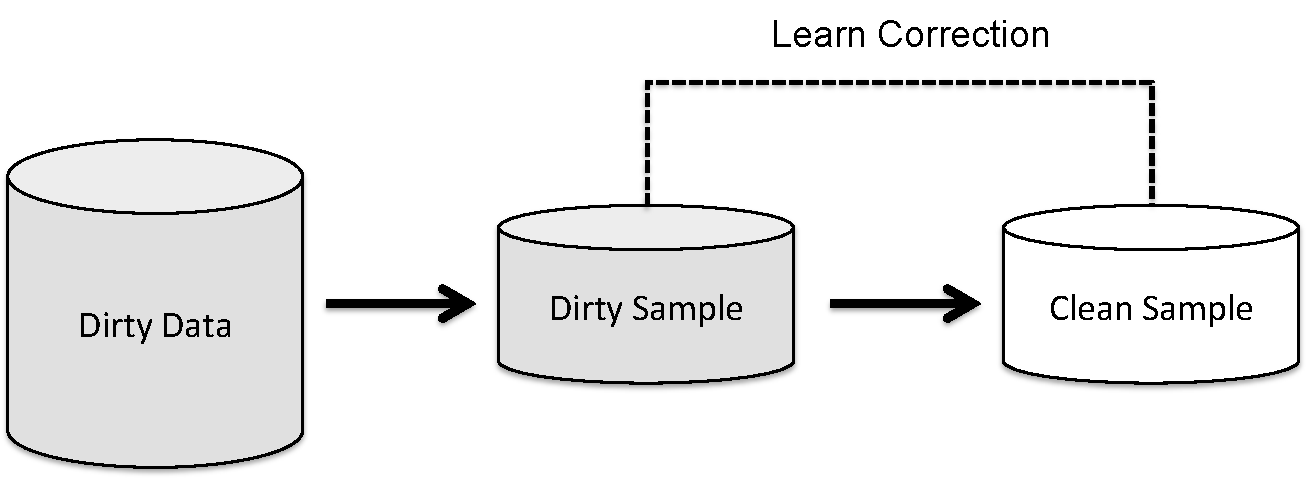
\includegraphics[scale=0.26]{figs/sys-arch2.pdf} \vspace{-.25em}
% \caption{A basic overview of SampleClean. SampleClean uses a random sample of dirty data to learn how a data cleaning algorithm affects queries on the sample. We can then derive a correction to compensate for the dirtiness.\label{sc}}\vspace{-1.75em}
%\end{figure}

\subsection{New Challenges}
%Inspired by SampleClean, SVC samples a stale view, cleans the sample view by restricting the maintenance to just the rows in the sample, and then applies \nsc to correct the results of queries on the stale view.
Applying this data cleaning framework to the materialized view setting leads to some interesting theoretical challenges with new insights for both materialized view maintenance and data cleaning.
%In SampleClean, we simply treated the data cleaning as a black box and did not study how to clean a dirty sample data. 
%However, in SVC, we cannot make such assumption and have to devise efficient data-cleaning techniques to ``clean" a stale sample view. 
Staleness is a new type of data error.
In materialized views, staleness can lead to rows that are missing from the ``dirty" view or conversely need to be deleted. These issues pose new challenges in  query correction. 
We further explore and formalize the class of queries that SVC can support.
We extend the generality of the framework to support queries than the \sumfunc, \avgfunc, and \countfunc which studied before.
Sampling is particularly sensitive to variance in the dataset, and large outliers can significantly reduce query accuracy.
In this work, we give an explicit treatment of outliers records. 

\subsection{Running Example: Log Analysis}
To illustrate our framework in the upcoming sections, we use the following running example which is a 
simplified schema of one of our experimental datasets.
%(Figure~\ref{example-1}).
Imagine, we are querying logs from a video streaming company. 
These logs record visits from users as they happen and grow over time.
We have two tables, \tbl{Log} and \tbl{Video}, with the following schema:

\begin{lstlisting}[mathescape,basicstyle={\scriptsize}]
Log(sessionId$\textrm{,}$ videoId$\textrm{,}$ responseTime$\textrm{,}$ userAgent)
Video(videoId$\textrm{,}$ title$\textrm{,}$ duration)
\end{lstlisting}
These tables are related with a foreign-key relationship between
Log and Video.
Though SVC supports inserts, deletions, and updates, for clarity in our example, we consider insertions
into Log which is cached in a temporary table:

%\reminder{I replace LogInserts with LogIns for saving a line of space. Make sure it is consistent in the whole paper.}
\begin{lstlisting}[mathescape,basicstyle={\scriptsize}]
LogIns(sessionId$\textrm{,}$ videoId$\textrm{,}$ responseTime$\textrm{,}$ userAgent)
\end{lstlisting}





\section{System Overview}\label{sec-arch}
Frequent incremental maintenance of materialized views can be challenging given system resource constraints.
Existing materialized view maintenance techniques lie on a spectrum of accuracy and performance.
Immediate maintenance guarantees that query results on the view will always be accurate, while batch maintenance allows for a higher throughput of updates to the base table.
These two techniques sit at the extremes of the spectrum since they still require that all updates are processed and propagated to the view.

Modeling this problem as a data cleaning problem gives us a new perspective for addressing staleness.
When updates arrive, rows in the materialized view may be either out-of-date or missing altogether; making the view ``dirty".
The challenge is to clean the materialized view by updating the out-of-date rows and inserting the missing rows, however this can be very expensive if there are a large number of updates.
Suppose, we cleaned one dirty row at a time processing only as much of the updates as neccessary to clean the row.
Then, for queries on the view, we get progressively less stale results for a lesser cost.
With this intuition in mind, to ensure that our result is unbiased, we clean a random sample of dirty rows.
For aggregate queries, such as \sumfunc, \countfunc, and \avgfunc, we can then estimate from this sample how the updates change the query results.
From this estimate, we can derive a correction to stale query results.

%Thus, our results are never stale; \reminder{This claim is a little strong. Since we do batch job, is it also possible for us to give stale results?} they have some inaccuracy introduced by the sampling ratio but in expectation they are correct.
%Furthermore, we also prove that this correction term is the optimal linear unbiased estimate for SUM, COUNT, and AVG.

In implementation, our proposed system will work in conjunction with existing maintenance or re-calculation approaches.
We envision the scenario where materialized views are being refreshed periodically eg. nightly.
While maintaining the entire view throughout the day may be infeasible, sampling allows the database to scale maintenance with the performance and resource constraints during the day.
Then, between maintenance periods, we can provide approximately up-to-date query results for aggregation queries.

An additional challenge is that sampling has the potential mask outliers in the updates.
We address this problem by using an ``outlier index" which has been applied in the SAQP setting \cite{chaudhuri2001overcoming}. 

\subsection{System Architecture}
The architecture of our proposed solution is shown in Figure \ref{sys-arch}.
The top of the diagram resembles a typical materialized view maintenance architecture.
However, there are a couple of key additions: (1) as updates arrive we sample the ``update pattern". 
(2) we maintain an outlier index, and (3) we combine the sample and the outlier index to process queries on the stale view.
In this section, we will introduce these three components, which are also explained in much more detail in the following sections.

\begin{figure}[h]
\label{sys-arch}
\centering
 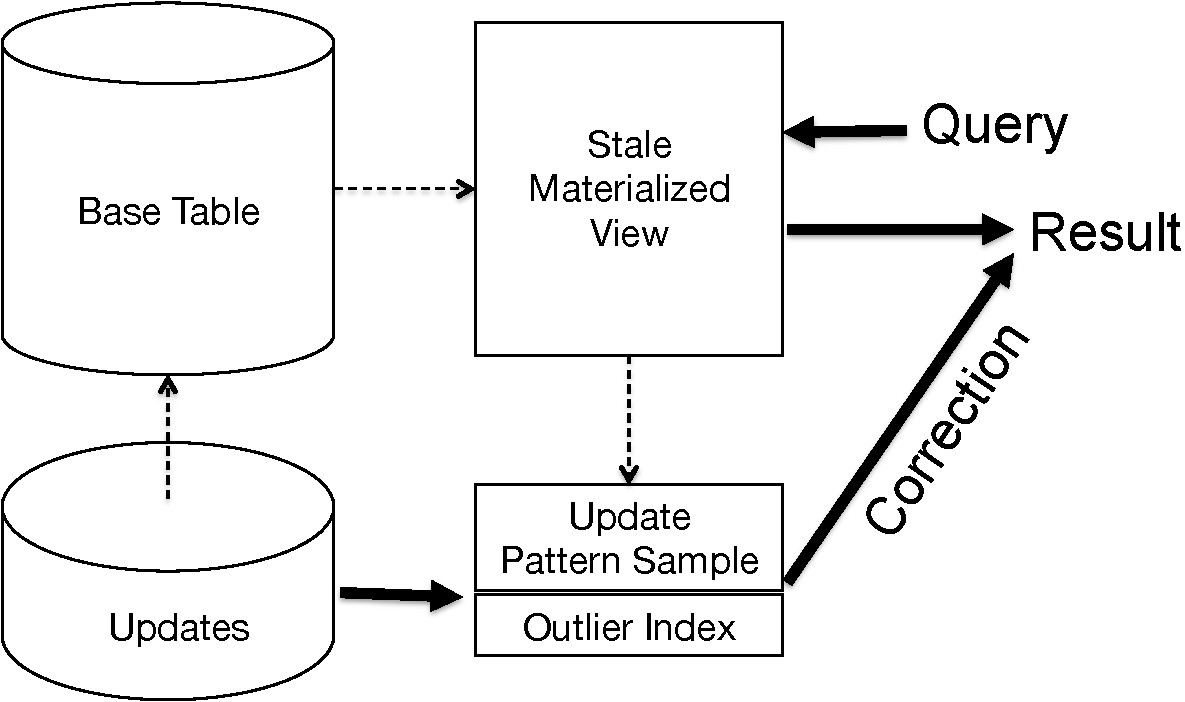
\includegraphics[width=\columnwidth]{figs/sys-arch.pdf}
 \caption{We clean a stale query result by deriving a correction from a sample of up-to-date data. To make this process robust to skewed datasets, we couple sampling with an outlier indexing approach. For aggregation queries, we can guarantee that our results are unbiased and bounded.\reminder{What's the difference between dotted lines and solid lines? Add stale result and update-to-data result into the figure?}}
\end{figure}

\subsubsection{Supported Materialized Views}\label{subsubsec:supported-view}
We will first introduce the taxonomy of materialized views that can benefit from our approach. 
In this paper, we analyze and experiment with three classes of views: Select-Project Views, Foreign-key Join Views, and Aggregation Views.
Our technique can be applied to a broader class of views, please refer to [?] for a full description.
\vspace{1em}

\noindent\textbf{Select-Project Views (\spview): } One type of view that we consider are views generated from Select-Project
expressions of the following form:

\begin{lstlisting}
SELECT [col1,col2,...] 
FROM table 
WHERE condition([col1,col2,...]) 
\end{lstlisting}

\vspace{1em}

\noindent\textbf{Foreign-Key Join Views (\fjview): } As an extension to the Select-Project Views, we can support views derived from a Foreign-Key join:

\begin{lstlisting}
SELECT table1.[col1,col2,...], 
table2.[col1,col2,...]
FROM table1, table2 
WHERE table1.fk = table2.fk 
AND condition([col1,col2,...]) 
\end{lstlisting}

\vspace{1em}

\noindent\textbf{Aggregation Views (\aggview): } We also consider views defined by group-by aggregation queries of the following form:

\begin{lstlisting}
SELECT [f1(col1),f2(col2),...] 
FROM table 
WHERE condition([col1,col2,...]) 
GROUP BY [col1,col2,...]
\end{lstlisting}

\subsubsection{Sampling the Update Pattern}
Given these materialized views, the first challenge is sampling.
We have to sample the updates in a particular way so the sample accurately represents how updates
affect queries on the view. 
The three classes of views require different sampling techniques.
For example, insertions to the base database only result in insertions to Select-Project views.
But, for Aggregation Views, insertions to the base table can also result to updates to existing stale rows.
In Section \ref{sampling}, we describe the sampling algorithm and a cost analysis of how much sampling can reduce maintenance costs.

\subsubsection{Correcting a Query}
Once we have an appropriate sample, we can use information from the sample to correct stale query results.
Suppose, we issue an aggregate query to the stale view.
Then, we scan our sample, and calculate an approximate correction.
The corrected result is in expectation up-to-date and is probabilistically bounded.
Like the sampling, the algorithm to calculate the correction varies between the types of views.
We detail query correction in Section \ref{correction}.

\subsubsection{Outlier Indexing}
We are often interested in records that outliers, 
which we define in this work as records with abnormally large attribute values.
Outliers and power-law distributions are a common property in web-scale datasets.
Often the queries of interest involve the outlier records, however sampling does 
have the potential to mask outliers in the updates.
If we have a small sampling ratio, more likely than not, outliers will be missed.

Therefore, we propose coupling sampling with outlier indexing. 
That is, we guarantee that records (or rows in the view derived from those records) 
with abnormally large attribute values are included in the sample.
What is particularly interesting is that these records give information about the distribution 
and can be used to reduce variance in our estimates.
See Section \label{outlier} for details on this component.

\subsubsection{Example Application: Log Analysis}
To illustrate our approach, we use the following running example which is a 
simplified schema of one of our experimental datasets (Figure ?).
Imagine, we are querying logs from a video streaming company. 
These logs record visits from users as they happen and grow over time.
We have two tables: Log and Video, with the following schema:

\begin{lstlisting}[mathescape]
Log(sessionId$\textrm{,}$ videoId$\textrm{,}$ responseTime$\textrm{,}$ userAgent)
Video(videoId$\textrm{,}$ title$\textrm{,}$ duration)
\end{lstlisting}
These tables are related with a foreign-key relationship between
Log and Video, and there is an integrity constraint that every log
record must link to one video in the video table.

\begin{figure}[h] 
\centering
 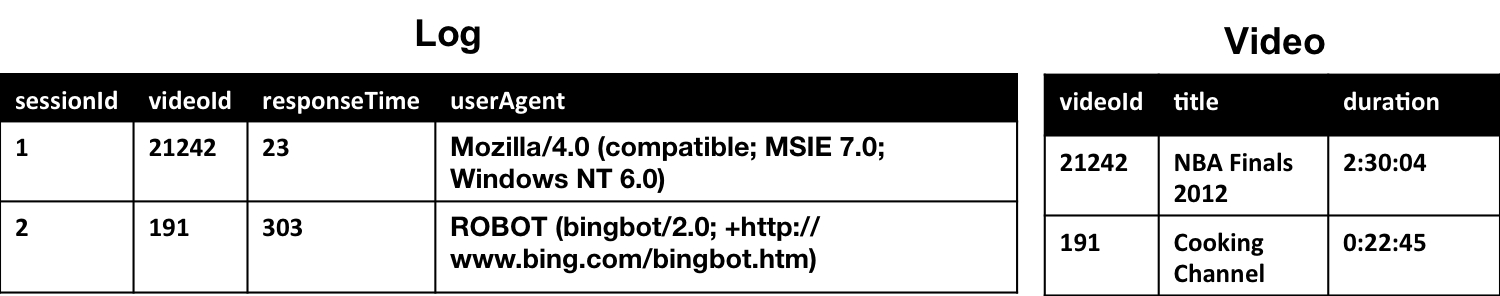
\includegraphics[width=\columnwidth]{figs/sample-clean-example.png}\label{example-1}
 \caption{A simplified log analysis example dataset. In this dataset, there are two tables: a fact table representing video views and a dimension table representing the videos.}
\end{figure}

Consider the following example materialized view \aggview, which stores a result for each video and the maximum time it took for the server to load that video:
\begin{lstlisting} 
SELECT videoId, 
max(responseTime) AS maxResponseTime 
FROM Log 
GROUP BY videoId;
\end{lstlisting}

Suppose, the user creates and materializes this view.
The user wants to know how many videos had a max response time of greater than 100ms.
\begin{lstlisting} 
SELECT COUNT(1)
FROM AggView
WHERE maxResponseTime > 100
\end{lstlisting}
Let us suppose the query result is $15$.
\reminder{The example made the point, but it may need to be polished.}
Since the user queried the table, there have been new logs inserted into to the Log table. 
So materialized aggregation view and the old result of $15$ are now stale.
For example, if our sampling ratio 5\%, our system maintains a sample of this view.
That means for 5\% of the videos (distinct videoID's) we refresh stale maxResponseTime if necessary.
From this sample, we calculate how many new videos changed from a maxResponseTime of less than 100ms to times greater than 100ms; let us suppose this answer is $2$.
Since our sampling ratio is 5\%, we extrapolate that $10$ new videos throughout the view should now be included in the count, resulting in the estimate of $25$.
In contrast, if we had applied SAQP, we would have counted how many videos in the sample had a max response time of greater than 100ms.
In our experiments (Section \ref{exp}), we show that our correction approach compared to SAQP is more accurate when number of updated rows is small compared to the total size of the materialized view.
\section{Efficient Maintenance With Sampling} \label{sampling}
%\reminder{Make sure that we do a good survey on ``sampling from a view" and discuss them in the related work, e.g., [Frank et al., VLDB 86], [Nirkhiwale et al., VLDB 13]}
In the previous section, we formalized the procedure of taking a uniform sample of rows $\hat{S}$, and ``cleaning" it to produce a corresponding uniform sample of the up-to-date view $\hat{S'}$.
This procedure is not unique and there are both efficient and inefficient (i.e., not any easier than updating the entire materialized view) ways to accomplish this. 
For example, a naive solution to derive a sample $\hat{S'}$ is to just apply the maintenance strategy and then sample.
However, this does not make the maintenance of the sample any more efficient.

Ideally, we want to integrate the sampling into the maintenance strategy $\mathcal{M}$ so that expensive operators
need not operate on the full data.
In this section, we discuss how to efficiently derive $\hat{S'}$ and the conditions under which
maintaining $\hat{S'}$ is much cheaper than maintaining the entire view $S'$.

\subsection{Uniform Sampling on Views}
We first discuss some of the difficulties with uniform sampling.
%In this work, we focus on result estimation on uniform samples of views. \reminder{You have already explained uniform sampling in Sec 3.2.}
For a sampling ratio $m$, we call a sample view $\hat{S'}$ a uniform sample of $S'$, under the following condition:
\begin{definition}[Uniform Sample] We say the relation $\hat{S'}$ is a \emph{uniform sample} of $S'$ if
\[\text{(1) } \forall s \in \hat{S'} : s \in S'\text{; (2) }Pr(s_1 \in \hat{S'}) =  Pr(s_2 \in \hat{S'}) = m\]
\end{definition}
A traditional ``coin-flip" sampling algorithm is not suited for this property as it is known that such sampling commutes very poorly with many relational operations such as joins and aggregates \cite{chaudhuri1999random}.
Recall, the view in our example \textsf{countView}. 
Suppose, we sampled from the base relation \tbl{Log}, and then applied the view definition to the sample to form the ``delta view".
The ``delta view" would have a mix of missing videos (\textsf{videoId} is not in the sample) and rows with incomplete aggregates (not all of the videos with \textsf{videoId} are in the sample).
However, this is not what we require since it is not a uniform sample of the rows in the view. 

To get a uniform sample of a view, the main problem is that for every row sampled in the view, our sampling technique needs to include all of the rows in sub-expressions that contribute to its materialization.
Achieving this requires a definition of lineage; traceable, unique identification for rows.

\subsection{Identification With Row Lineage}
\label{lin}
Lineage has been an important tool in the analysis of materialized views \cite{DBLP:journals/vldb/CuiW03} and in approximate query processing \cite{DBLP:conf/sigmod/ZengGMZ14}. %\reminder{Add Kai into acknownledgement for helping us with problem formulation. }
We recursively define a set of consistent primary keys for all nodes in the expression tree:
\begin{definition} [Primary Key]
For every relational expression $R$, we define the primary key of every expression to be:
\begin{itemize}[noitemsep]
\item Base Case: All relations (leaves) must have an attribute $p$ which is designated as a primary key. That uniquely identifies rows.
\item $\sigma_{\phi}(R)$: Primary key of the result is the primary key of R 
\item $\Pi_{(a_1,...,a_k)}(R)$: Primary key of the result is the primary key of R. The primary key must always be included in the projection.
\item $\bowtie_{\phi (r1,r2)}(R_1,R_2)$: The primary key of the result is the union of the primary keys of $R_1$ and $R_2$. 
\item $\gamma_{f,A}(R)$: The primary key of the result is the group by key $A$ (which may be a set of attributes).
\item $R_1 \cup R_2$: Primary key of the result is the primary key of~R
\item $R_1 \cap R_2$: Primary key of the result is the primary key of~R
\item $R_1 - R_2$: Primary key of the result is the primary key of~R
\end{itemize}
\end{definition}
This definition of a primary key for a relational expression, allows us to trace the primary key through the expression tree.
%Our definition of the primary key is also constructive; that is, if an expression has a null primary key then we modify every projection operation to ensure that primary key of the subrelation is never projected out.

\subsection{Hashing Operator}
\label{push}
If we have a deterministic way of mapping a primary key defined in the previous subsection to a sample, we can also ensure that all contributing expressions are also sampled. 
To achieve this we use a hashing procedure.
Let us denote the hashing operator $\eta_{a, m}(R)$. 
For all tuples in R, this operator applies a hash function whose range is $[0,1]$ to primary key $a$ (which may be a set) and selects those records with hash value less than or equal to $m$.
If the hash function is sufficiently uniform, then $h(a) \le m$ samples close to a fraction $m$ of the tuples.
%This definition is without loss of generality for uniform hash function, as if we have a hash function whose range is the set of integers (as implemented in MySQL or Apache Hive) we can take the absolute value and divide by the maximum integer mapping this range back $[0,1]$. 

To achieve the performance benefits of sampling, we push down the hashing operator through the query tree.
The further that we can push $\eta$ down the expression tree, the more operators can benefit from the sampling.
However, it is important to note that for some of the expressions, notably joins, the push down rules are more complex. 
It turns out in general we cannot push down even a deterministic sample through those expressions.
We formalize the push down rules below:
\begin{definition}[Hash Pushdown]
Let $a$ be a primary key of a materialized view. The following rules can be applied to push $\eta_{a, m}(R)$ down the expression tree of the maintenance strategy. 
\begin{itemize}[noitemsep]
\item $\sigma_{\phi}(R)$: Push $\eta$ through the expression.  
\item $\Pi_{p,[a_2,...,a_k]}(R)$: Push $\eta $ through if $a$ is in the projection.
\item $\bowtie_{\phi (r1,r2)}(R_1,R_2)$: Blocks $\eta $ in general. There are special cases below where push down is possible.
\item $\gamma_{f,A}(R)$: Push $\eta $ through if $a$ is in the group by clause $A$.
\item $R_1 \cup R_2$: Push $\eta $ through to both $R_1$ and $R_2$
\item $R_1 \cap R_2$: Push $\eta $ through to both $R_1$ and $R_2$
\item $R_1 - R_2$: Push $\eta $ through to both $R_1$ and $R_2$
\end{itemize}
\end{definition}
In special cases, we can push the hashing operator down through joins. 
Given the hash function $\eta_{a, m}(R)$:

\textbf{Equality Join Key: } If the join is an equality join and $a$ is one of the attributes in the equality join condition $R_1.a = R_2.b$, then $\eta$ can be pushed down to both $R_1$ and $R_2$. On $R_1$ the pushed down operator is $\eta_{a, m}(R_1)$ and on $R_2$ the operator is $\eta_{b, m}(R_2)$.

\textbf{Primary Key Many-to-one: } If we are hashing the primary key of the result of a Foreign-Key join, the push down is possible. We have a join with two relations $R_1$ and $R_2$ and we know that for every $r_1 \in R_1$ there is exactly one $r_2$ in $R_2$ that satisfies the join condition. Based on the lineage rules defined earlier, the primary key is the union of the sets of primary keys of $R_1$ and $R_2$. However, since we know that there is only 1 $r_2$ for every $r_1$, it is equivalent to hash just the primary key of $R_1$. Thus, $a$ in our hash function is the primary key of a Foreign-Key join, then we can push it down to $R_1$, $\eta_{a, m}(R_1)$. 

\textbf{(Semi/Anti)-Join: } Similarly, if we are hashing the primary key of a semi-join, we can always push $\eta$ down $R_1$. For anti-joins we can push $\eta$ down because we can rewrite the node as $R_1 - (R_1 \ltimes R_2) $ and apply the pushdown rules for set difference and Semi-Joins.

\subsection{Corresponding Samples}
We showed that we can optimize a hashed maintenance plan $\eta(\mathcal{M})$ by using push-down rules.
This gives us an expression to maintain a sample of rows in the up-to-date view $S'$.
When the insertion and deletion relations $\{\Delta R_i\} \cup \{\nabla R_i\}$ are not empty, we can use
this expression to propagate changes to our sample.

One benefit of deterministic hashing is that we get the Correspondence Property (Definition \ref{correspondence}) for free.
\begin{proposition}[Hashing Correspondence]
Suppose we have $S$ which is the stale view and $S'$ which is the up-to-date view.
Both these views have the same schema and a primary key $a$.
Let $\eta_{a, m}$ be our hash function that applies the hashing to the primary key $a$.
\[
\hat{S} = \eta_{a, m}(S),\text{ } \hat{S'} = \eta_{a, m}(S')
\]

Then, two samples $\hat{S'}$ and $\hat{S}$ correspond.
\end{proposition}
\begin{proof}[Sketch]
Since the primary keys are key consistent between $\hat{S'}$ and $\hat{S}$, included and excluded rows are preserved by the hashing.
See the extended version for a full proof \cite{technicalReport}.
\iffalse
There are four conditions for correspondence:
\begin{itemize}[noitemsep]
\item 1. For every row $r$ in $\hat{S}$ that required a delete, $r \not\in \hat{S'}$
\item 2. For every row $r$ in $\hat{S}$ that required an update, $r\in \hat{S'}$
\item 3. For every row $r$ in $\hat{S}$  that was unchanged, $r \in \hat{S'}$
\item 4. For every row $r$ in $S$ but not in $\hat{S}$, $r \not\in \hat{S'}$
\end{itemize}
Condition 1 is satisfied since if $r$ is deleted, then $r \not \in S'$ which implies that $r \not\in \hat{S'}$.
Condition 2 and 3 are satisfied since if $r$ is in $\hat{S}$ then it was sampled, and then since the primary key is consistent between $S$ and $S'$ it will also be sampled in $\hat{S'}$.
Condition 4 is just the converse of 2 and 3 so it is satisfied.
\fi
\end{proof}
We will use this property in the Section \ref{correction} to get estimates for queries on the materialized view.

\subsection{Example}
We will illustrate our proposed approach on our example view \textsf{countView} (Figure \ref{exexpr}).
The maintenance strategy of this view is described in the previous section.

Based on the rules described in Section \ref{lin}, the primary key of the view is \textsf{videoId}.
The primary key for base relations \tbl{Log} and \tbl{Video} are \textsf{sessionId} and \textsf{videoId} respectively.
If we move up the tree in Figure \ref{exexpr}, the first expression in the maintenance strategy is a join making the primary key of that expression (\textsf{sessionId}, \textsf{videoId}).
Then, next there is an aggregation which groups by \textsf{videoId} making that the primary key.
This result is an equality the stale view (which has \textsf{videoId} as the primary key) making \textsf{videoId} the primary key of the epression

We can apply our sampling operator to this key, and use the pushdown rules described in Section \ref{push} to efficiently sample the maintenance strategy.
In Figure \ref{exexpr2}, we illustrate the pushdown process.
The the first operator we see in the expression tree is a projection that increments the \textsf{visitCount} in the view, and this allows
for push down since \textsf{videoId} is in the projection.
The second expression is a hash of the equality join key which merges the aggregate from the ``delta view" to the old view allowing us to push down on both branches of the tree.
On the left side, we reach the the stale view so we stop.
Since the stale view does not change, we can calculate the sample of the stale view once (eg. during periodic maintenance). 
On the right side, we reach the aggregate query (count) and since \textsf{videoId} is in group by clause, we can push down the sampling.
Then, we reach another point where we hash the equality join key allowing us to push down the sampling to the relation \tbl{LogIns} and \tbl{Video}.

\begin{figure}[t] \vspace{-2em}
\centering
 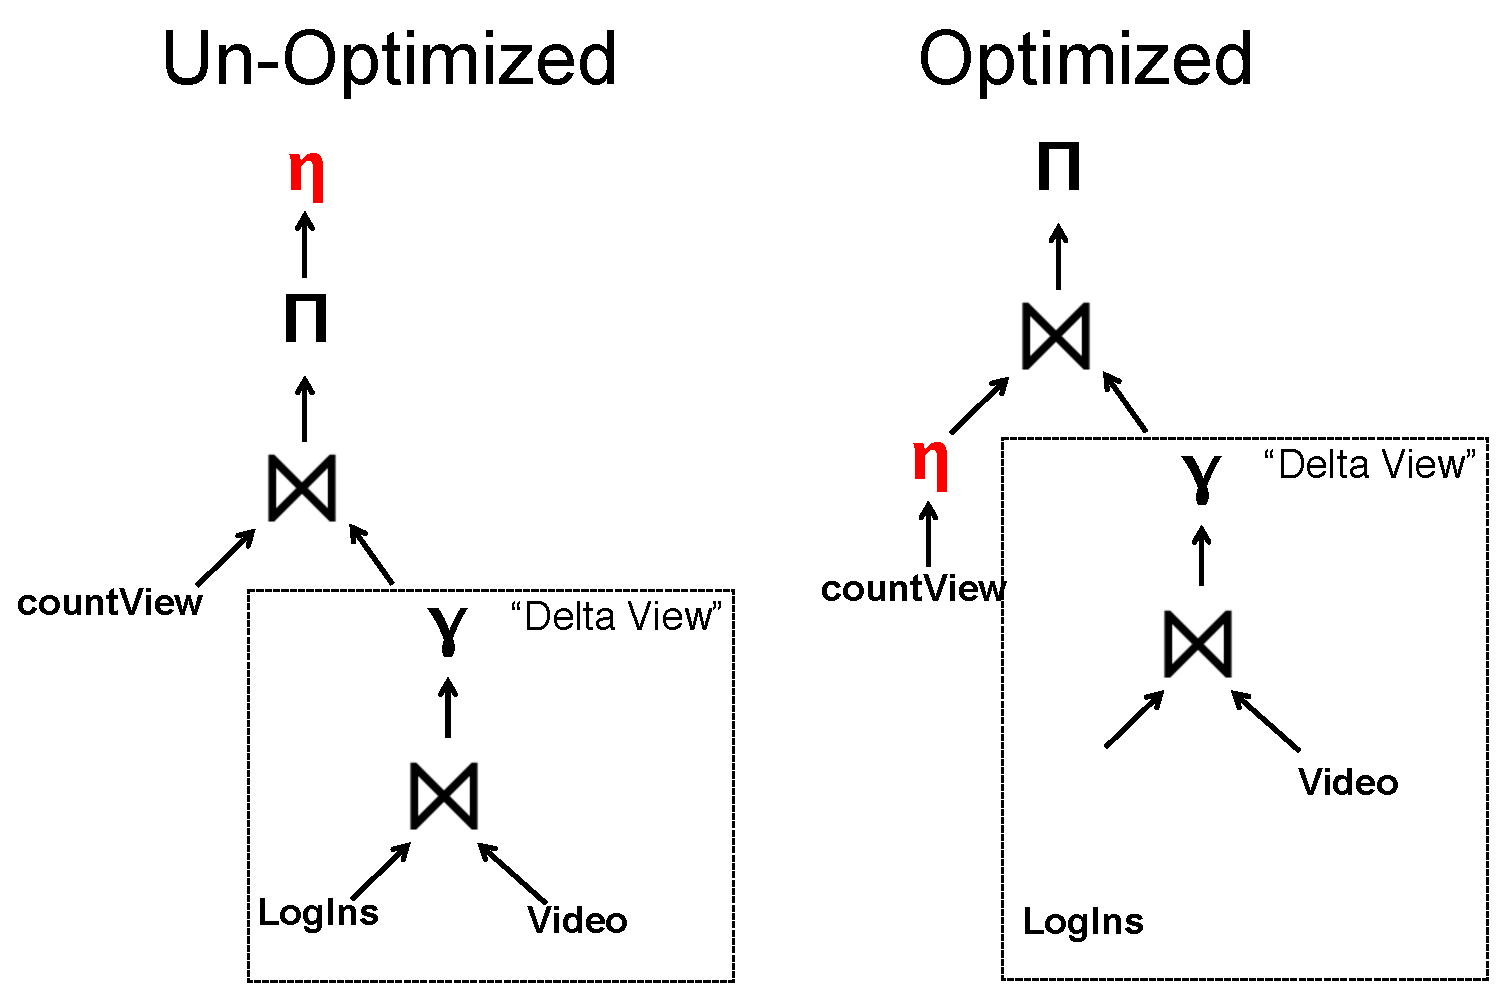
\includegraphics[scale=0.20]{figs/example_expression_tree_2.pdf} \vspace{-.25em}
 \caption{Applying the rules described in Section \ref{push}, we illustrate how to optimize the sampling of our example maintenance strategy.  \label{exexpr2}}\vspace{-1.75em}
\end{figure}

In terms of increased efficiency, since both the aggregation and joins are ``above" the sampling operator, they require less computation and less memory.



\section{Query Result Estimation}
\label{correction}
%In the previous section, we discussed how to efficiently maintain a sample of a materialized view by applying the hashing operator to the maintenance strategy.
%The result of the previous section is a cleaned sampled materialized view $\hat{S'}$.
\svc returns two corresponding samples, $\widehat{S}$ and $\widehat{S}'$.
$\widehat{S}$ is a ``dirty" sample (sample of the stale view) and $\widehat{S}'$ is a ``clean" sample (sample of the up-to-date view).
In this section, we first discuss how to estimate query results using the two corresponding samples. 
Then, we discuss the bounds and guarantees on different classes of aggregate queries.

%Our data cleaning perspective allows us to look at each dirty row in an MV and what cleaning was applied to clean it (insert, delete, or update).
%We can use this analysis to calculate corrections that compensate for the effect of staleness of aggregate queries.
%The intuition is to take a point-wise difference of $\hat{S'}$ and $\hat{S}$ which is challenging in the presence of missing data.
%This gives us a uniform sample of the differences between the stale view and a hypothetical up-to-date view, and allows us to test how query results can be affected by the updates.
%\reminder{The following text is not consistent with the structure of the section.}
%We first present our extensions to the existing SampleClean queries: \sumfunc, \countfunc, and \avgfunc.
%Then, we discuss how to extend this framework to other aggregate functions.
%We also show how SampleClean can work with biased estimates as well and what statistical tools we can use to bound these estimates.
%Next, we discuss selection queries and how SampleClean can give limited support to these.
%We summarize these results in Table \ref{table:nonlin}, where we list common aggregation queries and describe 
%how \svc estimates their results. 
%Finally, we analyze the cost of query correction.




\subsection{Result Estimation}\label{re}
Suppose, we have an aggregate query $q$ of the following form:
\begin{lstlisting} [mathescape]
$\;\;\;\;$q(View) := SELECT f(attr) FROM View WHERE cond(*)
\end{lstlisting}
We quantify the staleness $c$ of the aggregate query result as the difference
between the query applied to the stale view $S$ compared to the up-to-date view $S'$:
\[
q(S') = q(S) + c
\]
The objective of this work is to estimate $q(S')$.
In the Approximate Query Processing (AQP) literature, sample-based estimates have been well studied \cite{OlkenR86, AgarwalMPMMS13}.
This inspires our first estimation algorithm, \svcnospace+AQP, which uses \svc to materialize a sample view and an AQP-style
result estimation technique.

\vspace{0.25em}

\noindent\textbf{SVC+AQP: }  Given a clean sample view $\widehat{S}'$, the query $q$, and a scaling factor $s$. 
We apply the query to the sample and scale it by $s$:
\[
q(S') \approx s \cdot q(\widehat{S}')
\]
For example, for the \sumfunc and \countfunc the scaling factor is $\frac{1}{m}$. For the \avgfunc the scaling factor is 1.
Determining these scaling factors is discussed in in the AQP literature \cite{OlkenR86, AgarwalMPMMS13}.

\svcnospace+AQP returns what we call a direct estimate of $q(S')$.
We could, however, try to estimate $c$ instead.
Since we have the stale view $S$, we could run the query $q$ on the full stale view and 
estimate the difference $c$ using the samples $\widehat{S}$ and $\widehat{S}'$.
We call this approach \svcnospace+CORR, which represents calculating a correction to $q(S)$ instead of a direct estimate.

\vspace{0.25em}

\noindent\textbf{SVC+CORR: } Given a clean sample $\widehat{S}'$, its corresponding dirty sample $\widehat{S}$, a query q, and a scaling factor $s$:
\begin{enumerate}[noitemsep]
\item Apply \svcnospace+AQP to $\widehat{S}'$:
\[ r_{est\_fresh} = s \cdot q(\widehat{S}') \] 
\item Apply \svcnospace+AQP to $\widehat{S}$:
\[ r_{est\_stale} = s \cdot q(\widehat{S}) \] 
\item Apply q to the full stale view:
\[ r_{stale} = q(S) \]
\item Take the difference between (1) and (2) and add it to (3):
\[
q(S') \approx r_{stale} + (r_{est\_fresh} - r_{est\_stale})
\]
\end{enumerate}

A commonly studied property in the AQP liture is unbiasedness.
An unbiased result estimate means that average value of the estimate over all possible samples is $q(S')$.
We can prove that if \svcnospace+AQP is unbiased (there is an AQP method that gives an unbiased result) then \svcnospace+CORR also gives unbiased results.
\begin{lemma}\label{lemma:unbiased}
If there exists an unbiased sample estimator for q(S') then there exists an unbiased sample estimator for c.
\end{lemma}
\begin{proof}[Sketch] 
Suppose, we have an unbiased sample estimator $e_q$ of $q$. 
Then, it follows that \[\mathbb{E}\big[e_q(\hat{S'})\big] = q(S')\]
If we substitute in this expression:
$c = \mathbb{E}\big[e_q(\hat{S'})\big] -q(s) $
Applying the linearity of expectation:
\[ c = \mathbb{E}\big[e_q(\hat{S'}) - q(s)\big] \]
\end{proof}
Some queries do not have unbiased sample estimators, but the bias of their sample estimators can be bounded. Example queries include: \medfunc, \percfunc.
A corollary to the previous lemma, is that if we can bound the bias for our estimator then we can achieve a bounded bias for $c$ as well.
%\begin{corollary}
%If there exists a bounded bias sample estimator for $q$ then there exists a bounded bias sample estimator for $c$.
%\end{corollary}


\begin{example}
We can formalize our earlier example query in Section \ref{infexample} in terms of SVC+CORR and SVC+AQP.
Let us suppose the initial query result is $45$.
There now have been new log records inserted into the Log table making the old result stale, and suppose we are working with a sampling ratio of 5\%.
For SVC+AQP, we count the number of videos in the sample that currently have counts greater than 100 and scale that result by 20.
For SVC+CORR, suppose 2 videos have changed their counts from less than 100 to greater than 100.
From this sample, we calculate how many new videos changed from less than 100 views to times greater than 100; let us suppose this answer is $2$.
We extrapolate that $40$ new videos throughout the view should now be included in the count.
This means that we should correct the old result by $40$ resulting in the estimate of $45+40 = 85$.
\end{example}

\subsection{Estimate Accuracy}
To analyze the estimate accuracy, we taxonomize common SQL aggregate queries into different \emph{estimator families}.
For example, \sumfunc, \countfunc, and \avgfunc can all be written as sample means.
\sumfunc is the sample mean scaled by the relation size and \countfunc is the mean of the indicator function scaled by the relation size.
There are some key properties of interest within different estimator families: unbiasedness, existence analtyic confidence intervals, and optimality.
\svcnospace+AQP and \svcnospace+CORR inherit the properties of the estimator family.

Table \ref{estimators} describes these families and their properties for common queries.
Sample mean family of estimators (\sumfunc, \countfunc, and \avgfunc) has analytic solutions and has been the focus of other approximate query processing works \cite{OlkenR86, wang1999sample}, we analyze this family in detail.
The general case can only be bounded empirically which is more challenging.

\begin{table}\scriptsize
\begin{tabular}{ l l l l}
  SQL Query & Estimator Family & Unbiased & Estimate Variance \\ \hline
  \avgfunc, \sumfunc, \countfunc & Sample Mean & Yes & Optimal \\
  \stdfunc, \varfunc & Sample Variance & Yes & Optimal \\
  \medfunc, \percfunc & Sample Ranking & Bounded & Suboptimal \\
  \maxfunc, \minfunc & Sample Extrema & Unbounded & Suboptimal \\
\end{tabular}
\caption{SQL queries and the properties of their statistical estimation family. \label{estimators}}
\end{table}

\subsubsection{Confidence Intervals For Sample Means}
Now we will discuss bounding our estimates in confidence intervals for \sumfunc, \countfunc, and \avgfunc, which can be
estimated with ``sample mean" estimators.
Sample means for uniform random samples (also called sampling without replacement) converge to the population mean by the Central Limit Theorem (CLT).
Let $\hat{\mu}$ be a sample mean calculated from $k$ samples, $\sigma^2$ be the variance of the sample, and $\mu$ be the population mean. 
Then, the error in the estimate is normally distributed\footnote{We can include a finite population correction if our relation size is small $\frac{N-k}{N-1}$.}:
\[
(\mu - \hat{\mu}) \sim N(0,\frac{\sigma^2}{k})
\]
Therefore, the confidence interval is given by:
\[
\hat{\mu} \pm \gamma \frac{\sigma^2}{k}
\]
where $\gamma$ is the Gaussian tail probability value (eg. 1.96 for 95\%, 2.57 for 99\%).

Next, we discuss how to calculate this confidence interval in SQL for SVC+AQP.
The first step is a query rewriting step where we express the query on the view in terms of a \textsf{case} statement (1 if true, 0 if false)
instead of a predicate.
Let \emph{attr} be the aggregate attribute and $m$ be the sampling ratio. 
We define an intermediate result $trans$ which is a table of transformed rows with the first column the 
primary key and the second column defined in terms of a \texttt{case} statement and scaling.
For \sumfunc:
\begin{lstlisting}[mathescape,basicstyle={\scriptsize}]
trans(sample):= SELECT pk, 
1.0/m $\cdot$ attr $\cdot$ cond(*) as trans_attr
FROM sample 
\end{lstlisting} 
For \avgfunc since there is no scaling we do not need to re-write:
\begin{lstlisting}[mathescape,basicstyle={\scriptsize}]
trans(sample) := SELECT pk, attr as trans_attr 
WHERE cond(*) FROM sample
\end{lstlisting}
For \countfunc:
\begin{lstlisting}[mathescape,basicstyle={\scriptsize}]
trans(sample) := SELECT pk, 1.0/m $\cdot$ cond(*) as trans_attr
FROM sample
\end{lstlisting}

\vspace{0.25em}

\noindent\textbf{SVC+AQP: } The confidence interval on this result is defined 
as:
\begin{lstlisting}[mathescape,basicstyle={\scriptsize}]
SELECT $\gamma\cdot$stdev(trans_attr)/sqrt(count(1)) FROM trans
\end{lstlisting}

\vspace{0.25em}

To calculate the confidence intervals for \svcnospace+CORR we have to look at the statistics of $c$ the difference i.e. $c = q(S) - q(S')$ from a sample.
For queries that can be estimated with a sample mean, we can use the associativity of addition and subtraction to rewrite this as:
\[c = q(S - S')\]
Where $-$ is the row-by-row difference between $S$ and $S'$.
The problem is that some rows in $\widehat{S}$ do not exist in $\widehat{S}'$ and vice versa. 
Thus, we have define the following null-handling semantics with a subtraction operator we call $\dot{-}$.
\begin{definition}[Correspondence Subtract] Given an aggregate query, and two corresponding relations $R_1$ and $R_2$ with the schema $(a_1, a_2, ...)$ where $a_1$ is the primary key for $R_1$ and $R_2$, and $a_2$ is the aggregation attribute for the query. 
$\dot{-}$ is defined as a projection of the full outer join on equality of $R_1.a_1 = R_2.a_1$: \[ \Pi_{R_1.a_2 - R_2.a_2} ( R_1 \fullouterjoin R_2 ) \]
Null values $\emptyset$ are represented as~zero.
\end{definition}
Using this operator, we can define a new intermediate result $diff$:
\[diff := trans(\widehat{S}') \dot{-} trans(\widehat{S}) \]

\vspace{0.35em}\noindent\textbf{SVC+CORR: } Then, as in \svcnospace+AQP, we bound the result using the CLT:
\begin{lstlisting}[mathescape,basicstyle={\scriptsize}]
SELECT $\gamma\cdot$stdev(trans_attr)/sqrt(count(1)) FROM diff
\end{lstlisting}

\subsubsection{AQP vs. CORR For Sample Means}
In terms of these bounds, we can analyze how \svcnospace+AQP compares to \svcnospace+CORR for a fixed sample size $k$.
\sloppy
\svcnospace+AQP gives an estimate that is proportional to the variance of the clean sample view: 
$\frac{\sigma_{S'}^2}{k}$.
\svcnospace+CORR to the variance of the \emph{differences}: 
$\frac{\sigma_{c}^2}{k}$.
Since the change is the difference between the stale and up-to-date view, this can be rewritten as
\[\frac{\sigma_{S}^2 + \sigma_{S'}^2 - 2cov(S,S')}{k}\]
Therefore, a correction will have less variance when:
\[\sigma_{S}^2 \le 2cov(S,S')\]

As we saw in the previous section, correspondence correlates the samples.
If the difference is small, i.e. $S$ is nearly identical to $S'$,then $cov(S,S')~\approx~\sigma_{S}^2$. 
This result also shows that there is a point when updates to the stale MV are significant enough that direct estimates are more accurate.
When we cross the break-even point we can switch from using \svcnospace+CORR to \svcnospace+AQP.
%An intersting implication of this break-even point is it gives us a bound on the approximation error no matter how significant the staleness is.
\svcnospace+AQP does not depend on $cov(S,S')$ which is a measure of how much the data has changed.
Thus, we guarantee an approximation error of at most $\frac{\sigma_{S'}^2}{k}$.
In our experiments (Figure \ref{exp-1-total}(b)), we evaluate this break even point empirically. 

\subsubsection{Selectivity For Sample Means}
Let $p$ be the selectivity of the query; that is, a fraction $p$ records from the relation satisfy the predicate.
For these queries, we can model selectivity as a reduction of effective sample size making the
estimate variance: $O(\frac{1}{k*p})$.
Thus, the confidence interval's size is scaled up by $\frac{1}{\sqrt{p}}$.
Just like there is a tradeoff between accuracy and maintenance cost, for a fixed accuracy 
there is also a tradeoff between answering more selective queries and maintenance cost.

\subsubsection{Optimality For Sample Means}
Optimality in unbiased estimation theory is defined in terms of the variance of the estimate \cite{cox1979theoretical}.
\begin{proposition}
An estimator is called a minimum variance unbiased estimator (MVUE) if it is unbiased and the variance of the estimate is less than or equal to that of any other unbiased estimate.
\end{proposition}

A sampled relation $R$ defines a discrete distribution.
It is important to note that this distribution is different from the data generating distribution, since even if $R$ has continuous valued attributes
$R$ still defines a discrete distribution.
Our population is finite and we take a finite sample thus every sample takes on only a discrete set of values.
In the general case, this distribution is only described by the set of all of its values (i.e no smaller parametrized representation).
In this setting, the sample mean is an MVUE.
In other words, if we make no assumptions about the underlying distribution of values in $R$, SVC+AQP and SVC+CORR are optimal for their respective estimates ($q(S')$ and $c$).
Since they estimate different variables, even with optimality SVC+CORR might be more accurate than SVC+AQP and vice versa. 

However, if we do know more about the distribution, this optimality is not true in general.
The intuitive problem is that if there are a small number of parameters that completely describe the discrete distribution there might be 
a way to reconstruct the distribution from those parameters rather than estimating the mean.
As a simple counter example, if we knew our attributes were exactly on a line, a sample size of two is sufficient to answer any aggregate query.
However, even for many discrete parametric distributions, the sample mean estimators are MVUEs, eg. poisson, bernouilli, binomial, hypergeometric.
It is often difficult and unknown in many cases to derive an MVUE other than a sample mean.
Our approach is valid for any choice of estimator, even though we do the analysis for sample mean estimators.

\subsubsection{General Estimators}
The theory for bounding general estimators outside of the sample mean family is more complex.
We may not get analytic confidence intervals on our results, nor is it guaranteed that our estimates are optimal.
In AQP, the commonly used technique is called a statistical bootstrap \cite{AgarwalMPMMS13} to empirically bound the results.
In this approach, we repeatedly subsample with replacement from our sample and apply the query to the sample.
This gives us a technique to bound SVC+AQP the details of which can be found in \cite{AgarwalMPMMS13, agarwalknowing, DBLP:conf/sigmod/ZengGMZ14}. 
For SVC+CORR, we have to propose a new variant of bootstrap to bound the estimate of $c$.
In this variant, repeatedly estimate $c$ from subsamples and build an empirical distribution for $c$.

\vspace{0.35em}

\noindent\textbf{SVC+CORR: } To use bootstrap to find a 95\% confidence interval:
\begin{enumerate}[noitemsep]
\item Subsample $\widehat{S}_{sub}'$ and $\widehat{S}_{sub}$ with replacement from $\widehat{S}'$ and $\widehat{S}$ respectively
\item Apply SVC+AQP to $\widehat{S}_{sub}'$ and $\widehat{S}_{sub}$
\item Record the difference $s\cdot(q(\widehat{S}_{sub}')-q(\widehat{S}_{sub}))$
\item Return to 1, for k iterations.
\item Return the $100-\alpha$\% and the $\alpha$\% percentile of the distribution of results.
\end{enumerate}

%Bootstrap is known to be computationally intensive.
%There has been recent research in using techniques such as Poissonized resampling \cite{agarwalknowing}, analytical bootstrap\cite{DBLP:conf/sigmod/ZengGMZ14}, and bagging \cite{DBLP:conf/kdd/KleinerTASJ13} to make this algorithm better suited for latency-sensitive query processing application.
%Furthermore, bootstrap will only work when estimator satisfies some differentiability conditions \cite{agarwalknowing}.
%Refer to the extended technical report for the details on the bootstrap procedure \cite{technicalReport}.
\iffalse
\subsubsection{MIN and MAX}
\minfunc and \maxfunc fall into their own category since this is a canonical case where bootstrap fails.
We devise an estimation procedure that corrects these queries.
However, we can only achieve bound that has a slightly different interpretation than the confidence intervals seen before.
We can calculate the probability that a larger (or smaller) element exists in the unsampled view.
%Refer to the extended technical report for the details on \minfunc and \maxfunc \cite{technicalReport}.

We devise the following correction estimate for \maxfunc: (1) For all rows in both $S$ and $S'$, calculate the row-by-row difference, (2) let $c$ be the max difference, and (3) add $c$ to the max of the stale view.

We can give weak bounds on the results using Cantelli's Inequality.
If $X$ is a random variable with mean $\mu_x$ and variance $var(X)$, then the probability that $X$ is larger than a constant $\epsilon$ 
\[
\mathbb{P}(X \ge \epsilon + \mu_x ) \le \frac{var(X)}{var(X) + \epsilon^2}
\]
Therefore, if we set $\epsilon$ to be the difference between max value estimate and the average value, we can calculate the probability that we will see a higher value. 

The same estimator can be modified for \minfunc, with a corresponding bound:
\[
\mathbb{P}(X \le \mu_x - a )) \le \frac{var(x)}{var(x) + a^2}
\]
This bound has a slightly different interpretation than the confidence intervals seen before.
This gives the probability that a larger (or smaller) element exists in the unsampled view.


\vspace{-.25em}
\subsection{Select Queries}
In \svc, we also explore how to extend this correction procedure to Select queries.
Suppose, we have a Select query with a predicate:
\begin{lstlisting} [mathescape]
SELECT $*$ FROM View WHERE Condition(A);
\end{lstlisting}

We first run the Select query on the stale view, and this returns a set of rows.
This result has three types of data error: rows that are missing, rows that are falsely included, and rows whose values are incorrect.

As in the \sumfunc, \countfunc, and \avgfunc query case, we can apply the query to the sample of the up-to-date view.
From this sample, using our lineage defined earlier, we can quickly identify which rows were added, updated, and deleted.
For the updated rows in the sample, we overwrite the out-of-date rows in the stale query result.
For the new rows, we take a union of the sampled selection and the updated stale selection.
For the missing rows, we remove them from the stale selection.
To quantify the approximation error, we can rewrite the Select query as \countfunc to get an estimate of number of rows that were updated, added, or deleted (thus three ``confidence'' intervals). 
\fi


\iffalse
\subsection{Bounded Bias Aggregates}
Some queries do not have unbiased sample estimators, but the bias of their sample estimators can be bounded. Example queries include: \medfunc, \percfunc.

A corollary to the previous lemma, is that if we can bound the bias for our estimator then we can achieve a bounded bias for $c$ as well.
\begin{corollary}
If there exists a bounded bias sample estimator for $q$ then there exists a bounded bias sample estimator for $c$.
\end{corollary}

What this means for a user is that the error bars are asymmetric with increased error in the direction of the bias (often in the direction of skew in the dataset).
Functionally, we can apply the same technique discussed in the previous section for these queries and apply the bootstrap to bound the results. 
\fi

\iffalse 

\subsection{Query Execution Cost}
It is true that \svc adds to the query execution time by issuing a correction. 
However, this correction is only calculated on a sample and thus is small compared to the query execution time over the entire old view.
In our experiments, we show that the overheads are small in comparison to the execution time over the entire old view and the savings from only maintaining a sample (Section \ref{exp-datacube}).
\fi
\vspace{-.5em}
\section{Outlier Indexing}\label{outlier}
Sampling is known to be sensitive to outliers \cite{clauset2009power, chaudhuri2001overcoming}.
Power-laws and other long-tailed distributions are common in practice \cite{clauset2009power}.
We address this problem using a technique called outlier indexing which has been applied in AQP \cite{chaudhuri2001overcoming}.
The basic idea is that we create an index of outlier records (records whose attributes deviate from the mean value greatly) and ensure that these records are included in the sample.
The intuition is that these records greatly increase the variance of the data. 
Furthermore, since they are likely rare the probability of sampling them is low leading to wildly varying estimates.  
However, as this has not been explored in the materialized view setting there are new challenges in using this index for improved result accuracy.

\subsection{Indices on the Base Relations}
In \cite{chaudhuri2001overcoming}, the authors applied outlier indexing to improve the accuracy of AQP.
We apply a similar technique, however, their problem setting is different in a few ways.
First, in the AQP setting, queries are issued to base relations.
In our problem, we issue queries to materialized views.
We need to define how to propagate information from an outlier index on the base relation to a materialized view.

The first step is that the user selects an attribute of any base relation to index and specifies a threshold $t$ and a size limit $k$.
In a single pass of updates (without maintaining the view), the index is built storing references to the records with attributes greater than $t$.
If the size limit is reached, the incoming record is compared to the smallest indexed record and if it is greater then we evict the smallest record.
The same approach can be extended to attributes that have tails in both directions by making the threshold $t$ a range, which takes the highest and the lowest values.
However, in this section, we present the technique as a threshold for clarity.

There are many approaches to select a threshold.
We can use prior information from the base table, a calculation which can be done in the background during the periodic maintenance cycles.
If our size limit is $k$, for a given attribute we can select the the top-k records with that attributes.
Then, we can use that top-k list to set a threshold for our index. 
Then, the attribute value of the lowest record becomes the threshold $t$.
Alternatively, we can calculate the variance of the attribute and set the threshold to represent $c$ standard deviations above the mean.

This threshold can be adaptively set at each maintenance period to include more or less outliers.
The caveat is that the outlier index should not be too expensive to calculate nor should it be too large as it negates the performance benefits of sampling.  
The query processing approach that we propose in the following sub-sections is agnostic to how we choose this threshold.
In fact, our approach allows us to incorporate any deterministic subset into our sample-based correction calculations.

\subsection{Adding Outliers to the Sample}
%Given this index, the next question is how we can use this information in our materialized views.
We ensure that any row in a materialized view that is derived from an indexed record is guaranteed to be in the sample.
This problem is sort of an inverse to the efficient sampling problem studied in Section~\ref{sampling}.
We need to propagate the indices upwards through the expression tree.

%The next challenge is the outlier index must not require any additional effort to materialize.
We add the condition that the only eligible indices are ones on base relations that are being sampled (i.e., we can push the hash operator down to that relation).
Therefore, in the same iteration as sampling, we can also test the index threshold and add records to the outlier index. 
We formalize the propagation property recursively. 
Every relation can have an outlier index which is a set of attributes and a set of records that exceed the threshold value on those attributes.

The main idea is to treat the indexed records as a sub-relation that gets propagated upwards with the maintenance strategy.
\begin{definition}[outlier index pushup]
Define an outlier index to be a tuple of a set of indexed attributes, and a set of records $(I,O)$. The outlier index propagates upwards with the following rules: 
\begin{itemize}[noitemsep]
\item Base Relations: Outlier indices on base relations are pushed up only if that relation is being sampled, i.e., if the sampling operator can be pushed down to that relation.
\item $\sigma_{\phi}(R)$: Push up with a new outlier index and apply the selection to the outliers $(I,\sigma_{\phi}(O))$ 
\item $\Pi_{(a_1,...,a_k)}(R)$: Push upwards with new outlier index $(I \cap (a_1,...,a_k), O)$.
\item $\bowtie_{\phi (r1,r2)}(R_1,R_2)$: Push upwards with new outlier index $(I_{1} \cup I_{2}, O_1 \bowtie O_2)$. 
\item $\gamma_{f,A}(R)$: For group-by aggregates, we set $I$ to be the aggregation attribute. For the outlier index, we do the following steps. (1) Apply the aggregation to the outlier index $\gamma_{f,A}(O)$, (2) for all distinct $A$ in $O$ select the row in $\gamma_{f,A}(R)$ with the same $A$, and (3) this selection is the new set of outliers $O$. 
\item $R_1 \cup R_2$: Push up with a new outlier index $(I_1 \cap I_2, O_1 \cup O_2)$. The set of index attributes is combined with an intersection to avoid missed outliers.
\item $R_1 \cap R_2$: Push up with a new outlier index $(I_1 \cap I_2, O_1 \cap O_2)$.
\item $R_1 - R_2$: Push up with a new outlier index $(I_1 \cup I_2, O_1 - O_2)$.
\end{itemize}
\end{definition}

For all outlier indices that can propagate to the view (i.e., the top of the tree), we get a final set $O$ of records. 
Given these rules, $O$ is, in fact, a subset of our materialized view $S'$.
Thus, our query processing can take advantage of the theory described in the previous section to incorporate the set $O$ into our results.
We implement the outlier index as an additional attribute on our sample with a boolean flag true or false if it is an outlier indexed record.
If a row is contained both in the sample and the outlier index, the outlier index takes precedence.
This ensures that we do not double count the outliers.

\subsection{Query Processing}\label{oqp} 
For result estimation, we can think of our sample $\hat{S'}$ and our outlier index $O$ as two distinct parts.
Since $O \subset S'$, and we give membership in our outlier index precedence, our sample is actually a sample restricted to the set $\widehat{(S'-O)}$. 
The outlier index has two uses: (1) we can query all the rows that correspond to outlier rows, 
and (2) we can improve the accuracy of our \emph{aggregation} queries.
To query the outlier rows, we can select all of the rows in the materialized view that are flagged as outliers, and these rows are guaranteed to be up-to-date.

For (2), we can also incorporate the outliers into our correction estimates.  
For a given query, let $c_{reg}$ be the correction calculated on $\widehat{(S'-O)}$ using the technique proposed in the previous section and adjusting the sampling ratio $m$ to account for outliers removed from the sample.
We can also apply the technique to the outlier set $O$ since this set is deterministic the sampling ratio for this set is $m=1$, and we call this result $c_{out}$.
Let $N$ be the count of records that satisfy the query's condition and $l$ be the number of outliers that satisfy the condition.
Then, we can merge these two corrections in the following way:
$
 v = \frac{N-l}{N}c_{reg} + \frac{l}{N}c_{out}
$.

For the queries in the previous section that are unbiased, this approach preserves unbiasedness.
Since we are averaging two unbiased estimates $c_{reg}$ and $c_{out}$, the linearity of the expectation operator preserves this property.
Furthermore, since $c_{out}$ is deterministic (and in fact its bias/variance is 0), $c_{reg}$ and $c_{out}$ are uncorrelated making the bounds described in the previous section applicable as well.

\subsection{Example}
Suppose, we want to use outlier indexing to process queries on \tbl{visitView}.
We chose an attribute in the base data to index, for example \texttt{duration}.
We can set an threshold of 1.5 hours (e.g, indexes all of the movies served by the system).
This materializes the entire set of rows whose duration is longer than 1.5 hours.

Returning to the example query from the previous section:
\begin{lstlisting}[basicstyle={\scriptsize}]
SELECT COUNT(1) FROM visitView 
WHERE visitCount > 100;
\end{lstlisting}
We run SVC+AQP and SVC+CORR on the set of rows with durations longer than 1.5 hours.
Then we use the update rule in Section \ref{oqp} to update the result based on the number of records in the index and the total size of the view.

%sum of uncorrelated unbiased estimates since one is deterministic.

%See \cite{chaudhuri2001overcoming} for additional query processing details.
%\section{Extensions}\label{sec:ext}
\subsection{Hash-Operator}
We defined a concept of tuple-lineage with primary keys.
However, a curious property of the deterministic hashing technique is that we can actually hash any attribute while retain the important
statistical properties.
This is because a uniformly random sample of any attribute (possibly not unique) still includes every individual row with the same probability.  
A consequence of this is that we can push down the hashing operator through arbitrary equality joins (not just many-to-one) by hashing the join key.

We defer further exploration of this property to future work as it introduces new tradeoffs.
For example, sampling on a non-unique key, while unbiased in expectation, has higher variance in the size of the sample.
Happening to hash a large group may lead to decreased performance. 

Suppose our keys are duplicated $\mu_k$ times on average with variance $\sigma_k^2$, then the variance of the
sample size is for sampling fraction $m$:
\[m(1-m)\mu_k^2+(1-m)\sigma_k^2\]
This equation is derived from the formula for the variance of a mixture distribution.
In this setting, our sampling would have to consider this variance against the benefits of pushing the hash operator further down the query tree. 

\subsection{Sampling Updates vs. Sampling Views}
In SVC, we sample from views and work backwards through the view definition using relational algebra.
An alternative approach is to sample the base relations of the view.
However, this approach quickly leads to some bottlenecks.
For example, if our view is an aggregate view with a nested selection, we can easily construct a distinct count problem rendering any aggregate query inestimable \cite{DBLP:conf/pods/CharikarCMN00}.

For some types of views, this model is actually a special case of SVC.
For views where primary key of the base relations is an attribute of the view, we can sample those attributes.
We can quickly see that based on our pushdown rules if there is a nested aggregate query, pushdown can fail in general.
However, re-writing views and queries to better support sampling is an interesting avenue of future work.

\subsection{Multi-View Setting}
In a production environment, the database system might have many materialized views. 
With the sampling ratio, SVC gives the database administrator an additional degree of freedom to adjust throughput, storage, and accuracy.
The sampling ratio of each view can be adaptively adjusted to suit the workload.

We can pose minimizing the expected estimation error as a Geometric Convex Program.
In one time period, if view $i$ has an expected cardinality of $N_i$, an average query variance of $\alpha_i$, a sampling ratio of $m_i$, there is a total space budget of $B$, the cost for update is $C_i$ secs/Record and throughput demand of $D$ latency:
\[\arg \min_{m_i} \sum_i \frac{\alpha_i}{m_i \cdot N_i}\]
\[\text{subject to:} \sum_i m_i \cdot N_i \le B \]
\[\sum_i m_i\cdot N_i \cdot C_i \le D \]





\vspace{-.5em}
\section{Results}
\label{exp}
We evaluate \svc first on a single node MySQL database to evaluate its accuracy, performance, and efficiency in a variety of materialized view 
scenarios.
We look at three main applications, join view maintenance, aggregate view maintenance, and an application with complex materialized views, on a skewed version of the benchmark TPCD-Skew.
Then, we evaluate the outlier indexing approach in terms of improved query accuracy and also evaluate the overhead associated with using the index.
After evaluation on the benchmark, we present an end-to-end application of server log analysis with a dataset from a video streaming company, Conviva.
In this application, we look at the real query workload of the company and materialize views that could improve performance of these queries.
These queries correspond to summary statistics of customer data like how many visits to all of a customers videos or the number of vistors who encountered errors.
%We implement \svc in Spark 1.1 and deploy it on a 10-node cluster to analyze 1TB of logs.

\subsection{Experimental Setup}\vspace{-.5em}
\subsubsection{Single-node Experimental Setup}
Our single node experiments are run on a r3.large Amazon EC2 node (2x Intel Xeon E5-2670, 15.25 GB Memory, and 32GB SSD Disk) with a MySQL version 5.6.15 database.
These experiments evaluate views from 10GB TPCD and TPCD-Skew datasets.
TPCD-Skew dataset \cite{tpcdskew} is based on the Transaction Processing Council's benchmark
schema but is modified so that it generates a dataset with values drawn from a Zipfian distribution instead of uniformly.
The Zipfian distribution \cite{mitzenmacher2004brief} is a long-tailed distribution with a single parameter $z=\{1,2,3,4\}$ which a larger
value means a more extreme tail.
$z=1$ corresponds to the basic TPCD benchmark. 
Refer to our extended paper on more details about the experimental setup \cite{technicalReport}.
\iffalse
We implement incremental view maintenance with an ``update...on duplicate key insert'' command.
We implement \svc's sampling operator with a linear hash written in C that is evoked in MySQL as a stored procedure.
In all of the applications, the updates are kept in memory in a temporary table, and we discount this loading time from our experiments.
We build an index on the primary keys of the view, the base data, but not on the updates.
\fi
Below we describe the view definitions and the queries on the views:

\textbf{Join View: } In the TPCD specification, two tables receive insertions and updates: \textsf{lineitem} and \textsf{orders}.
Out of 22 parameterized queries in the specification, 12 are group-by aggregates of the join of \textsf{lineitem} and \textsf{orders} (Q3, Q4, Q5, Q7, Q8, Q9, Q10, Q12, Q14, Q18, Q19, Q21).
Therefore, we define a materialized view of the foreign-key join of \textsf{lineitem} and \textsf{orders}, and compare incremental view maintenance and \svc.
We treat the 12 group-by aggregates as queries on the view.

\textbf{Aggregate View: } We apply \svc in an application similar to data cubes \cite{gray1997data}.
We define the following ``base cube'' as a materialized view that calculates the total revenue 
grouped by distinct customer, nation, region, and part number.
The queries on this view are ``roll-up'' queries that aggregate over 
subsets of the groups (e.g., total of all customers in North America).
%The specification of this data cube and the queries are listed in the appendix \reminder{TR}.

\textbf{Complex Views:} Our goal is to demonstrate the applicability of \svc outside of simple materialized views that include nested queries and other more complex relational algebra.
We take the TPCD schema and denormalize the database, and treat each of the 22 
TPCD queries as views on this denormalized schema. 
The 22 TPCD queries are actually parameterized queries where parameters, such as the selectivity of the predicate, are randomly set by the TPCD \textsf{qgen} program.
Therefore, we use the program to generate 10 random instances of each query and use those as our materialized view.
We remove views with a small result set making them not suitable for sampling or are static.
10 out of the 22 sets of views can benefit from \svc.

%and the reasons why queries were excluded is listed in the appendix \reminder{TR}.

For each of the views, we generated \emph{queries on the views}.
Since the outer queries of our views were group by aggregates, we picked a random attribute $a$ from the group by clause and a random attribute $b$ from aggregation.
We use $a$ to generate a predicate.
For each attribute $a$, the domain is specified in the TPCD standard.
We select a random subset of this domain ,e.g., if the attribute is country then the predicate can be \textsf{countryCode} > 50 and \textsf{countryCode} < 100.
We generated 100 random \sumfunc, \avgfunc, and \countfunc queries for each view.

\subsubsection{Distributed Experimental Setup}
We evaluated performance on Apache Spark 1.1.0 with a 10 node r3.large Amazon EC2 cluster.
Systems like Spark are increasingly popular, and Spark supports materialization through a distributed data structure called an RDD \cite{zaharia2012resilient}.
In the most recent release of Spark, there is a SQL interface that allows users to persist query results in memory.
%Refer to our extended paper for more details on how we implemented \svc in Spark \reminder{TR}.
%However, in real-world application, RDDs have limitations.
%As RDDs are an immutable data structure, any maintenance must be done synchronously.
%As Spark also does not have support for indices, we rely on partitioned joins for incremental maintenance of the views.
%We partitioned the views by primary-by key, and apply a full outer join of the updates with the partitioned view.
%With this set of experiments, we show that \svc implemented on Spark can help overcome some of these limitations and allow users to take advantage of materialized views and incremental maintenance.

We evaluate \svc on a 1TB dataset of logs from a video streaming company, Conviva \cite{conviva}.
The dataset is a denormalized user activity log corresponding to video views and various metrics such as data transfer rates, and latencies.
%1TB corresponded to a sample of customer data from 1 year of logs. \reminder{[privacy]}
With this dataset, there was a corresponding dataset of analyst SQL queries on the log table.
Using the dataset of analyst queries, we identified 8 common summary statistics-type queries that calculated engagement and error-diagnosis metrics for specific customers on a certain day.
We generalized these queries by turning them into group-by queries over customers and dates; that is a view that calculates the metric for every customer on every day.
We generated aggregate random queries over this dataset by taking either random time ranges or random subsets of customers.
%We list high-level characteristics of the queries in our extended paper \reminder{TR}.
\iffalse
While, we cannot give the details of the queries, we can present some of the high-level characteristics of 8 summary-statistics type views. 
\begin{itemize}[noitemsep]
\item \textbf{V1.} Counts of various error types grouped by resources, users, date
\item \textbf{V2.} Sum of bytes transferred grouped by resource, users, date
\item \textbf{V3.} Counts of visits grouped by an expression of resource tags, users, date.
\item \textbf{V4.} Nested query that groups users from similar regions/service providers together then aggregates statistics
\item \textbf{V5.} Nested query that groups users from similar regions/service providers together then aggregates error types
\item \textbf{V6.} Union query that is filtered on a subset of resources and aggregates visits and bytes transferred
\item \textbf{V7.} Aggregate network statistics group by resources, users, date with many aggregates.
\item \textbf{V8.} Aggregate visit statistics group by resources, users, date with many aggregates.
\end{itemize}
\fi

\begin{figure}[t]\vspace{-2em}
\centering
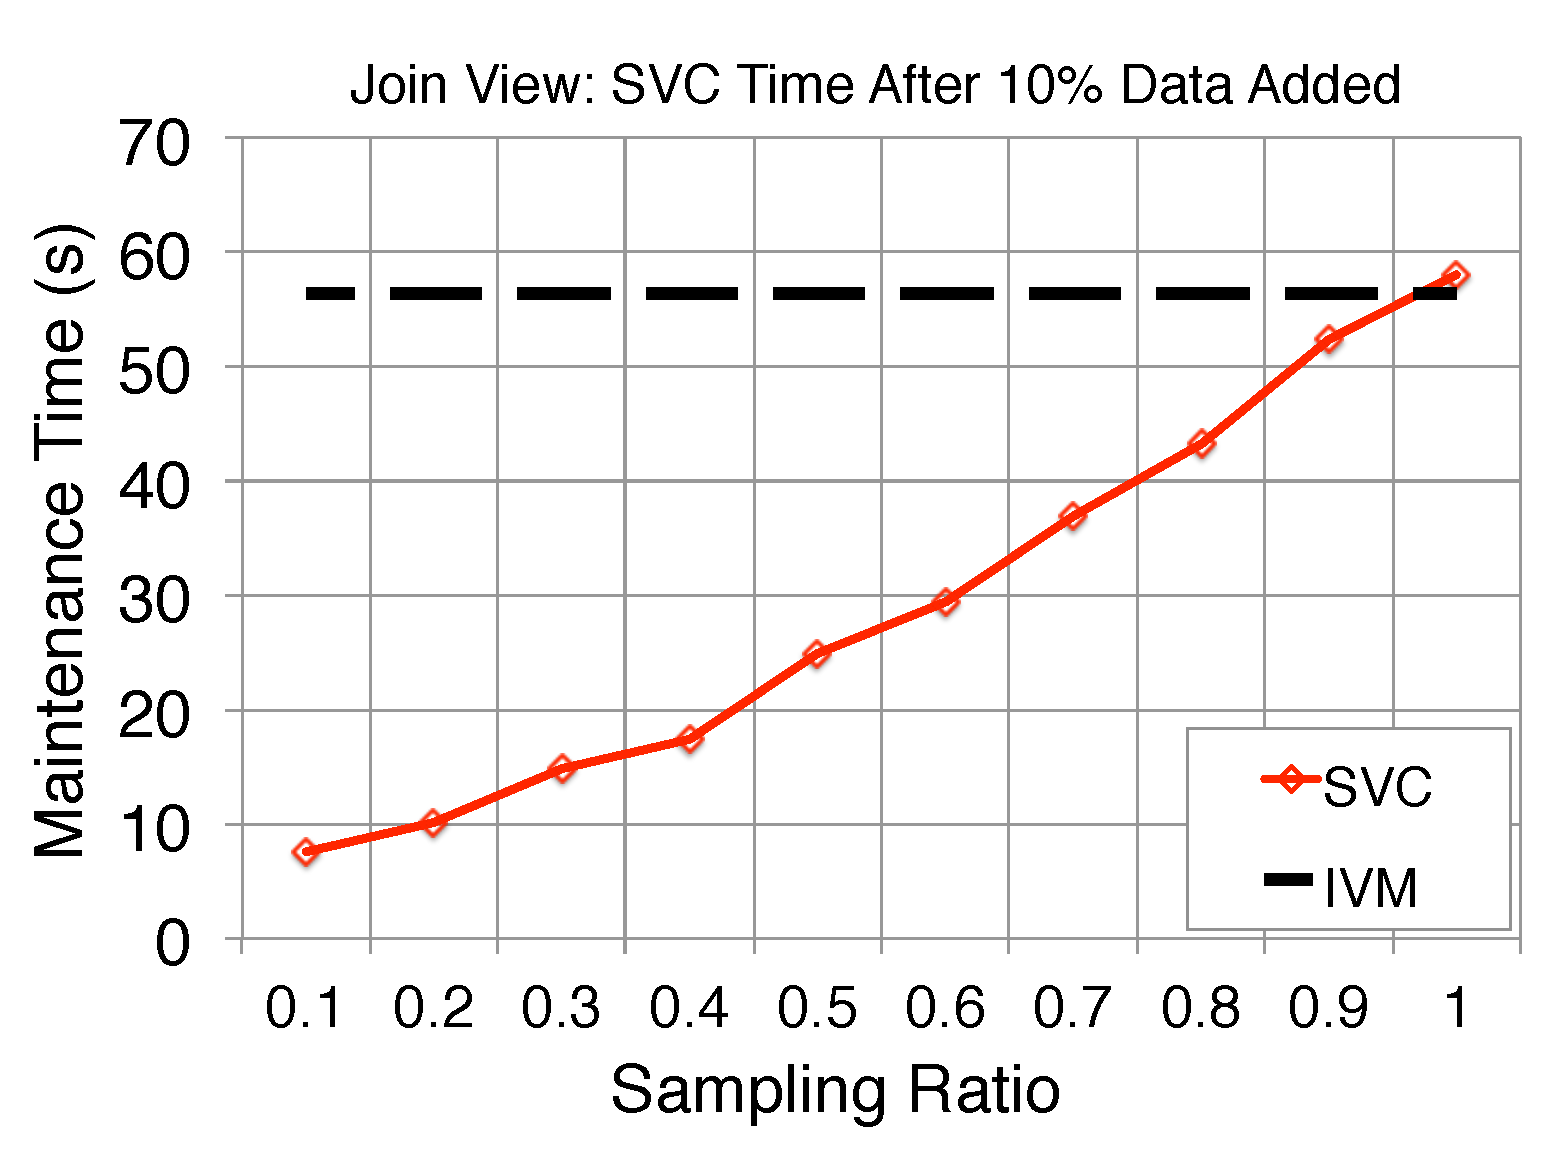
\includegraphics[scale=0.13]{exp/msj_1.pdf}
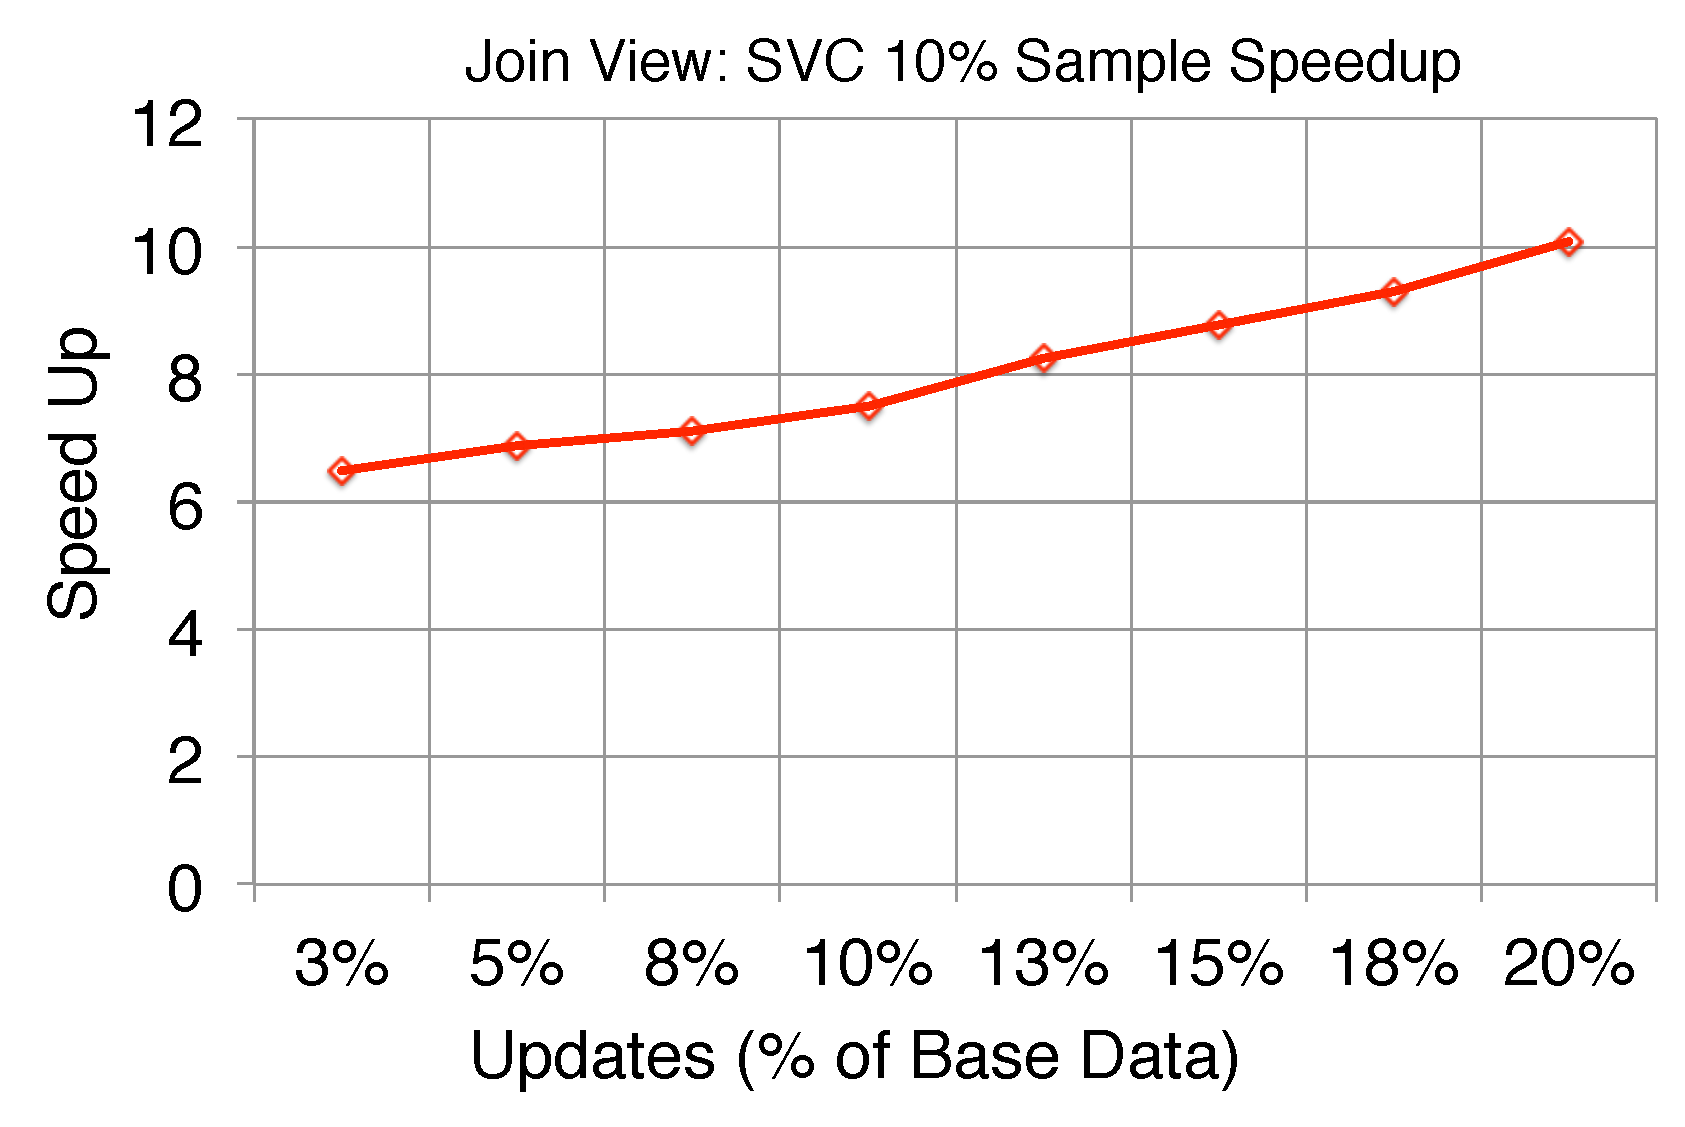
\includegraphics[scale=0.13]{exp/msj_2.pdf}\vspace{-1em}
 \caption{(a) On a 10GB dataset with 1GB of insertions and updates, we vary the sampling ratio and measure the maintenance time of \svc. The black line marks the time for full incremental view maintenance. (b) For a fixed sampling ratio of 10\%, we vary the update size and plot the speedup compared to full incremental maintenance for \svc. \vspace{-1em}\label{exp-1-samplesize}}
\end{figure}

\subsubsection{Metrics and Evaluation}
To illustrate how \svc gives the user access to this new trade-off space, we will illustrate that \svc is more accurate than the stale query result (No Maintenance); but is less computationally intensive than full IVM. 
In our evaluation, we separate maintenance from query processing.
We use the following notation to represent the different approaches:
\vspace{-.25em}
\begin{itemize}[noitemsep]
\item No maintenance (Stale): The baseline for evaluation is not applying any maintenance to the materialized view.
\item Incremental View Maintenance (IVM): We apply incremental view maintenance to the full view.
\item \svcnospace+AQP: We maintain a sample of the materialized view using \svc but estimate the result with AQP rather than using 
the correction technique proposed in this paper.
\item \svcnospace+Corr: We maintain a sample of the materialized view using \svc and process queries on the view using the correction method presented in this paper.
\end{itemize}
\vspace{-.25em}
%\reminder{Do you think we need to say something about another solution which maintains a sample of ``base'' table and transform a query on a view to a query on the base table?}
Since \svc has a sampling parameter, we denote a sample size of $x \% $ as \svcnospace+Corr-x or \svcnospace+AQP-x, respectively. 
To evaluate accuracy and performance, we define the following metrics:
\begin{itemize}[noitemsep]
\item Relative Error: For a query result $r$ and an incorrect result $r'$, the relative error is $\frac{\mid r-r' \mid}{r}.$
When a query has multiple results (a group-by query), then, unless otherwise noted, relative error is defined as the median over all the errors.
\item Maintenance Time: We define the maintenance time as the time needed to produce the up-to-date view for incremental view maintenance, and the time needed to produce the up-to-date sample in \svc. 
\end{itemize}

\subsection{Single-node Accuracy and Performance}
\vspace{-.5em}
\subsubsection{Join View}



\begin{figure}[t]
\centering
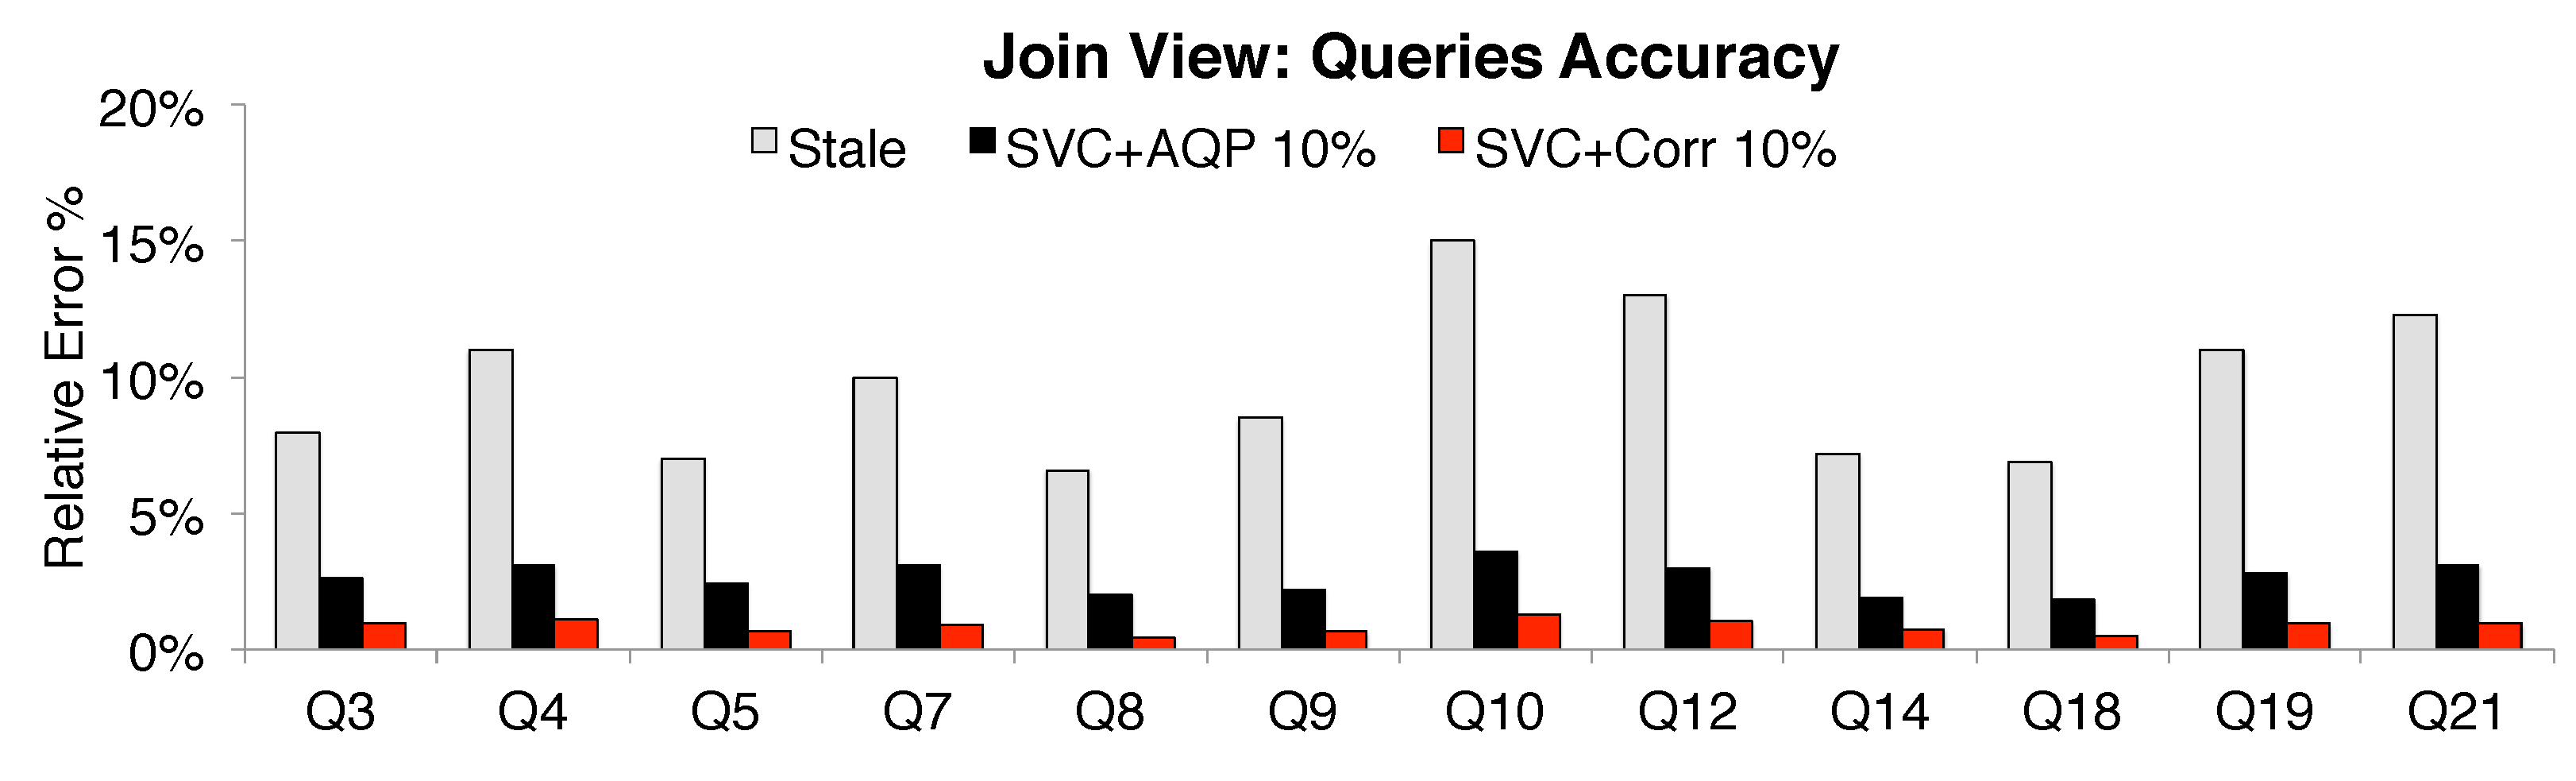
\includegraphics[scale=0.13]{exp/msj_3.pdf}\vspace{-.5em}
 \caption{We generate 100 of each TPCD parameterized query and answer it using the stale materialized view, \svcnospace+Corr, and \svcnospace+AQP. We plot the median relative error for each query (since the result for each query might be multi-valued).\label{exp-1-acc}}
\end{figure}

\begin{figure}[t]\vspace{-2em}
\centering
 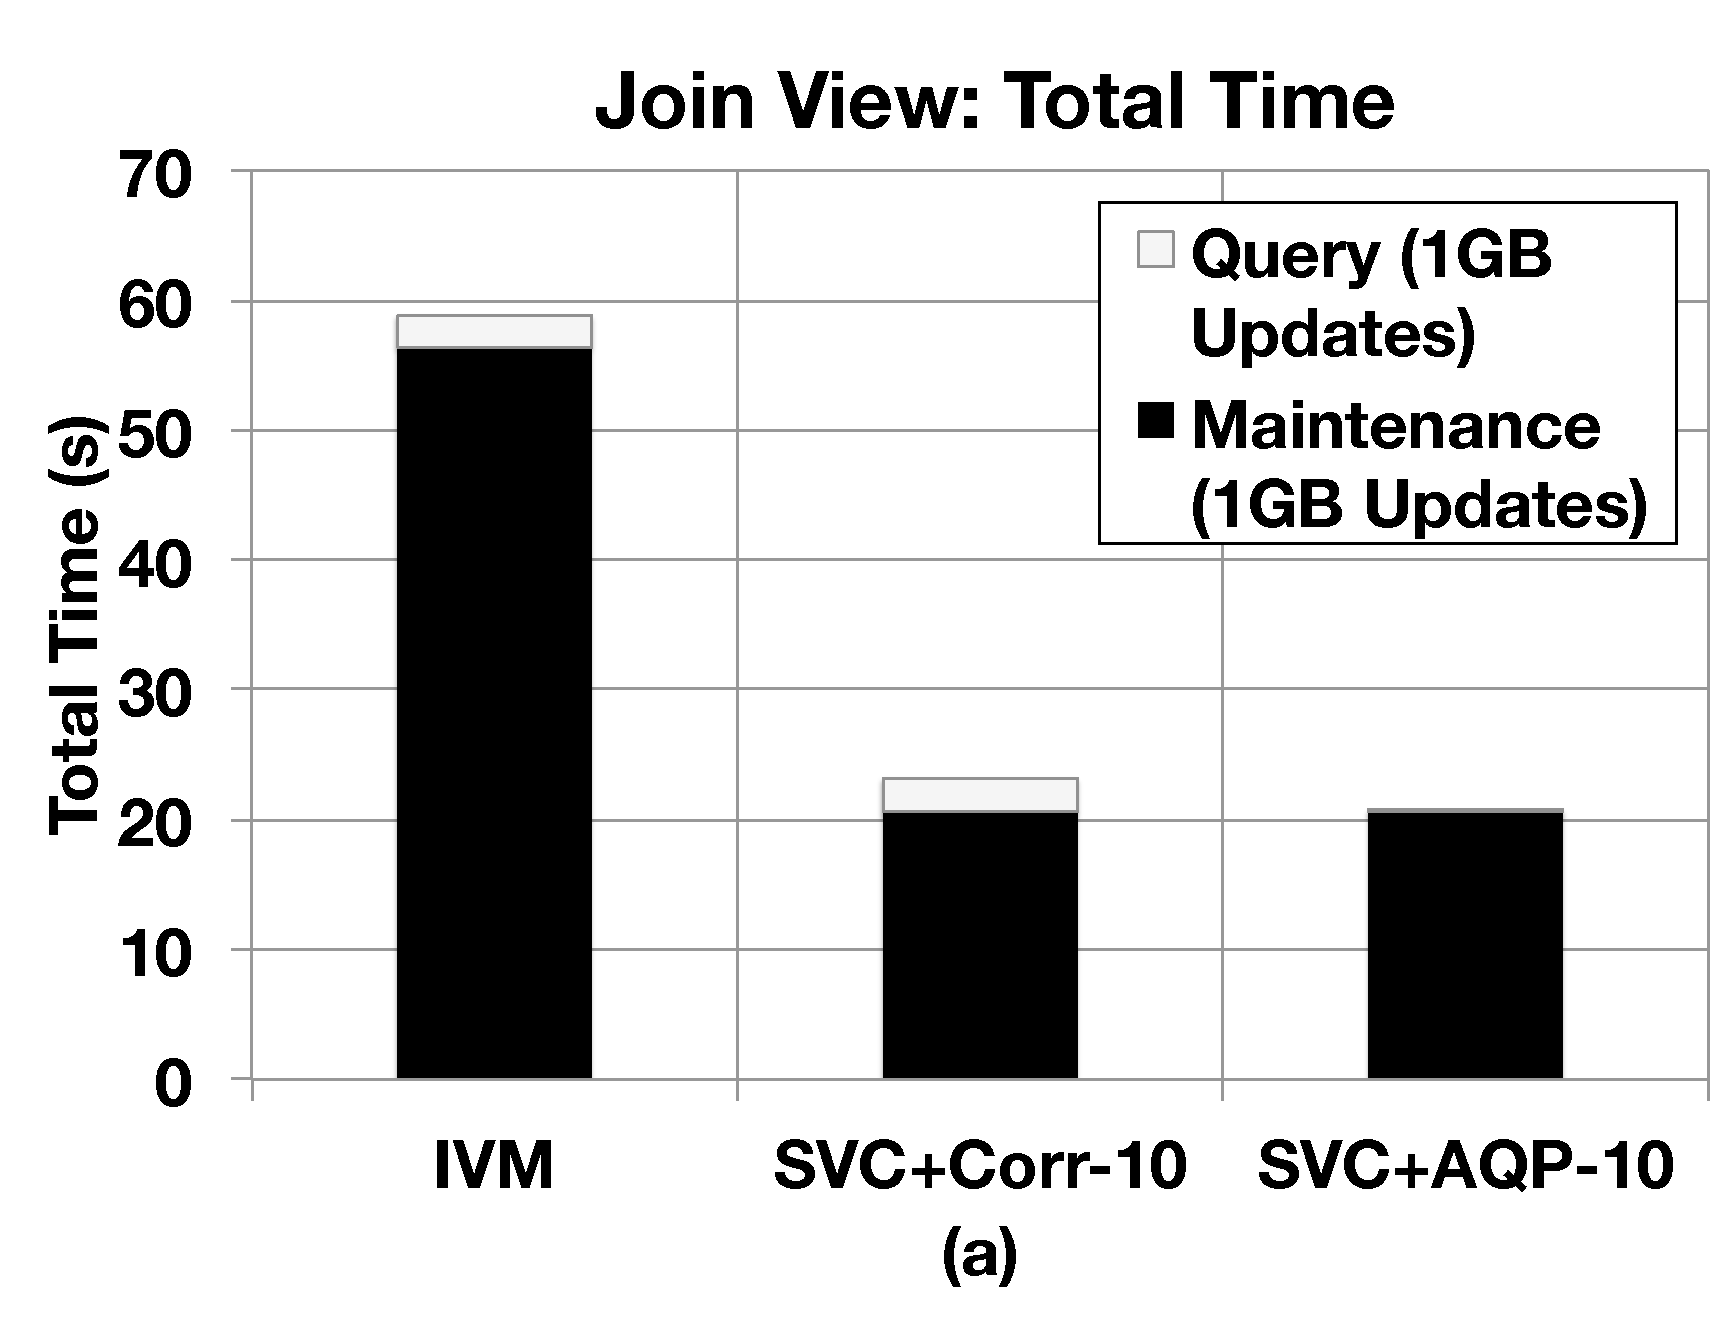
\includegraphics[scale=0.13]{exp/msj_4.pdf}
 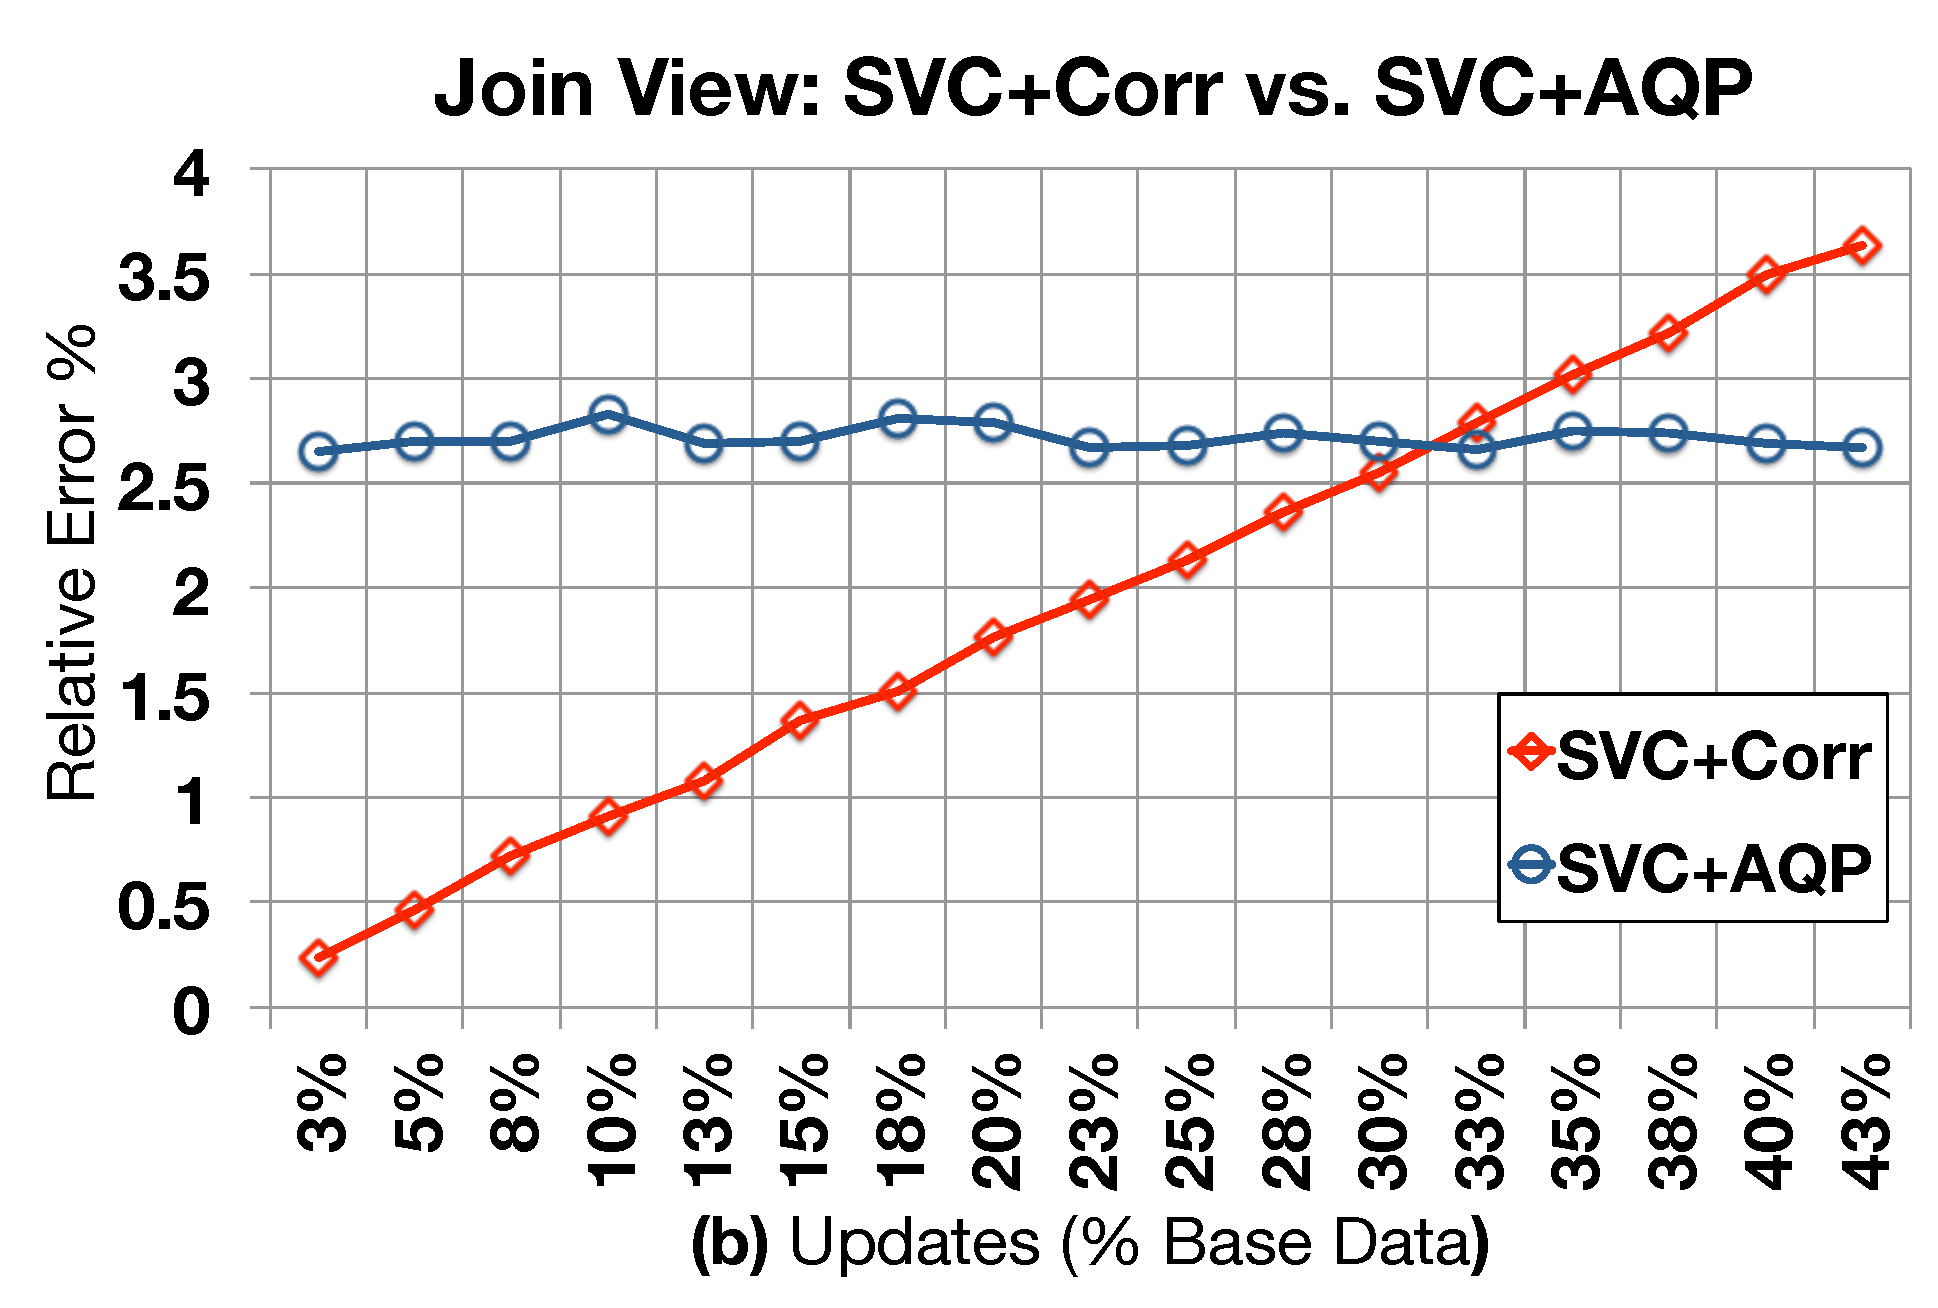
\includegraphics[scale=0.13]{exp/msj_6.pdf}\vspace{-.5em}
  \caption{(a) For a fixed sampling ratio of 10\% and update size of 10\% (1GB), we measure the total time incremental maintenance + query time. \svcnospace+Corr does take longer to query a view (due to the correction) than \svcnospace+AQP and IVM, but this overhead is small relative to to the savings in maintenance time. (b) We vary the update rate to show that \svcnospace+Corr is more accurate than \svcnospace+AQP until the update size is 32.5\% (3.2GB). \vspace{-1.5em} \label{exp-1-total}}
\end{figure}

%\begin{figure}[t]
%\centering
%  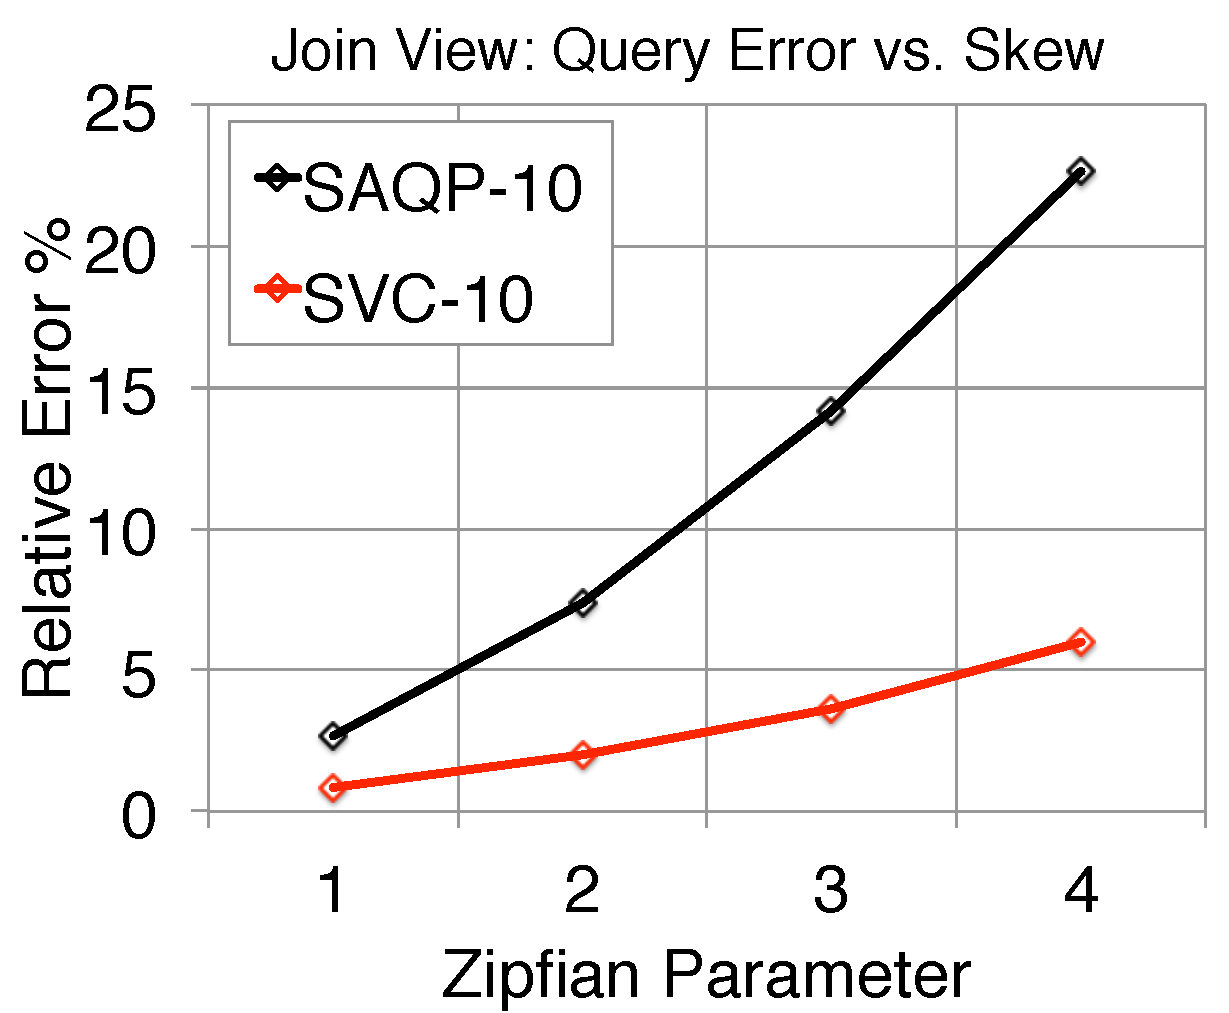
\includegraphics[scale=0.16]{exp/msj_5.pdf}
% \caption{We fix the update size at 1GB and the sampling ratio at 10\% and vary the skew of the dataset. The gap between \svcnospace+AQP and \svc increases in more skew datasets suggesting that corrections are more robust to skew. \label{exp-1-zipf}}
%\end{figure}

In our first experiment, we evaluate how \svc performs on a materialized view of the join of \textsf{lineitem} and \textsf{orders}.
We generate a 10GB base TPCD dataset with skew $z=1$, and derive the view from this dataset.
We first generate 1GB (10\% of the base data) of updates (insertions and updates to existing records), and vary the sample size.

\textbf{Performance: }
Figure \ref{exp-1-samplesize}(a), shows the maintenance time of \svc as a function of sample size.
With the bolded dashed line, we note the time for full IVM. 
For this materialized view, sampling allows for significant savings in maintenance time; albeit for approximate answers.
While full incremental maintenance takes 56 seconds, \svc with a 10\% sample can complete in 7.5 seconds.

The speedup for \svc-10 is 7.5x which is far from ideal on a 10\% sample.
In the next figure, Figure \ref{exp-1-samplesize}(b), we evaluate this speedup. 
We fix the sample size to 10\% and plot the speedup of \svc compared to IVM while varying the size of the updates.
On the x-axis is the update size as a percentage of the base data.
For small update sizes, the speedup is smaller, 6.5x for a 2.5\% (250GB) update size.
As the update size gets larger, \svc becomes more efficient, since for a 20\% update size (2GB), the speedup is 10.1x. 
The super-linearity is because this view is a join of \textsf{lineitem} and \textsf{orders} and we assume that there is not a join index on the updates.
Since both tables are growing sampling reduces computation super-linearly. 

\textbf{Accuracy: }
At the same design point with a 10\% sample, we evaluate the accuracy of \svc.
In Figure \ref{exp-1-acc}, we answer TPCD queries with this view.
The TPCD queries are group-by aggregates and we plot the median relative error for \svcnospace+Corr, No Maintenance, and \svcnospace+AQP.
On average over all the queries, we found that \svcnospace+Corr was 11.7x more accurate than the stale baseline, and 3.1x more accurate than applying \svcnospace+AQP to the sample.

\textbf{\svcnospace+Corr vs. \svcnospace+AQP: }
While more accurate, it is true that \svcnospace+Corr correction technique moves some of the computation from maintenance to query execution.
\svcnospace+Corr calculates a correction to a query on the full materialized view.
On top of the query time on the full view (as in IVM) there is additional time to calculate a correction from a sample.
On the other hand \svcnospace+AQP runs a query only on the sample of the view, 
We evaluate this overhead in Figure \ref{exp-1-total}(a), where we compare the total time maintenance and query execution time.
For a 10\% sample \svcnospace+Corr required 2.69 secs to execute a \sumfunc over the whole view, IVM required 2.45 secs, and  \svcnospace+AQP required 0.25 secs.
However, when we compare this overhead to the savings in maintenance time it is small.


\svcnospace+Corr is most accurate when the materialized view is less stale, since it relies on correct a stale result.
On the other hand \svcnospace+AQP is more robust to the staleness and gives a consistent relative error.
The error for \svcnospace+Corr grows proportional to the staleness.
In Figure \ref{exp-1-total}(b), we explore which query processing technique should be used \svcnospace+Corr or \svcnospace+AQP.
For a 10\% sample, we find that \svcnospace+Corr is more accurate until the update size is 32.5\% of the base data.

%\textbf{Effect of Skew: }
%Finally in Figure \ref{exp-1-zipf}, we vary the Zipfian parameter and show how the accuracy of \svcnospace+Corr and \svcnospace+AQP changes.
%While both techniques are sensitive to skew, we find that the gap between \svcnospace+Corr and \svcnospace+AQP widens for more skewed datasets. 
%\svc's accuracy is dependent on the variance of the difference between tuples in the up-to-date view and the stale view; which is different from \svcnospace+AQP which is dependent on the variance of the tuples themselves. 
%Even though a dataset might be skewed, if (in relative terms) the updates are more uniform \svcnospace+Corr will give more accurate results.
%We can make \svcnospace+Corr and \svcnospace+AQP even more accurate using the outlier indexing which we will evaluate in the later sections.



\subsubsection{Aggregate View}
\label{exp-datacube}

\begin{figure}[t]
\centering
 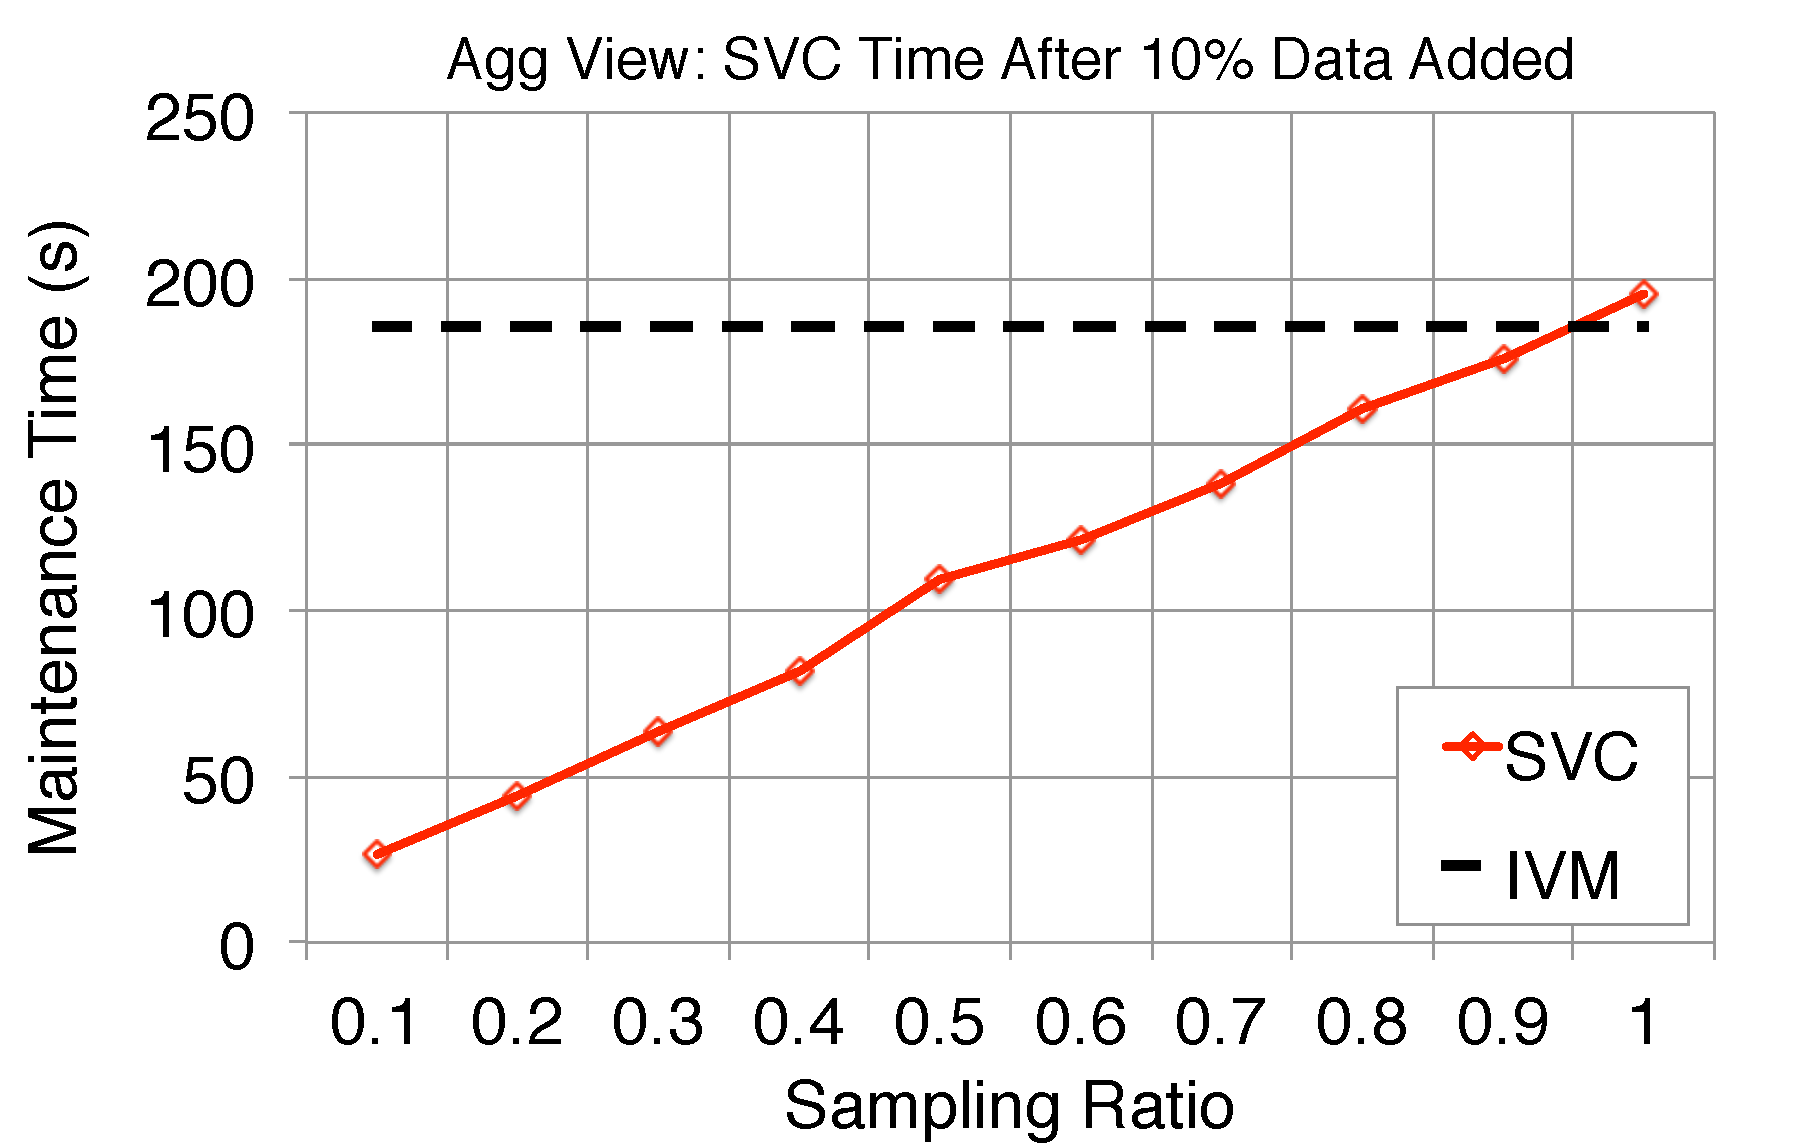
\includegraphics[scale=0.13]{exp/msdc_1.pdf}
 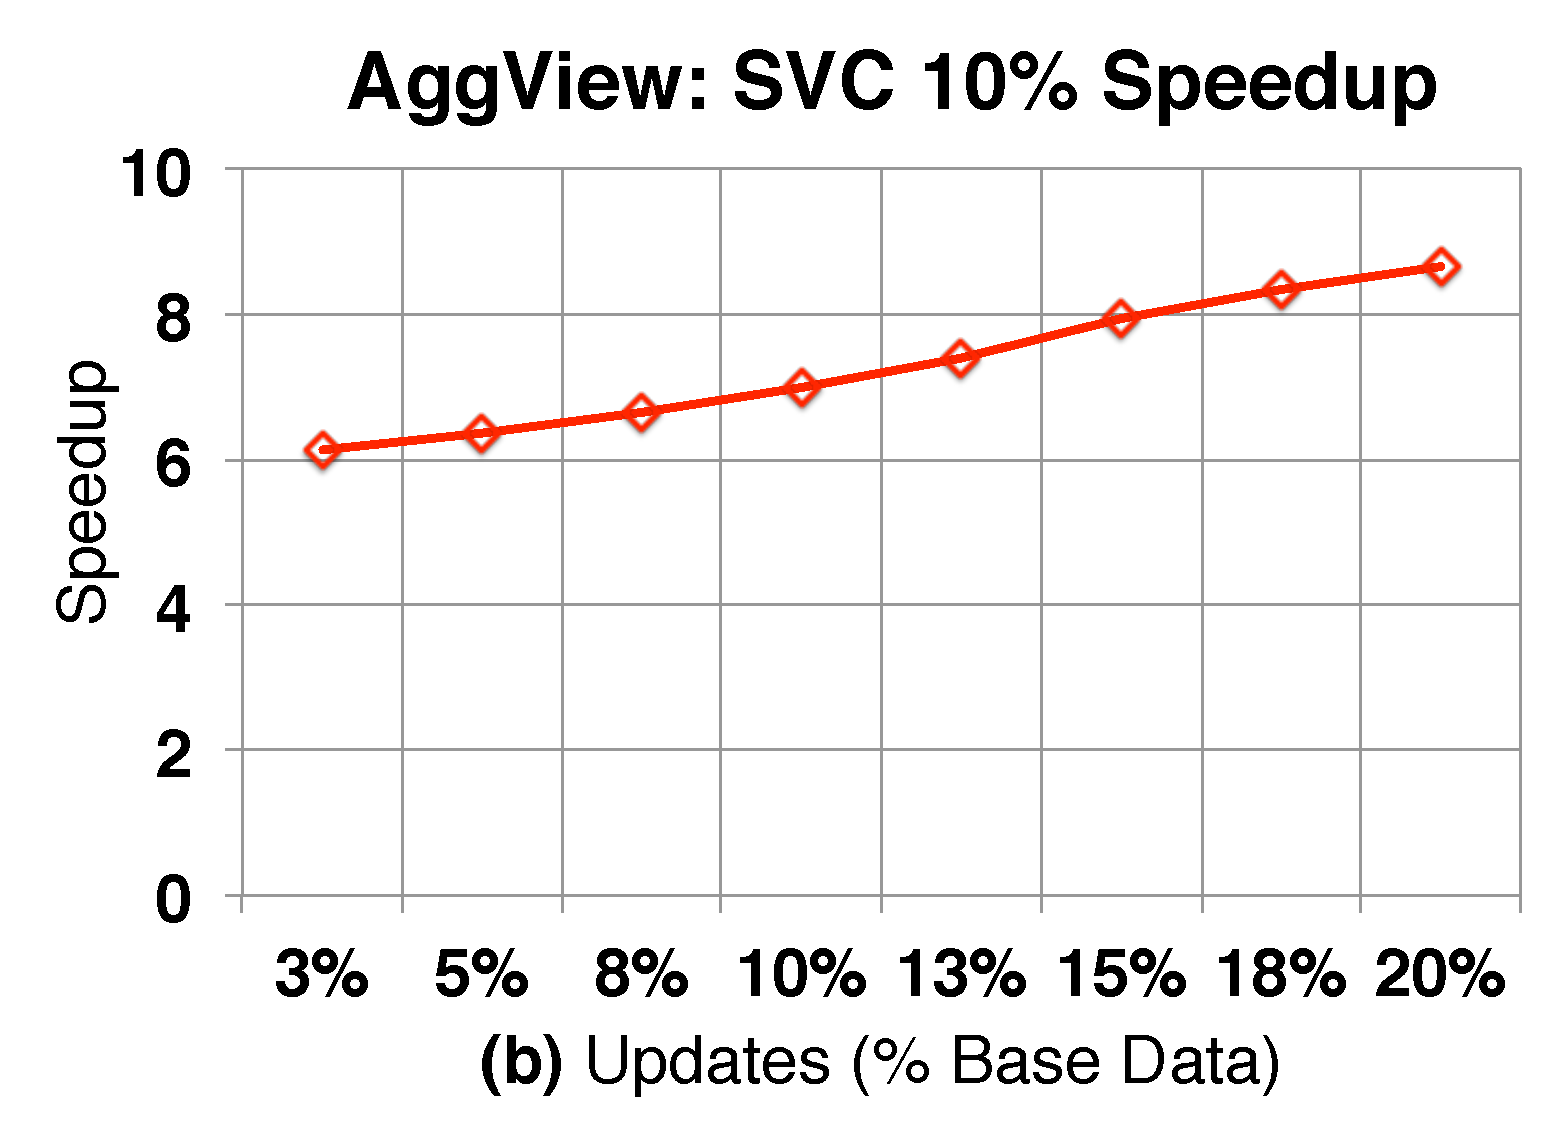
\includegraphics[scale=0.13]{exp/msdc_2.pdf}\vspace{-.5em}
  %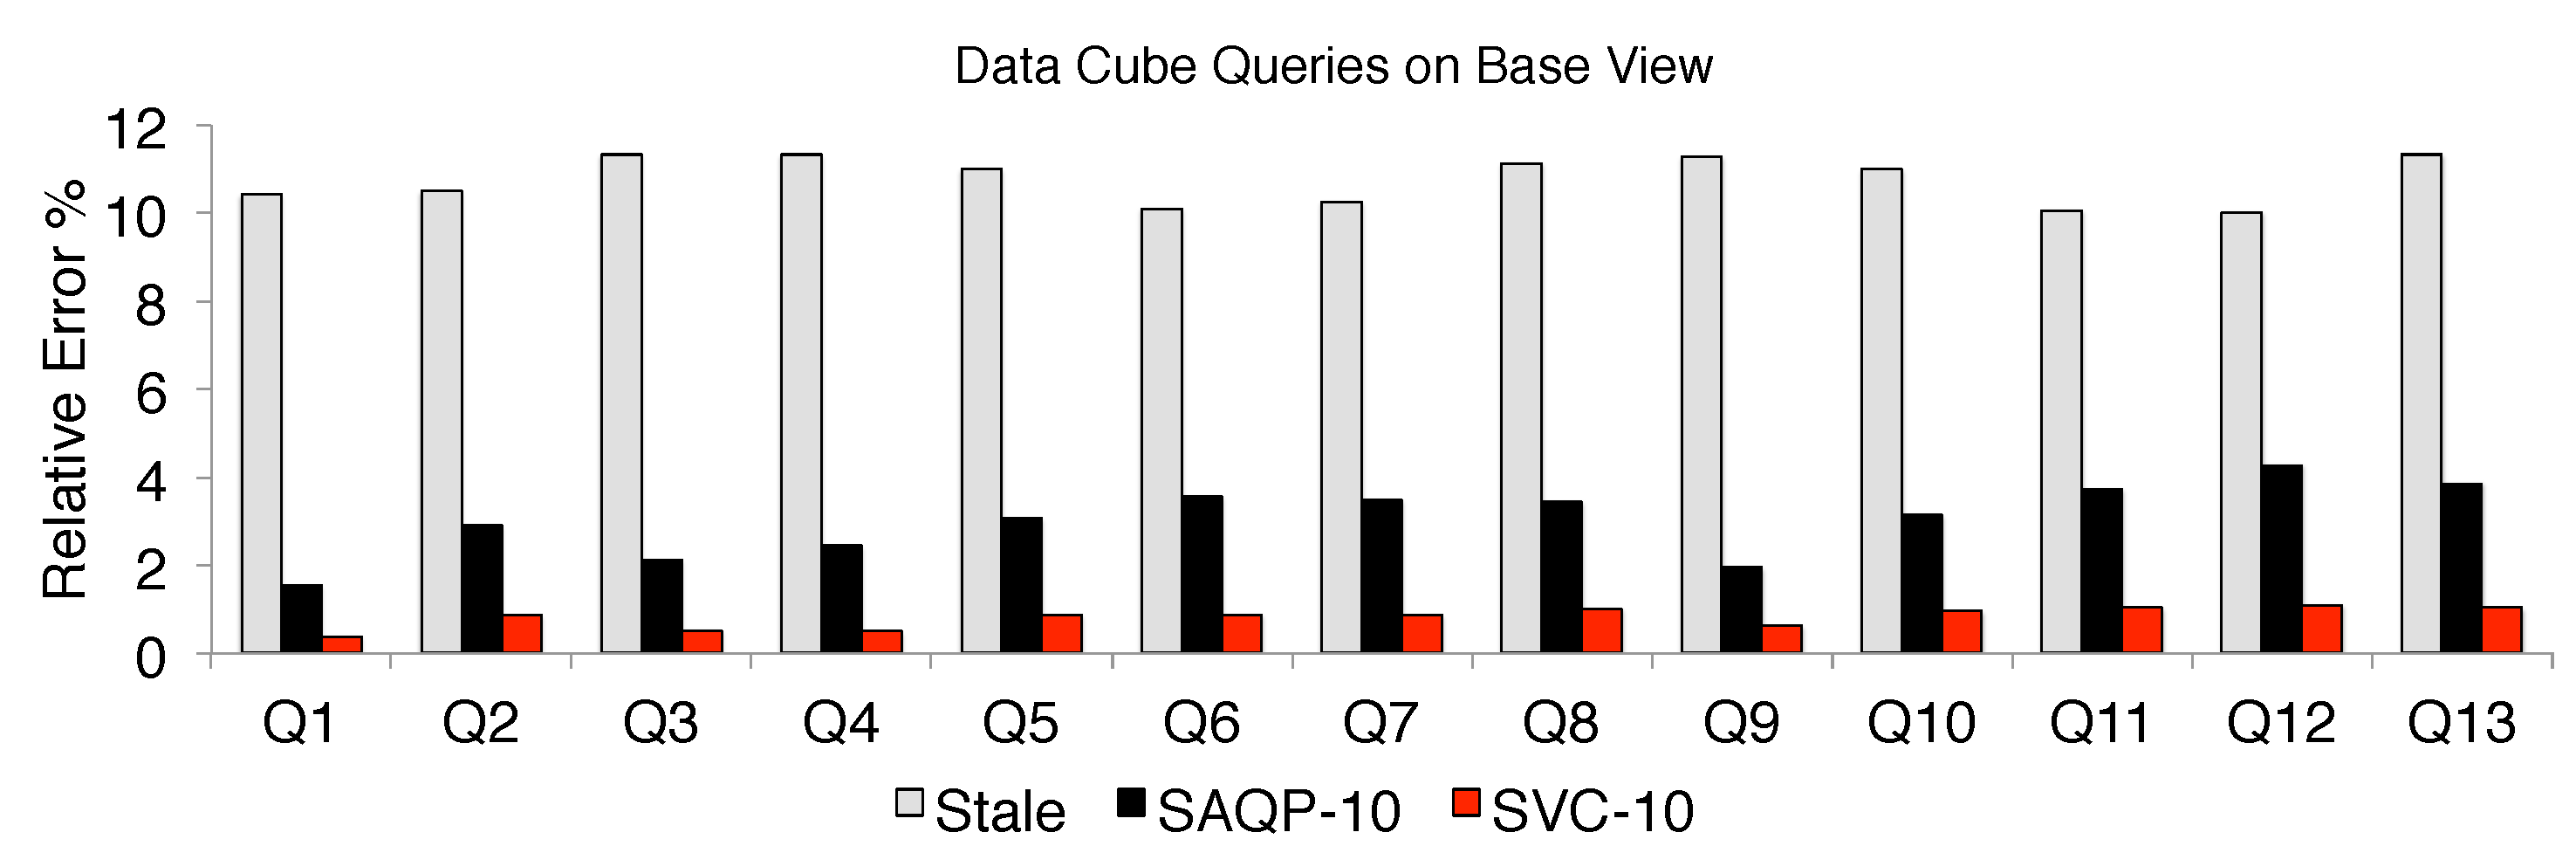
\includegraphics[scale=0.17]{exp/msdc_3.pdf}
   \caption{(a) On a 10GB dataset with 1GB of insertions and updates, we vary the sampling ratio and measure the maintenance time of \svc. The black line marks the time for full incremental view maintenance. (b) For a fixed sampling ratio of 10\%, we vary the update size and plot the speedup compared to full incremental maintenance for \svc.\label{exp2-acc-sample}}
\end{figure}


\begin{figure}[t]\vspace{-.5em}
\centering
 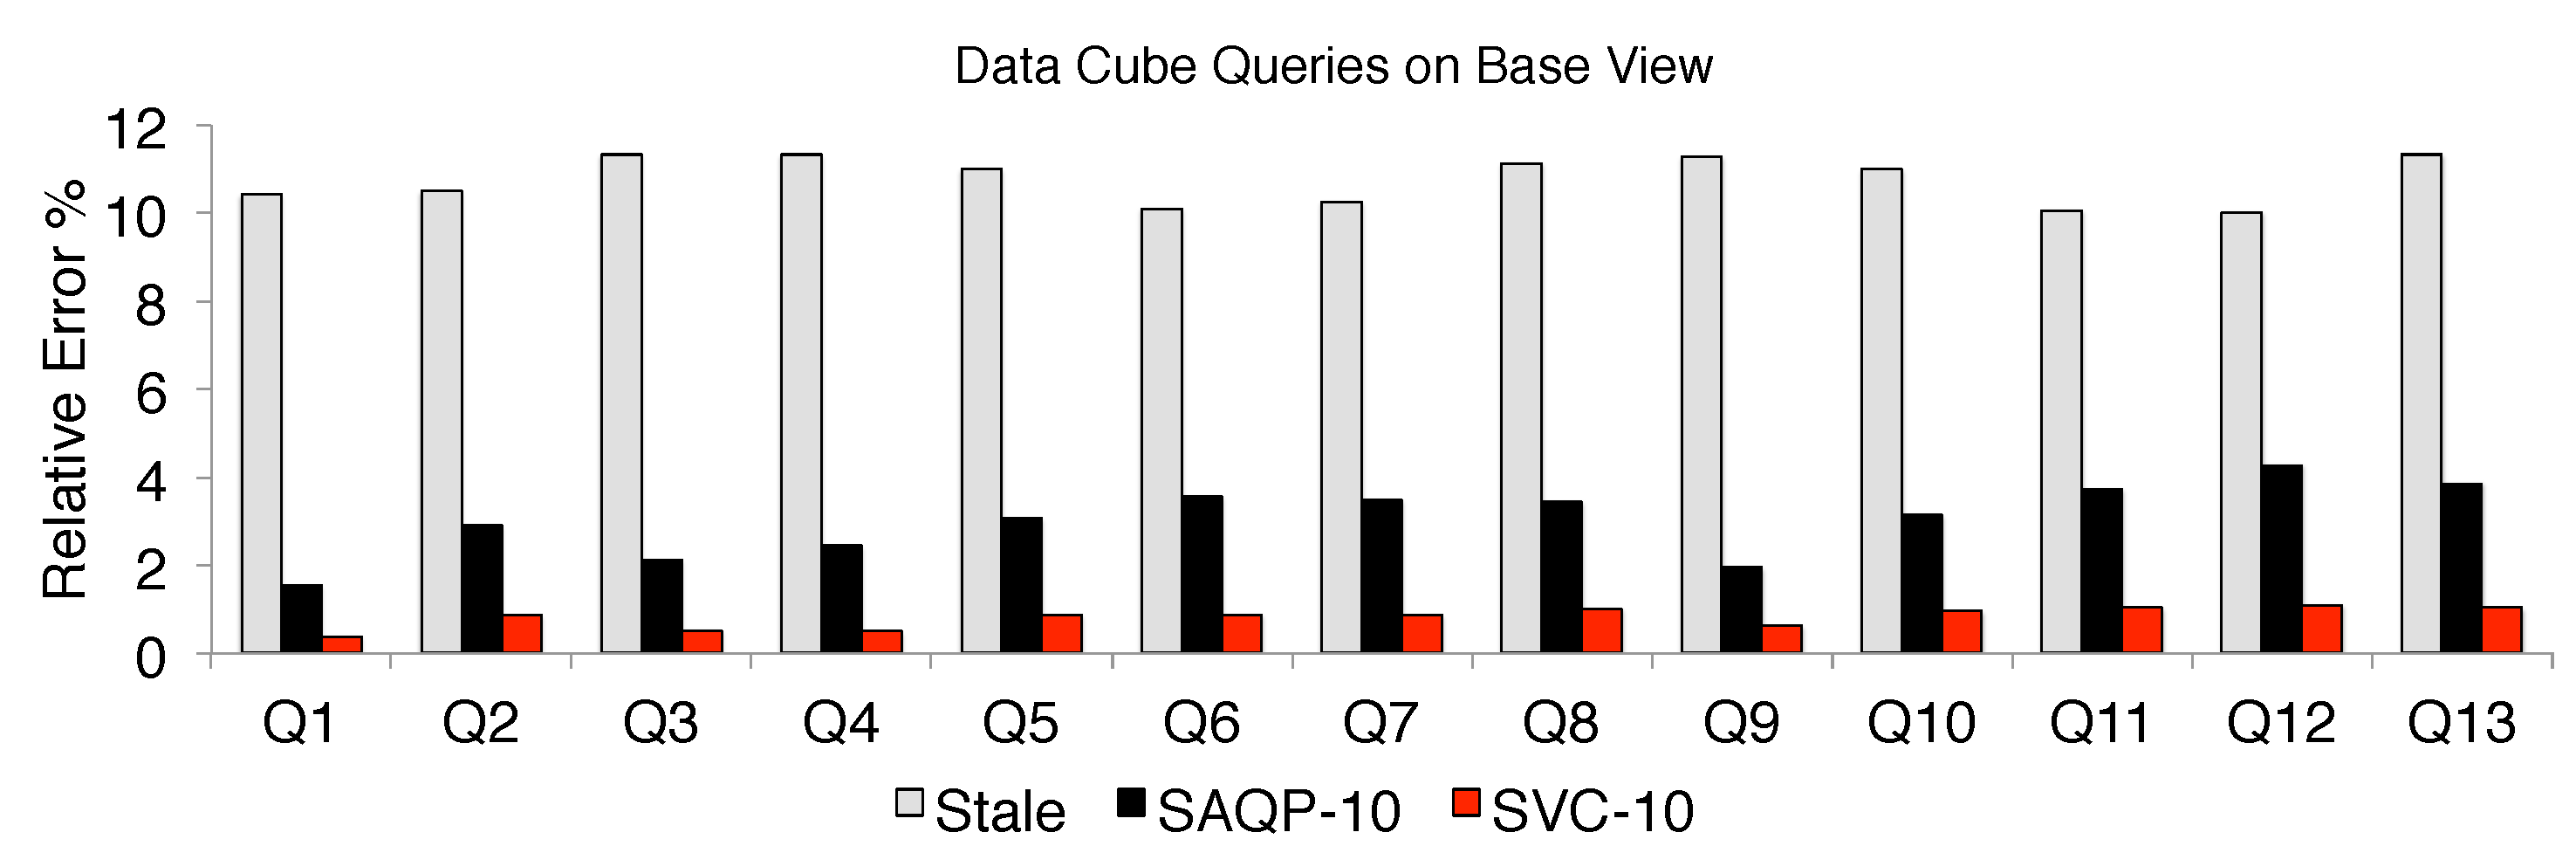
\includegraphics[scale=0.13]{exp/msdc_3.pdf}\vspace{-.5em}
 %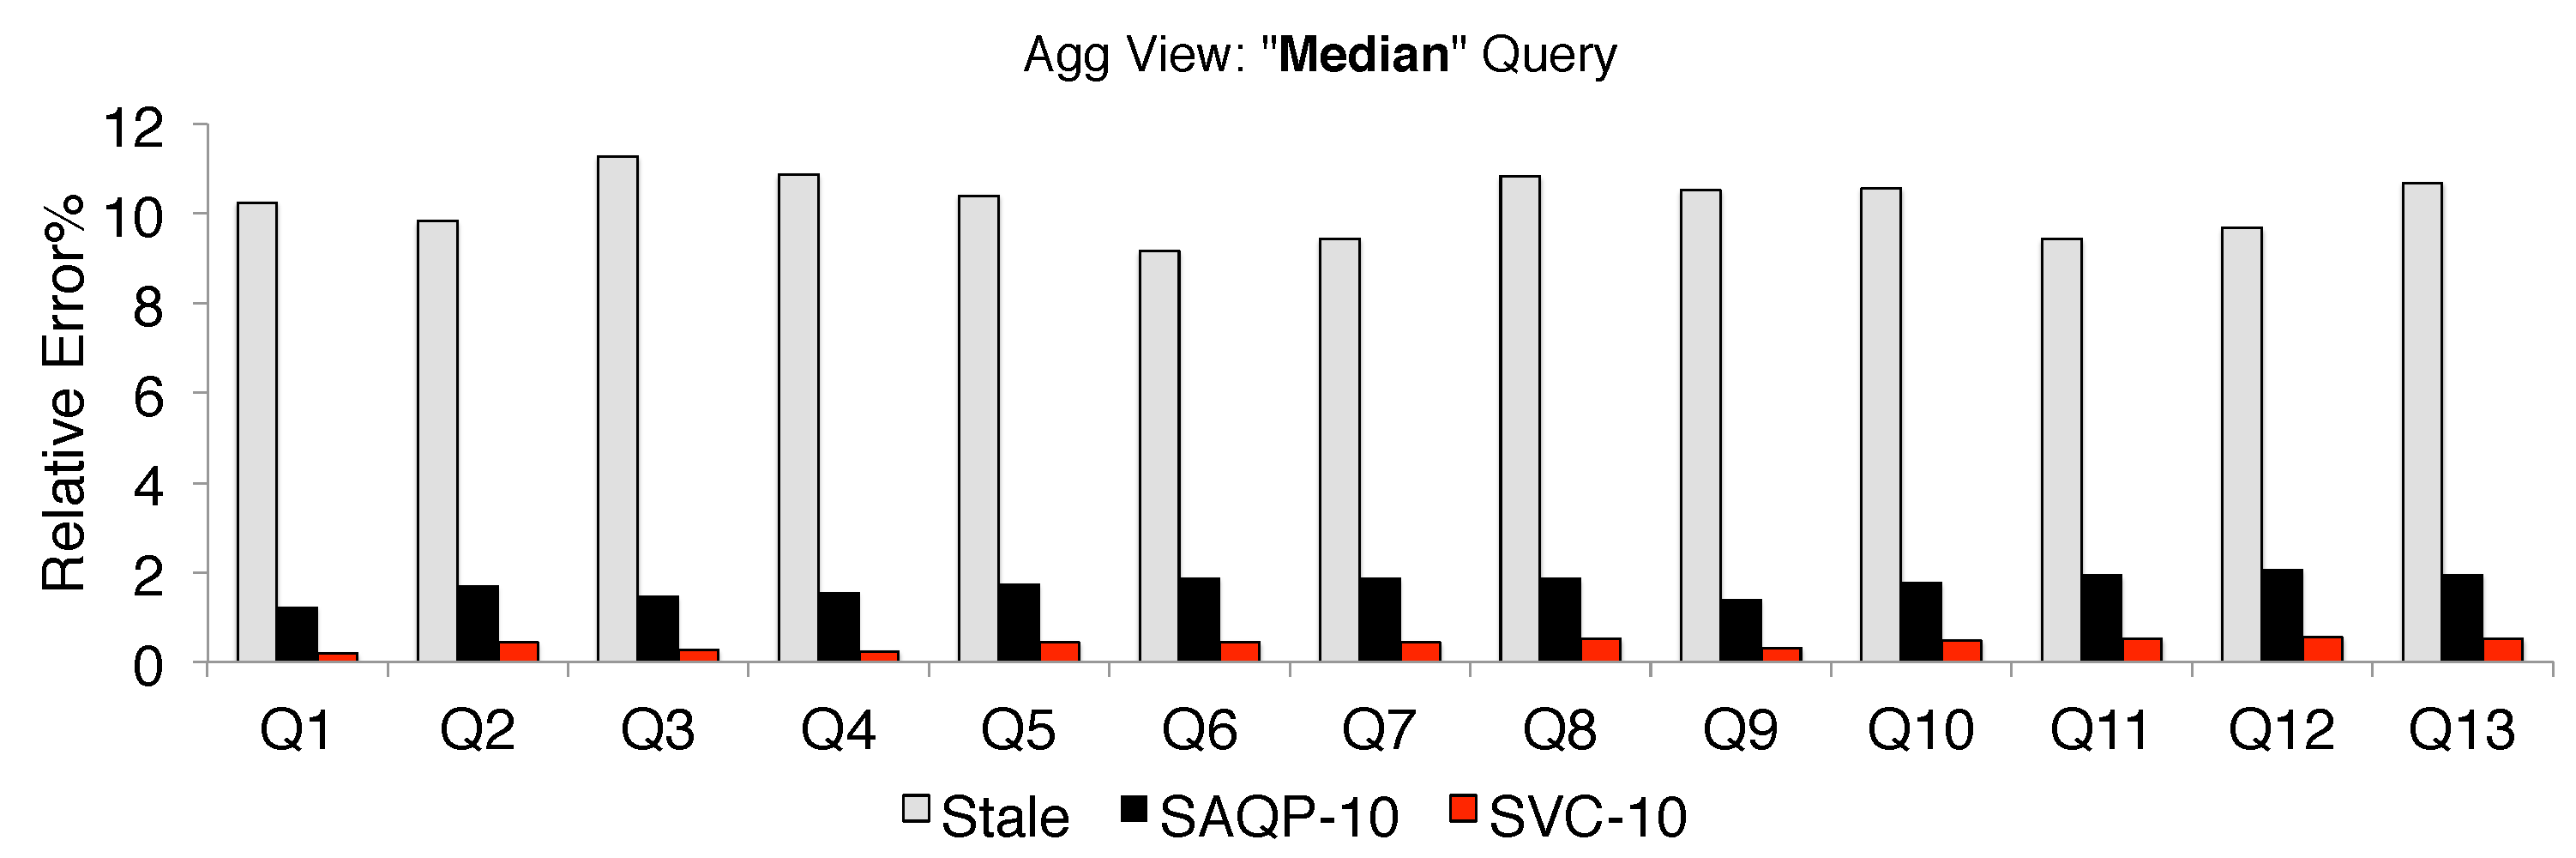
\includegraphics[scale=0.13]{exp/msdc_5.pdf}
   \caption{We measure the accuracy of each of the roll-up aggregate queries on this view. For a 10\% sample size and 10\% update size, we find that \svcnospace+Corr is more accurate than \svcnospace+AQP and No Maintenance.\vspace{-.5em}\label{exp2-acc-sample2}}
\end{figure}



%\begin{figure}[t]
%\centering
%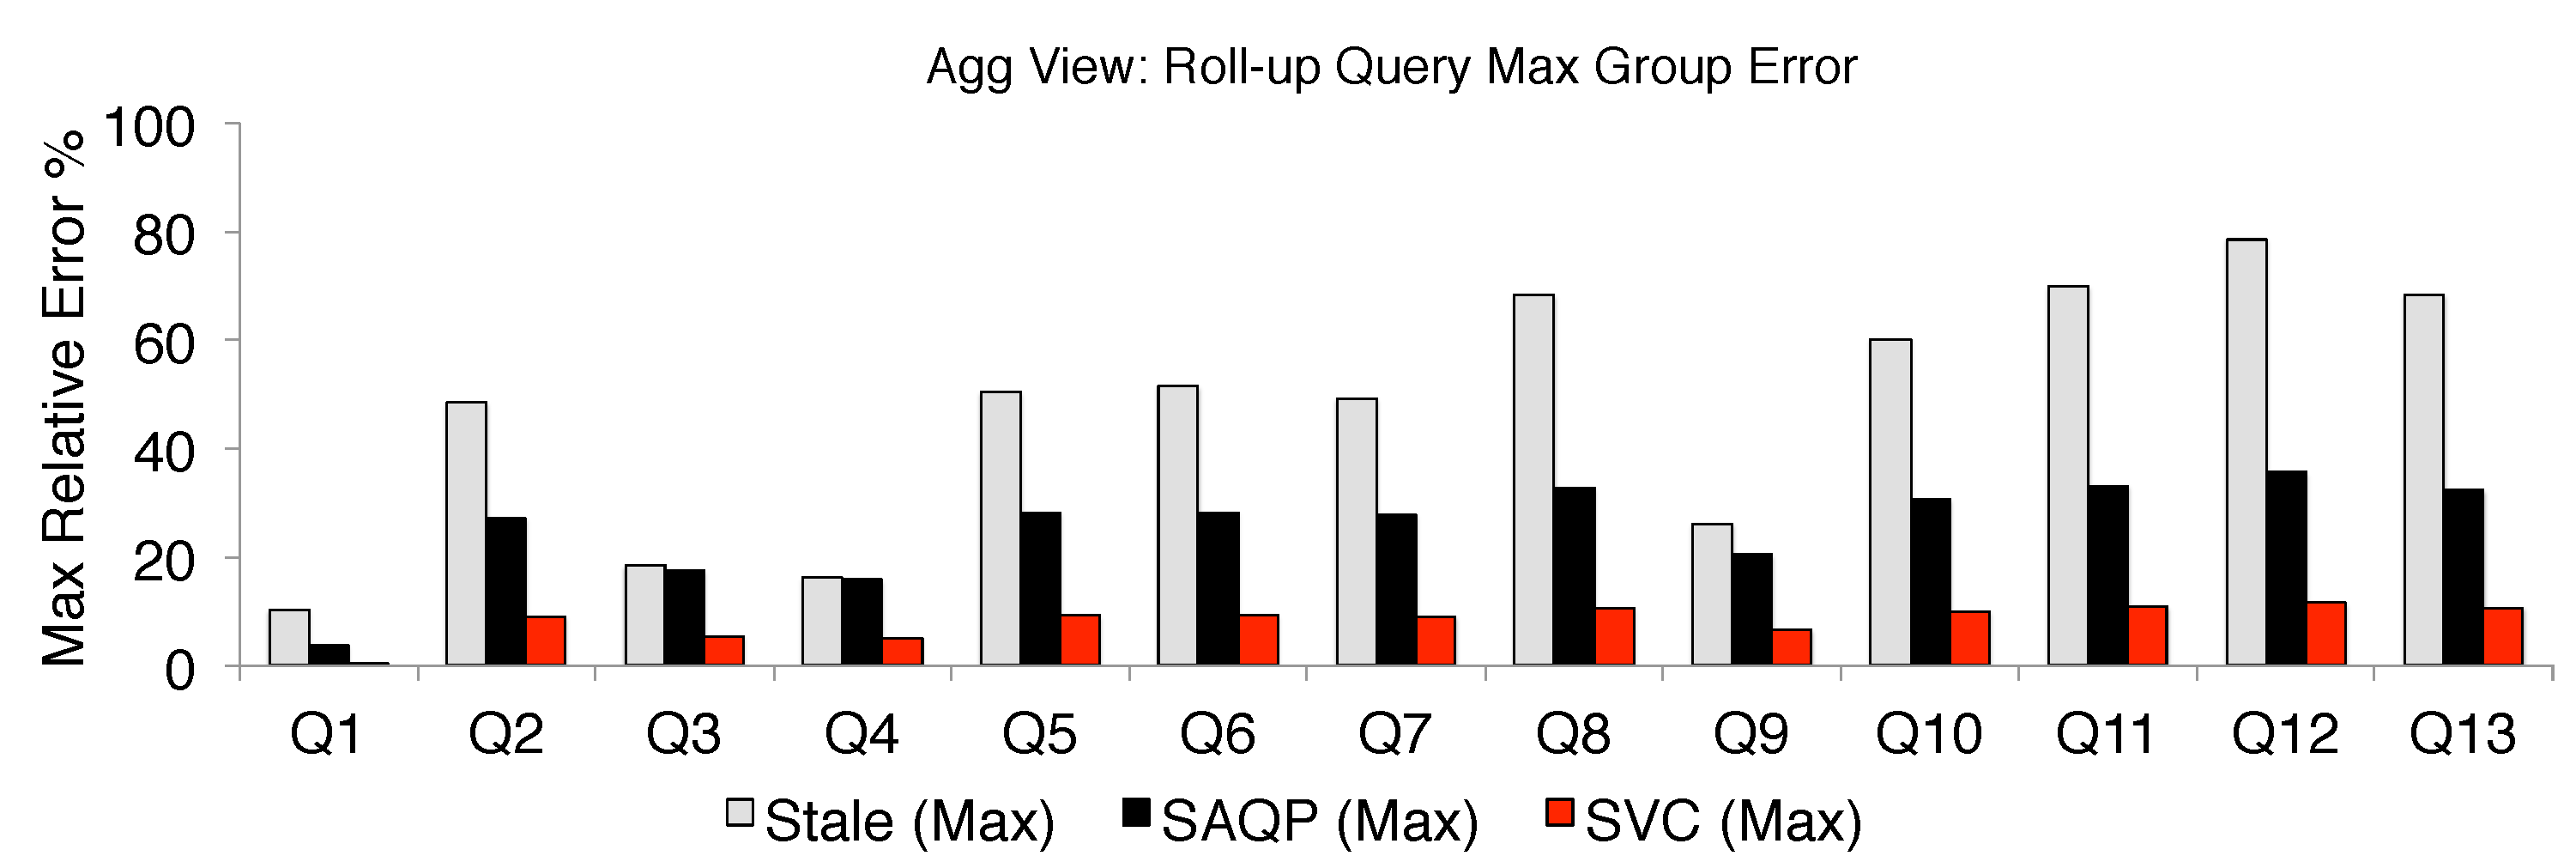
\includegraphics[scale=0.17]{exp/msdc_4.pdf}
%   \caption{For 1GB of updates, we plot the max error as opposed to the median error in the previous experiments. Even though updates are 10\% of the dataset size, some queries are nearly 80\% incorrect. \svc helps significantly mitigate this error. \label{exp2-max}}
%\end{figure}

%\begin{figure}[t]
%\centering
%  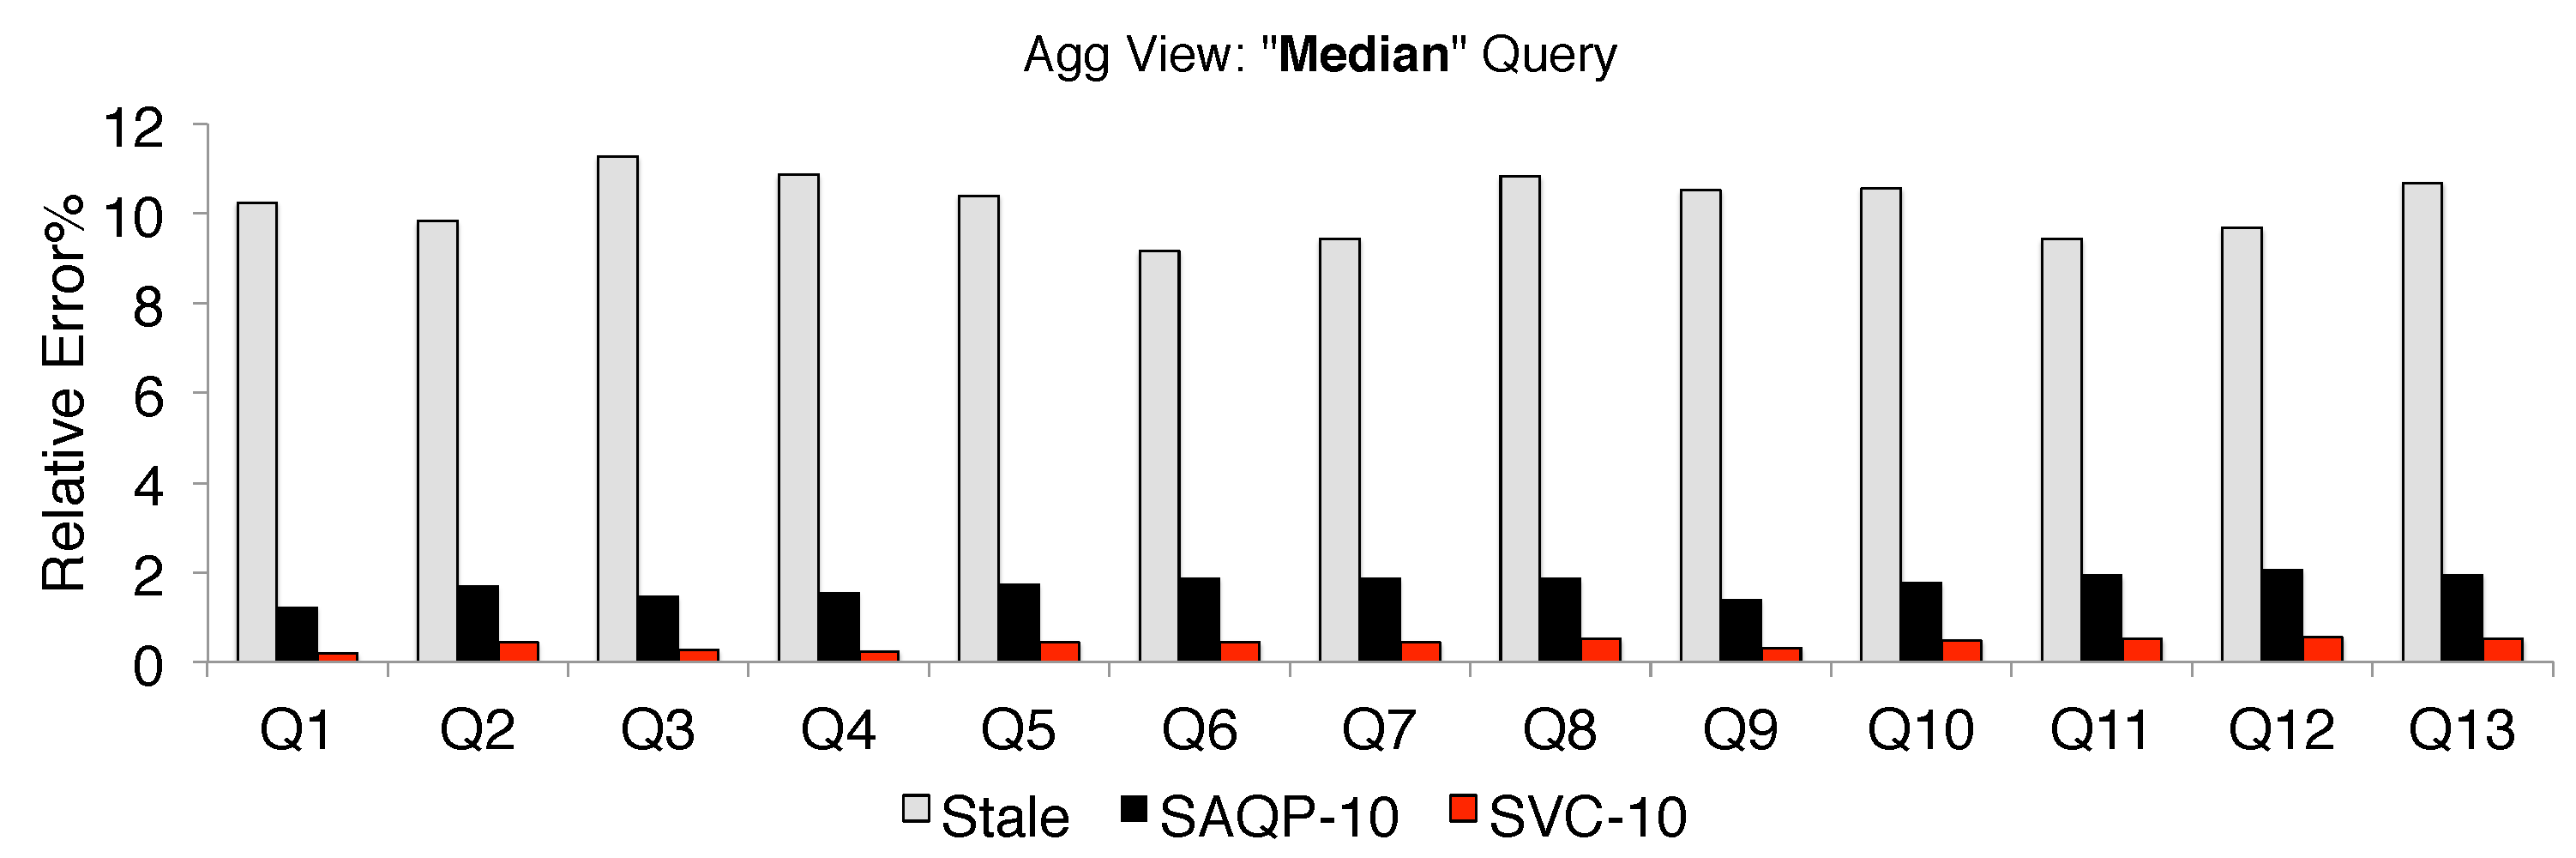
\includegraphics[scale=0.14]{exp/msdc_5.pdf}
  %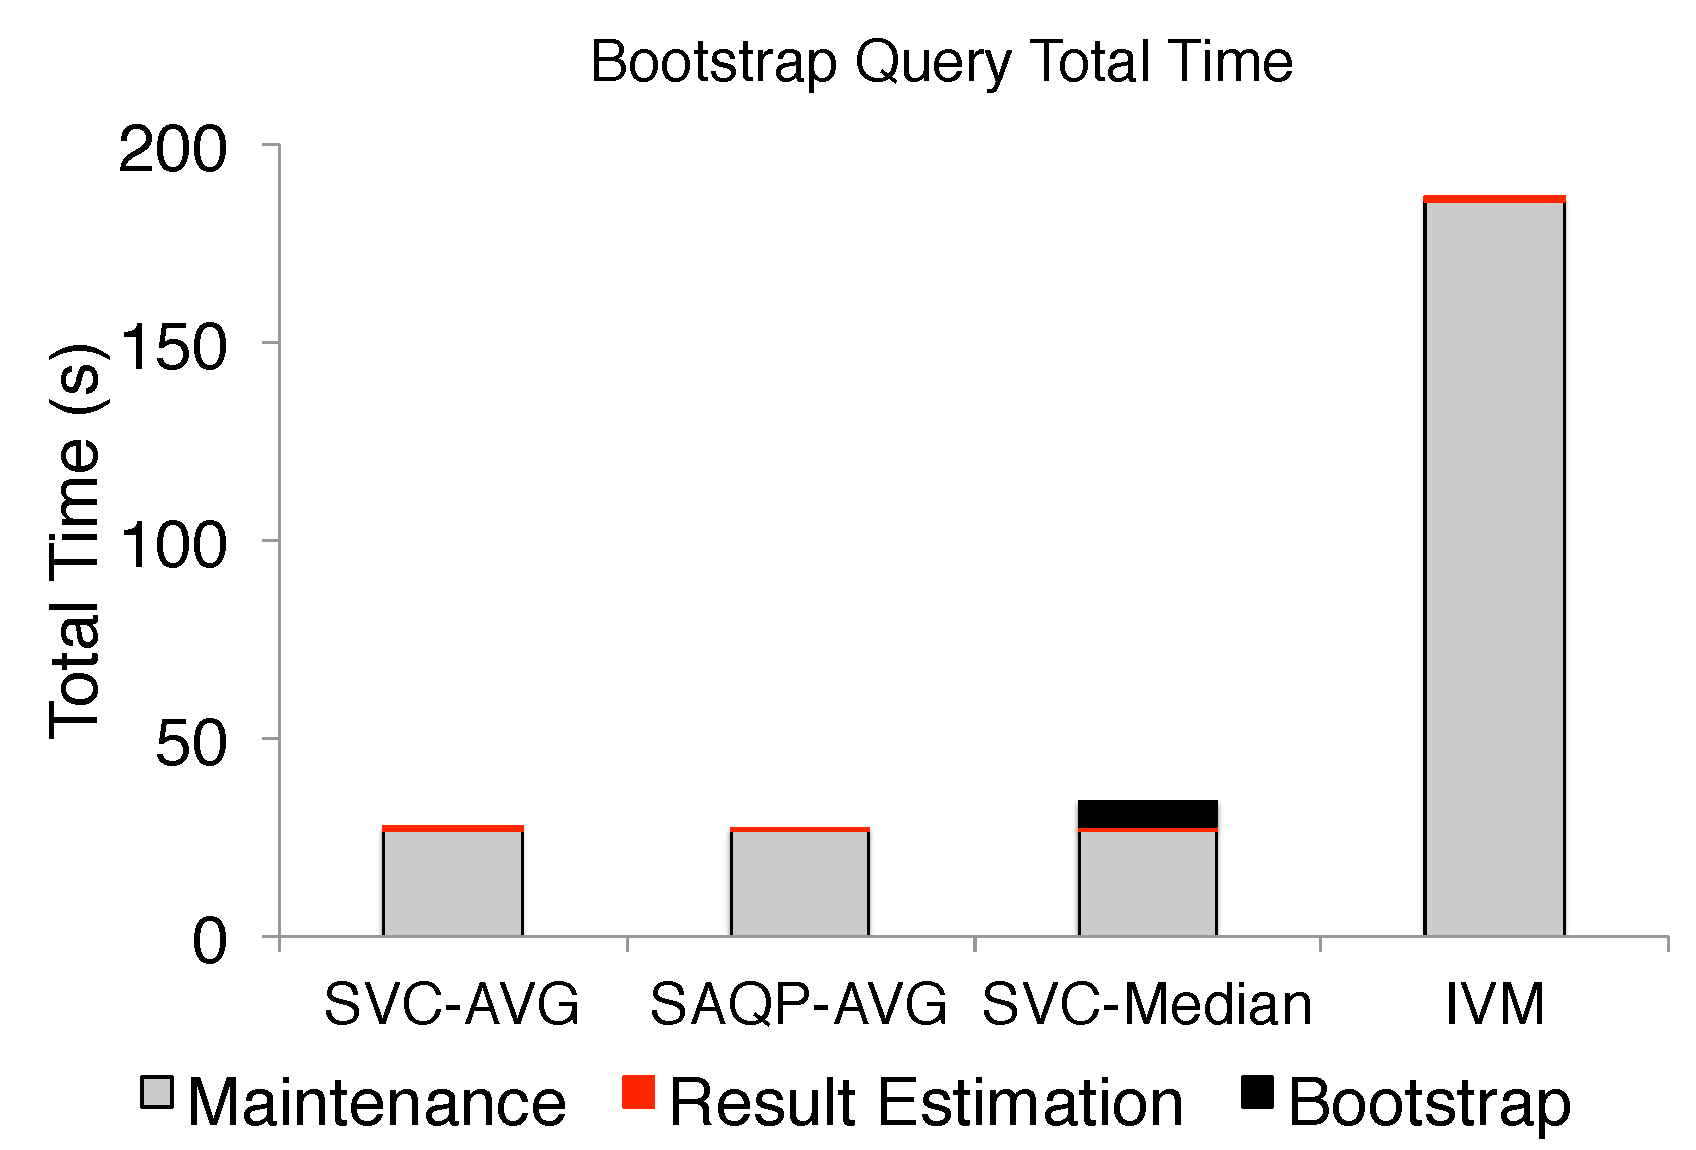
\includegraphics[scale=0.20]{exp/msdc_6.pdf}
% \caption{We run the same experiment but replace the \sumfunc query with a median query. We find that similarly \svc is more accurate.\label{exp2-median} }
%\end{figure}

In our next experiment, we evaluate an aggregate view use case similar to a data cube.
We generate a 10GB base TPCD dataset with skew $z=1$, and derive the base cube as a materialized view from this dataset.
We add 1GB of updates and apply \svc to estimate the results of all of the ``roll-up'' dimensions.

\textbf{Performance: }
We observed the same trade-off as the previous experiment where sampling significantly reduces the maintenance time (Figure \ref{exp2-acc-sample}(a)).
It takes 186 seconds to maintain the entire view, but a 10\% sample can be maintained in 26 seconds.
As before, we fix the sample size at 10\% and vary the update size.
We similarly observe that \svc becomes more efficient as the update size grows (Figure \ref{exp2-acc-sample}(b)), and at an update size of 20\%  the speedup is 8.7x.

\textbf{Accuracy: }
In Figure \ref{exp2-acc-sample2}, we measure the accuracy of each of the ``roll-up'' aggregate queries on this view.
That is, we take each dimension and aggregate over the dimension.
We fix the sample size at 10\% and the update size at 10\%.
On average \svcnospace+Corr is 12.9x more accurate than the stale baseline and 3.6x more accurate than \svcnospace+AQP. 

%Since the data cubing operation is primarily constructed by group-by aggregates, we can also measure the max error for each of the aggregates.
%We see that while the median staleness is close to 10\%, for some queries some of the group aggregates have nearly 80\% error (Figure \ref{exp2-max}).
%\svc greatly mitigates this error to less than 12\% for all queries.

\textbf{Other Queries: } In the extended version of the paper \cite{technicalReport}, we evaluate the median query. We found that for this query \svcnospace+Corr was more accurate than \svcnospace+AQP.
%Finally, we also use the data cube to illustrate how \svc can support a broader range of queries outside of \sumfunc, \countfunc, and \avgfunc.
%We change all of the roll-up queries to use the \textbf{median} function (Figure \ref{exp2-median}).
%First, both \svcnospace+Corr and \svcnospace+AQP are more accurate as estimating the median than they were for estimating sums. 
%This is because the median is less sensitive to variance in the data.

\subsubsection{Complex Views}

\begin{figure}[t]\vspace{-2em}
\centering
 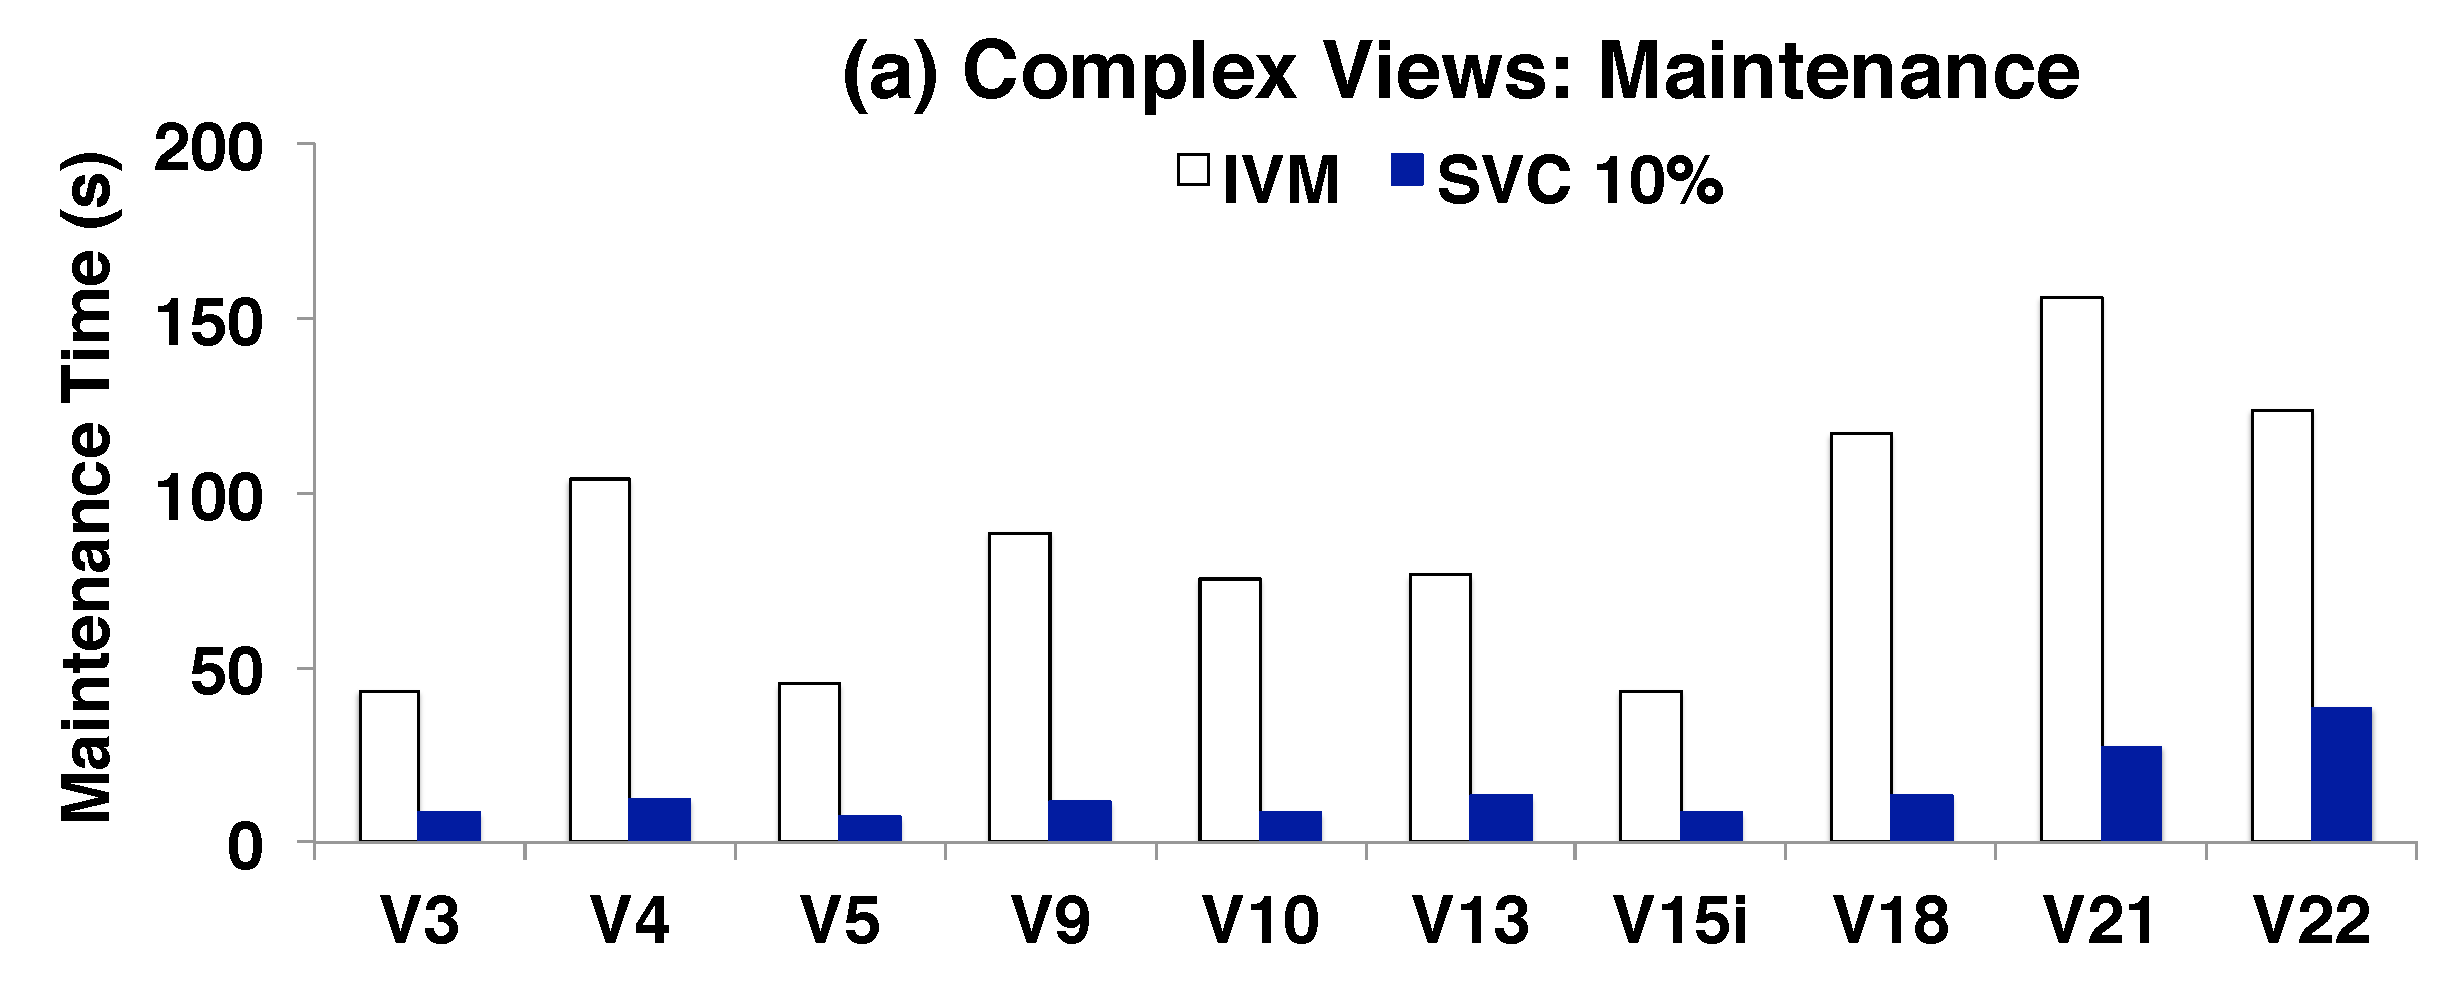
\includegraphics[scale=0.13]{exp/msqv_1.pdf}\vspace{.5em}
 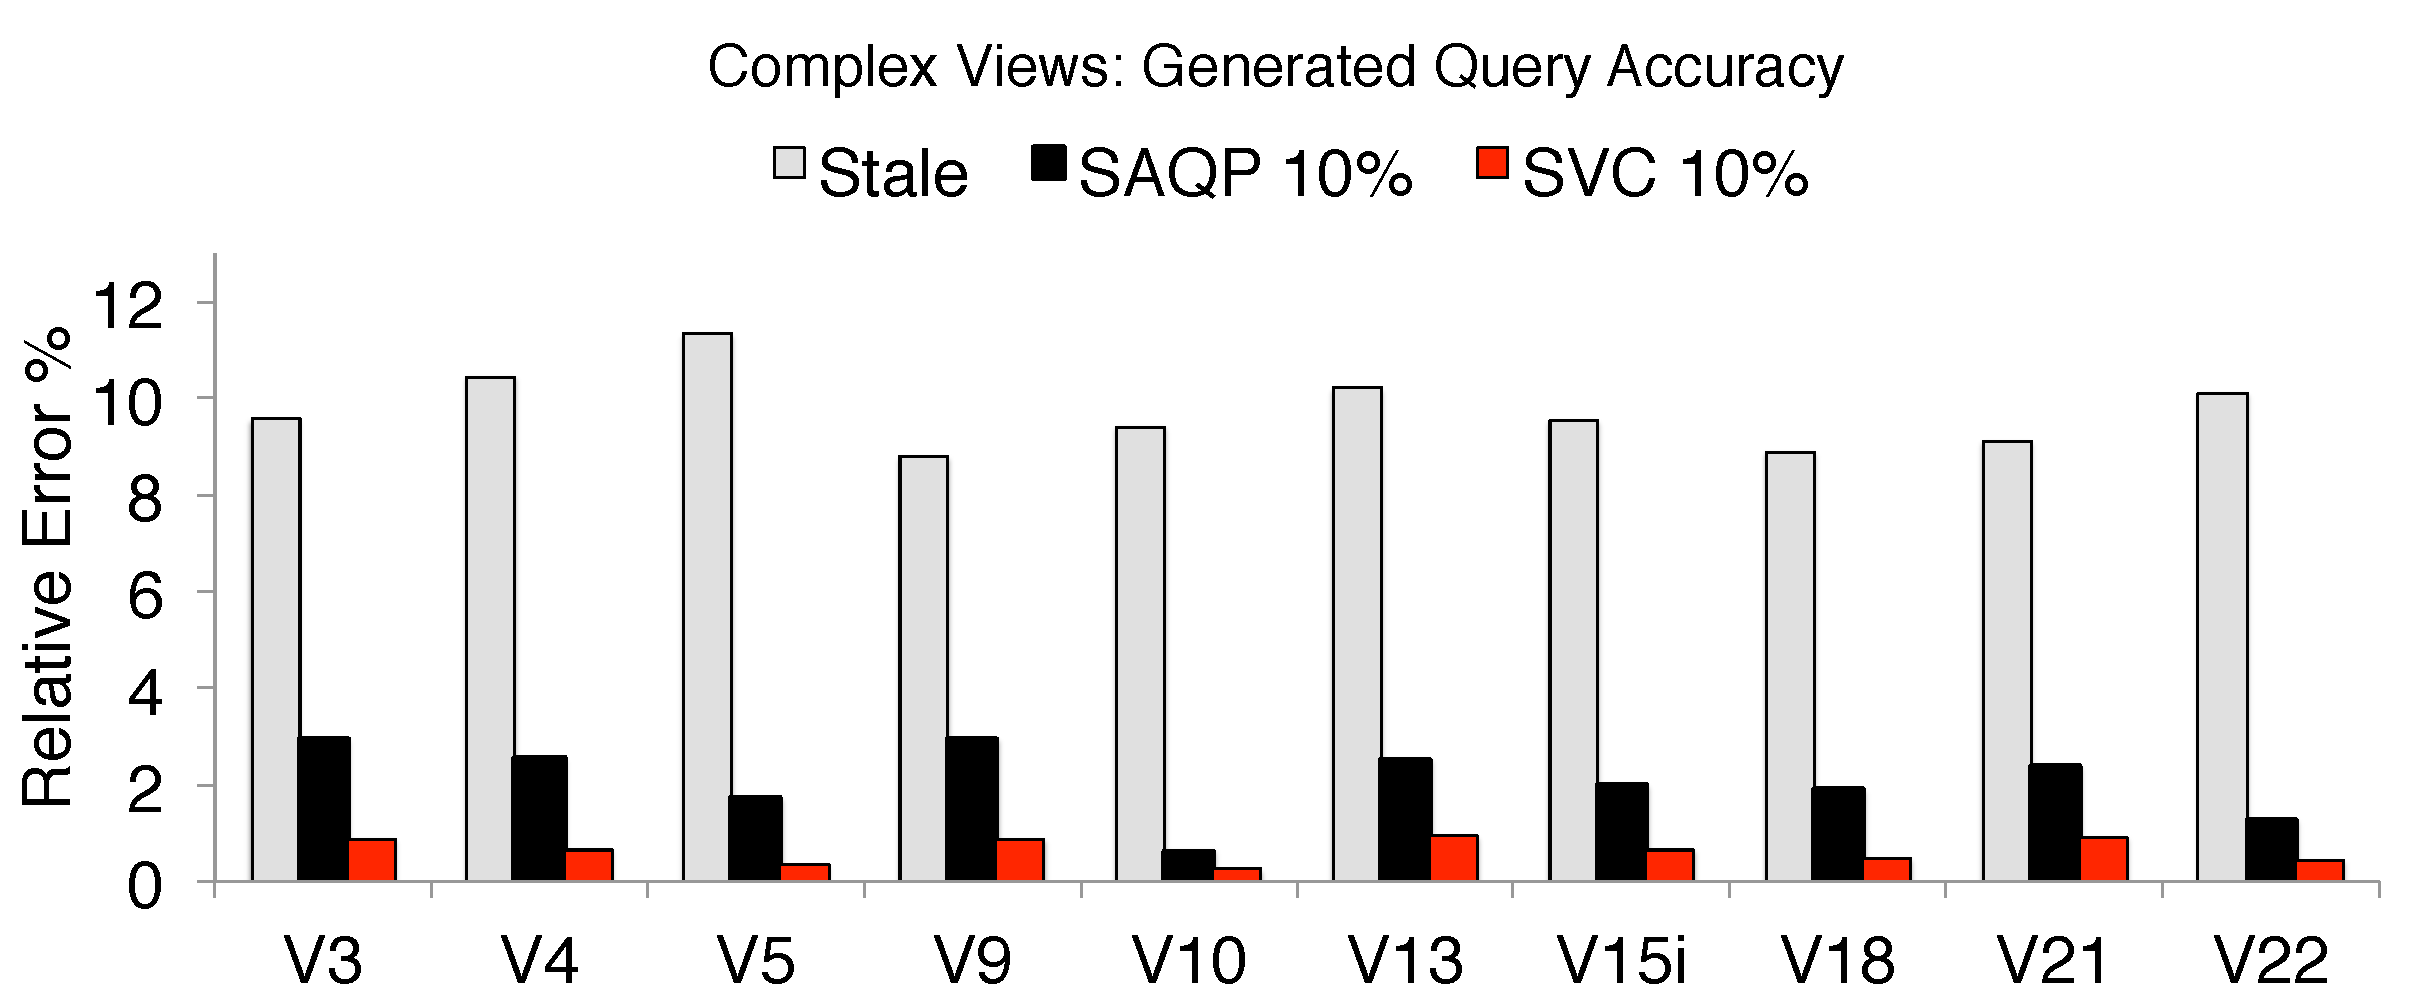
\includegraphics[scale=0.13]{exp/msqv_2.pdf} %\vspace{-1em}
 \caption{(a) For 1GB update size, we compare maintenance time and accuracy of \svc with a 10\% sample on different views. V21 and V22 do not benefit as much from \svc due to nested query structures. (b) As before for a 10\% sample size and 10\% update size, \svcnospace+Corr is more accurate than \svcnospace+AQP and No Maintenance.  \label{exp3-acc}}
\end{figure}
In this experiment, we demonstrate the breadth of views supported by \svc by using the TPCD queries as materialized views.
%Recall from our experiment description that each parameterized TPCD query is treated as a materialized view, and we use the \textsf{qgen} program 
%to generate 10 instances for each query.
%When we report results, we average over these 10 instances for each of the query types.

\textbf{Performance: }
Figure \ref{exp3-acc}, shows the maintenance time for a 10\% sample compared to the full view.
As before, we find that sampling saves a significant amount of maintenance time.
However, this experiment illustrates how the view definitions plays a role in the efficiency of our approach.
For the last two views, V21 and V22, we see that sampling does not lead to as large of speedup indicated in our previous experiments.  
This is because both of those views contain nested structures which block the pushdown of hashing.
V21 contains a subquery in its predicate that does not involve the primary key, but still requires a scan of the base relation to evaluate.
V22 contains a string transformation of a key blocking the push down.
There might be a way to derive an equivalent expression with joins that could be sampled more efficiently, and we will explore this in future work.
For the most part, these results are consistent with our previous experiments showing that \svc is faster than IVM and more accurate than \svcnospace+AQP and no maintenance.


\subsubsection{Outlier Indexing}

\begin{figure}[t] \vspace{-.5em}
\centering
 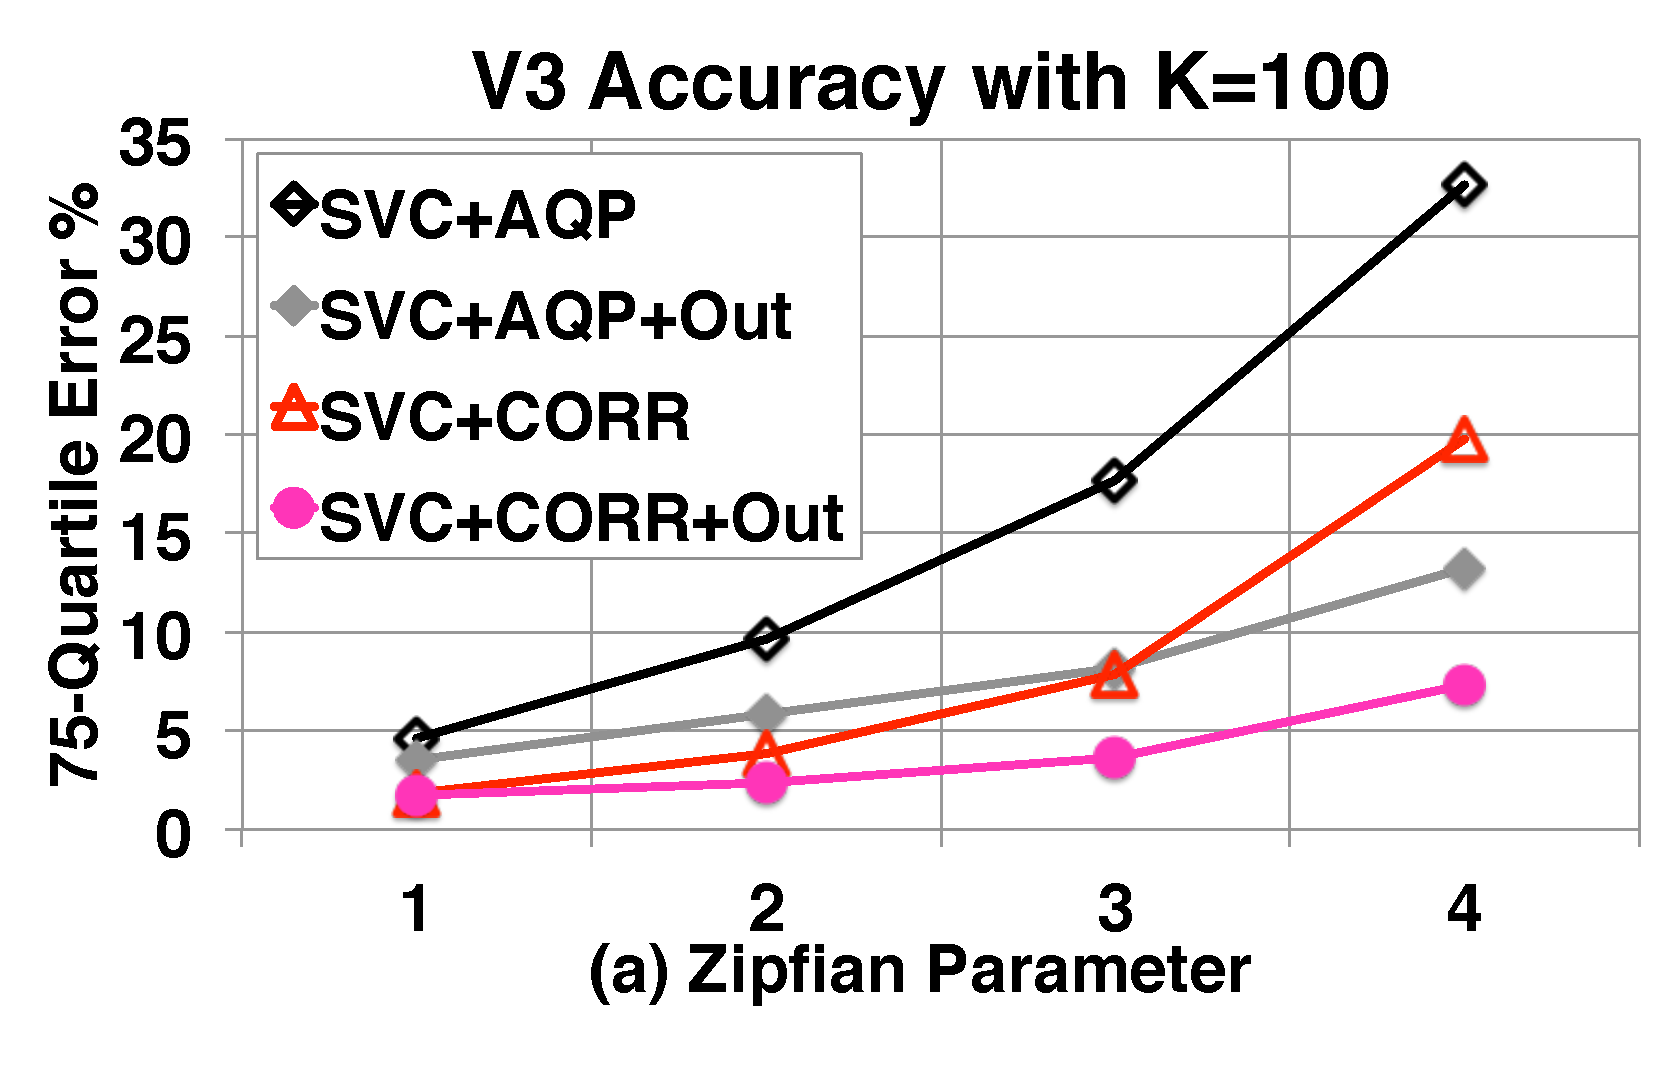
\includegraphics[scale=0.13]{exp/msoi_2.pdf}
 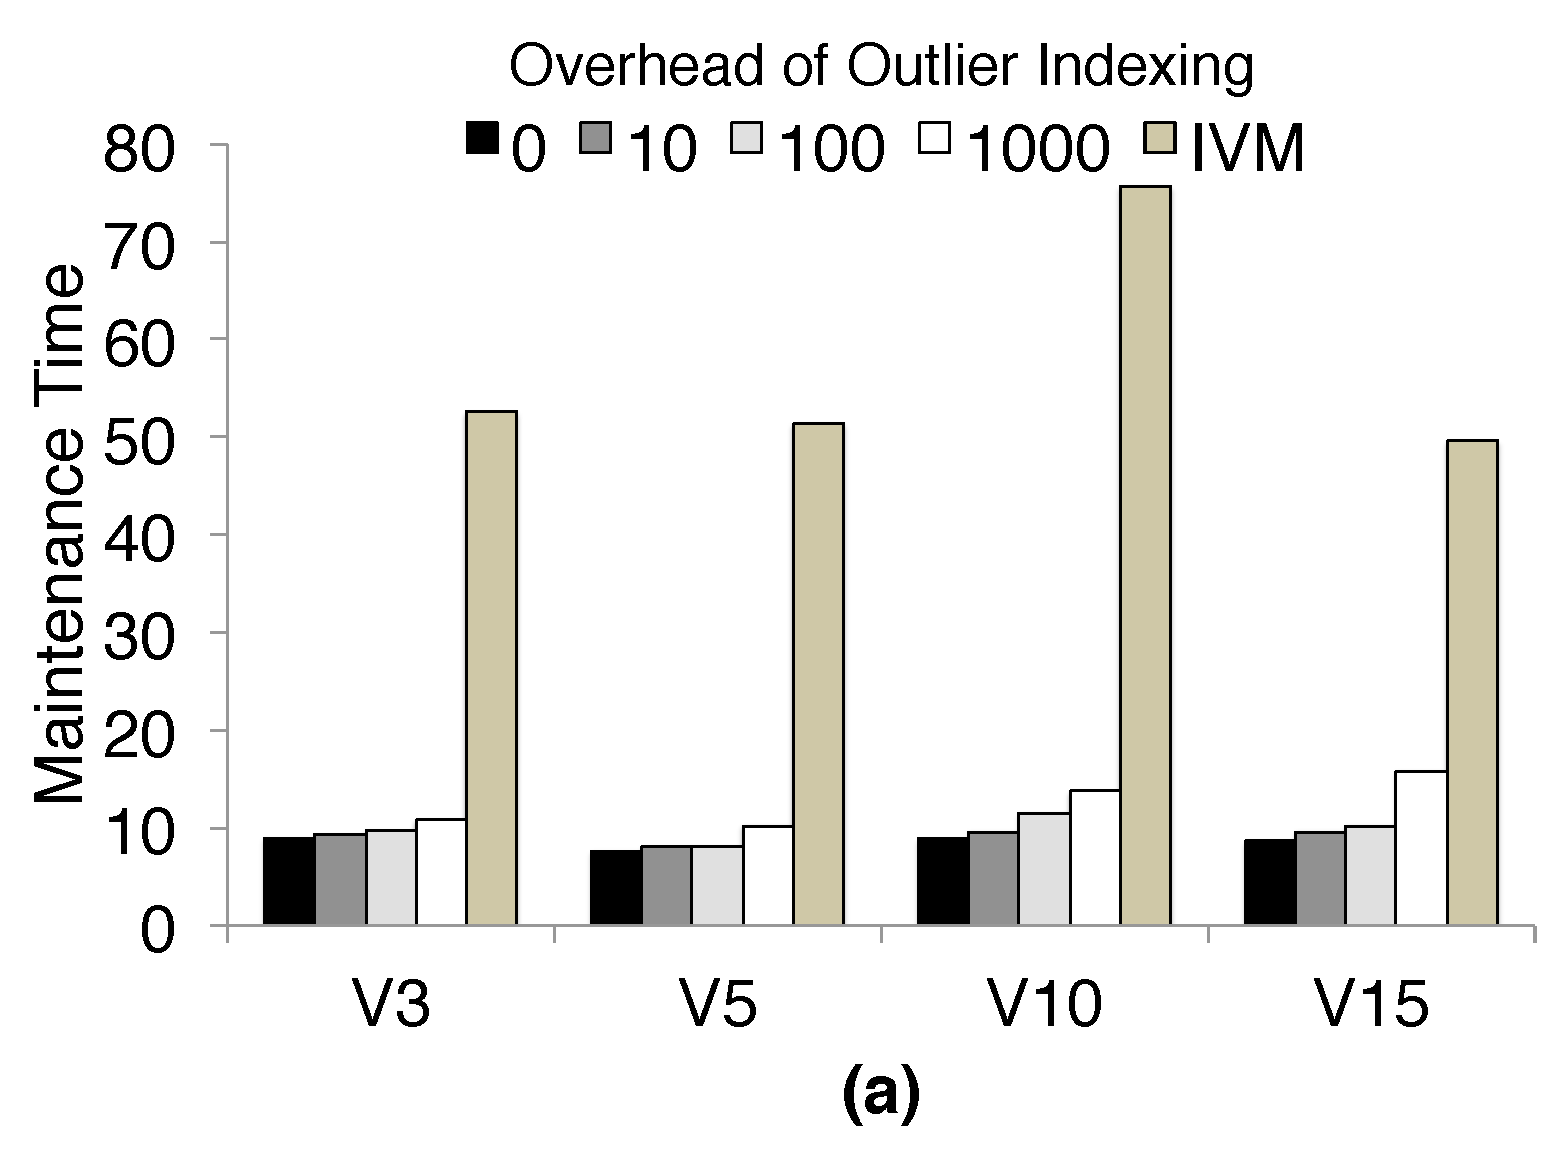
\includegraphics[scale=0.13]{exp/msoi_1.pdf}\vspace{-1em}
 \caption{(a) For one view V3 and 1GB of updates, we plot the 75\% quartile error with different techniques as we vary the skewness of the data. We find that \svc with an outlier index of size 100 is the most accurate. (b) While the outlier index adds an overhead this is small relative to the total maintenance time. \vspace{-1.5em}\label{exp5-oi}}
\end{figure}
In our next experiment, we evaluate our outlier indexing.
Our outlier indices are constructed on the base relations.
We index the \textsf{l\_extendedprice} attribute in the \textsf{lineitem} table.
We evaluate the outlier index on the complex TPCD views.
We find that four views: V3, V5, V10, V15, can benefit from this index with our push-up rules. 
These are four views dependent on \textsf{l\_extendedprice} that were also in the set of ``Complex'' views chosen before.

In our first outlier indexing experiment (Figure \ref{exp5-oi}(a)), we analyze V3.
We set an index of 100 records, and applied \svcnospace+Corr and \svcnospace+AQP to datasets with a skew parameter $z=\{1,2,3,4\}$. 
We run the same queries as before, but this time we measure the error at the 75\% quartile.
We find in the most skewed dataset \svc with outlier indexing reduces query error by a factor of 2.
Next, in \big(Figure \ref{exp5-oi} (b)\big), we plot the overhead for outlier indexing for V3 with an index size of 0, 10, 100, and 1000.
While there is an overhead, it is still small compared to the gains made by sampling the maintenance strategy.

\subsection{Conviva}
%In our next set of experiments, we applied \svc to a 1TB dataset of logs from Conviva.
%Recall, that we implement \svc on a 10-node Spark cluster. 
\subsubsection{Performance and Accuracy}
\begin{figure}[t] \vspace{-2em}
\centering
 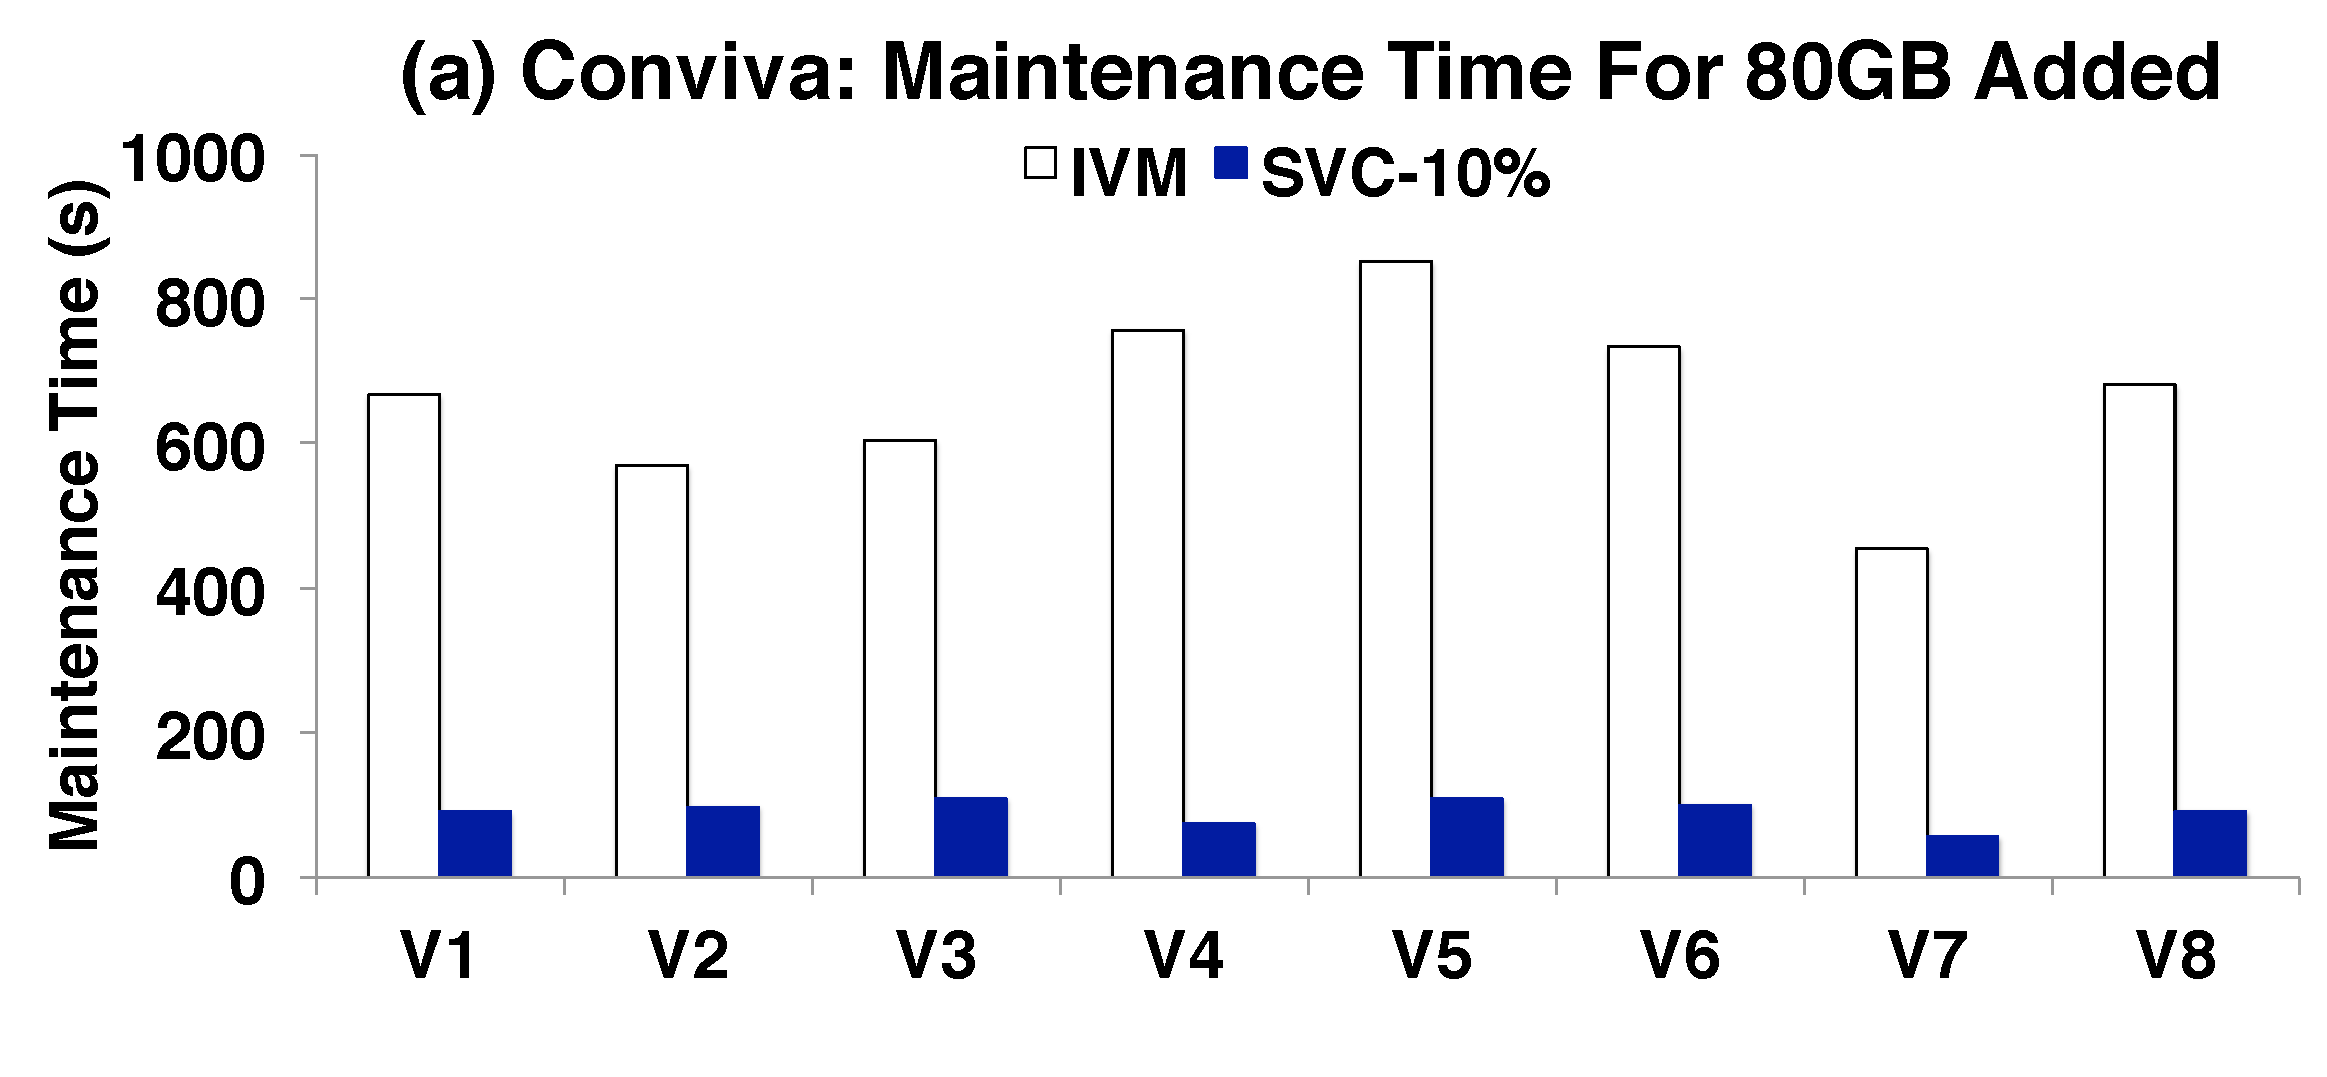
\includegraphics[scale=0.105]{exp/con_3.pdf}
 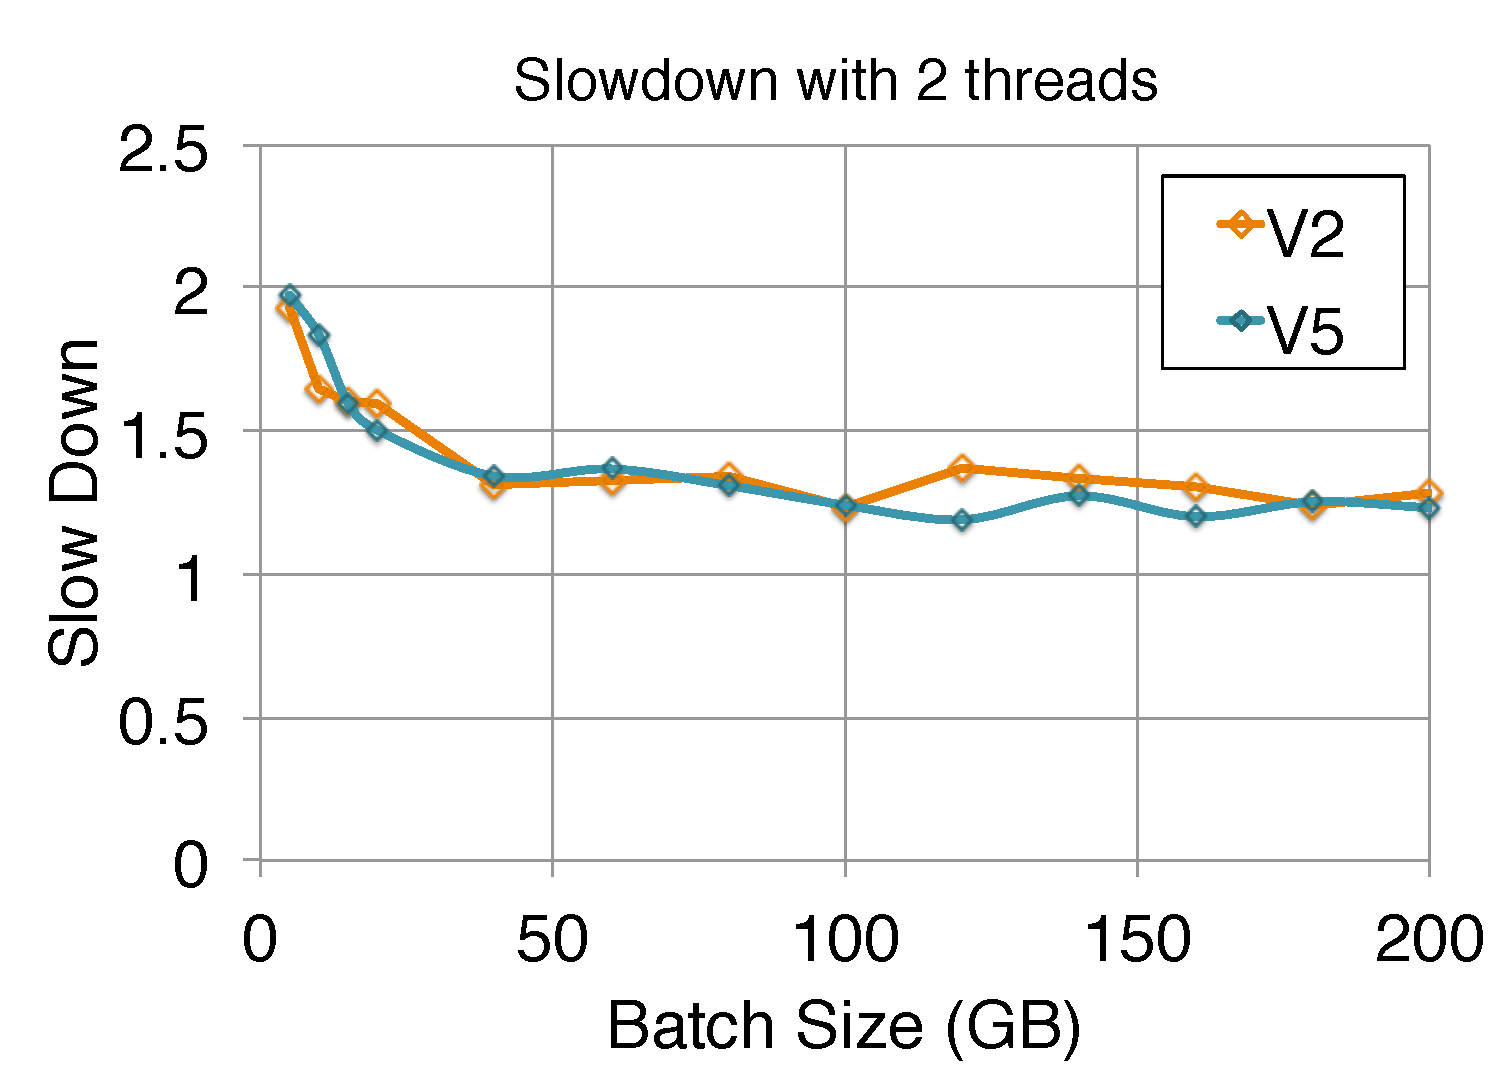
\includegraphics[scale=0.105]{exp/con_4.pdf} \vspace{-1.0em}
 \caption{(a) We compare the maintenance time of \svc with a 10\% sample and full incremental maintenance, and find that as with TPCD \svc saves significant maintenance time. (b) We also compare \svcnospace+Corr to \svcnospace+AQP and No Maintenance and find it is more accurate. \label{conv-1}}
\end{figure}
We derive the views from 800GB of base data and add 80GB of updates.
In Figure \ref{conv-1}(a), we show that while full maintenance takes nearly 800 seconds for one of the views, a \svc-10\% can complete sample maintenance in less than 100s for all of them.
On average over all the views, \svc-10\% gives a 7.5x speedup.

In Figure \ref{conv-1}(b), we show that \svc also gives highly accurate results with an average error of 0.98\%.
In the following experiments, we will use V2 and V5 as exemplary views.
V5 is the most expensive to maintain due to its nested query and V2 is a single level group by aggregate.
These results show consistency with our results on the synthetic datasets.

\subsubsection{End-to-end integration with periodic maintenance}
\begin{figure}[t]
\centering
 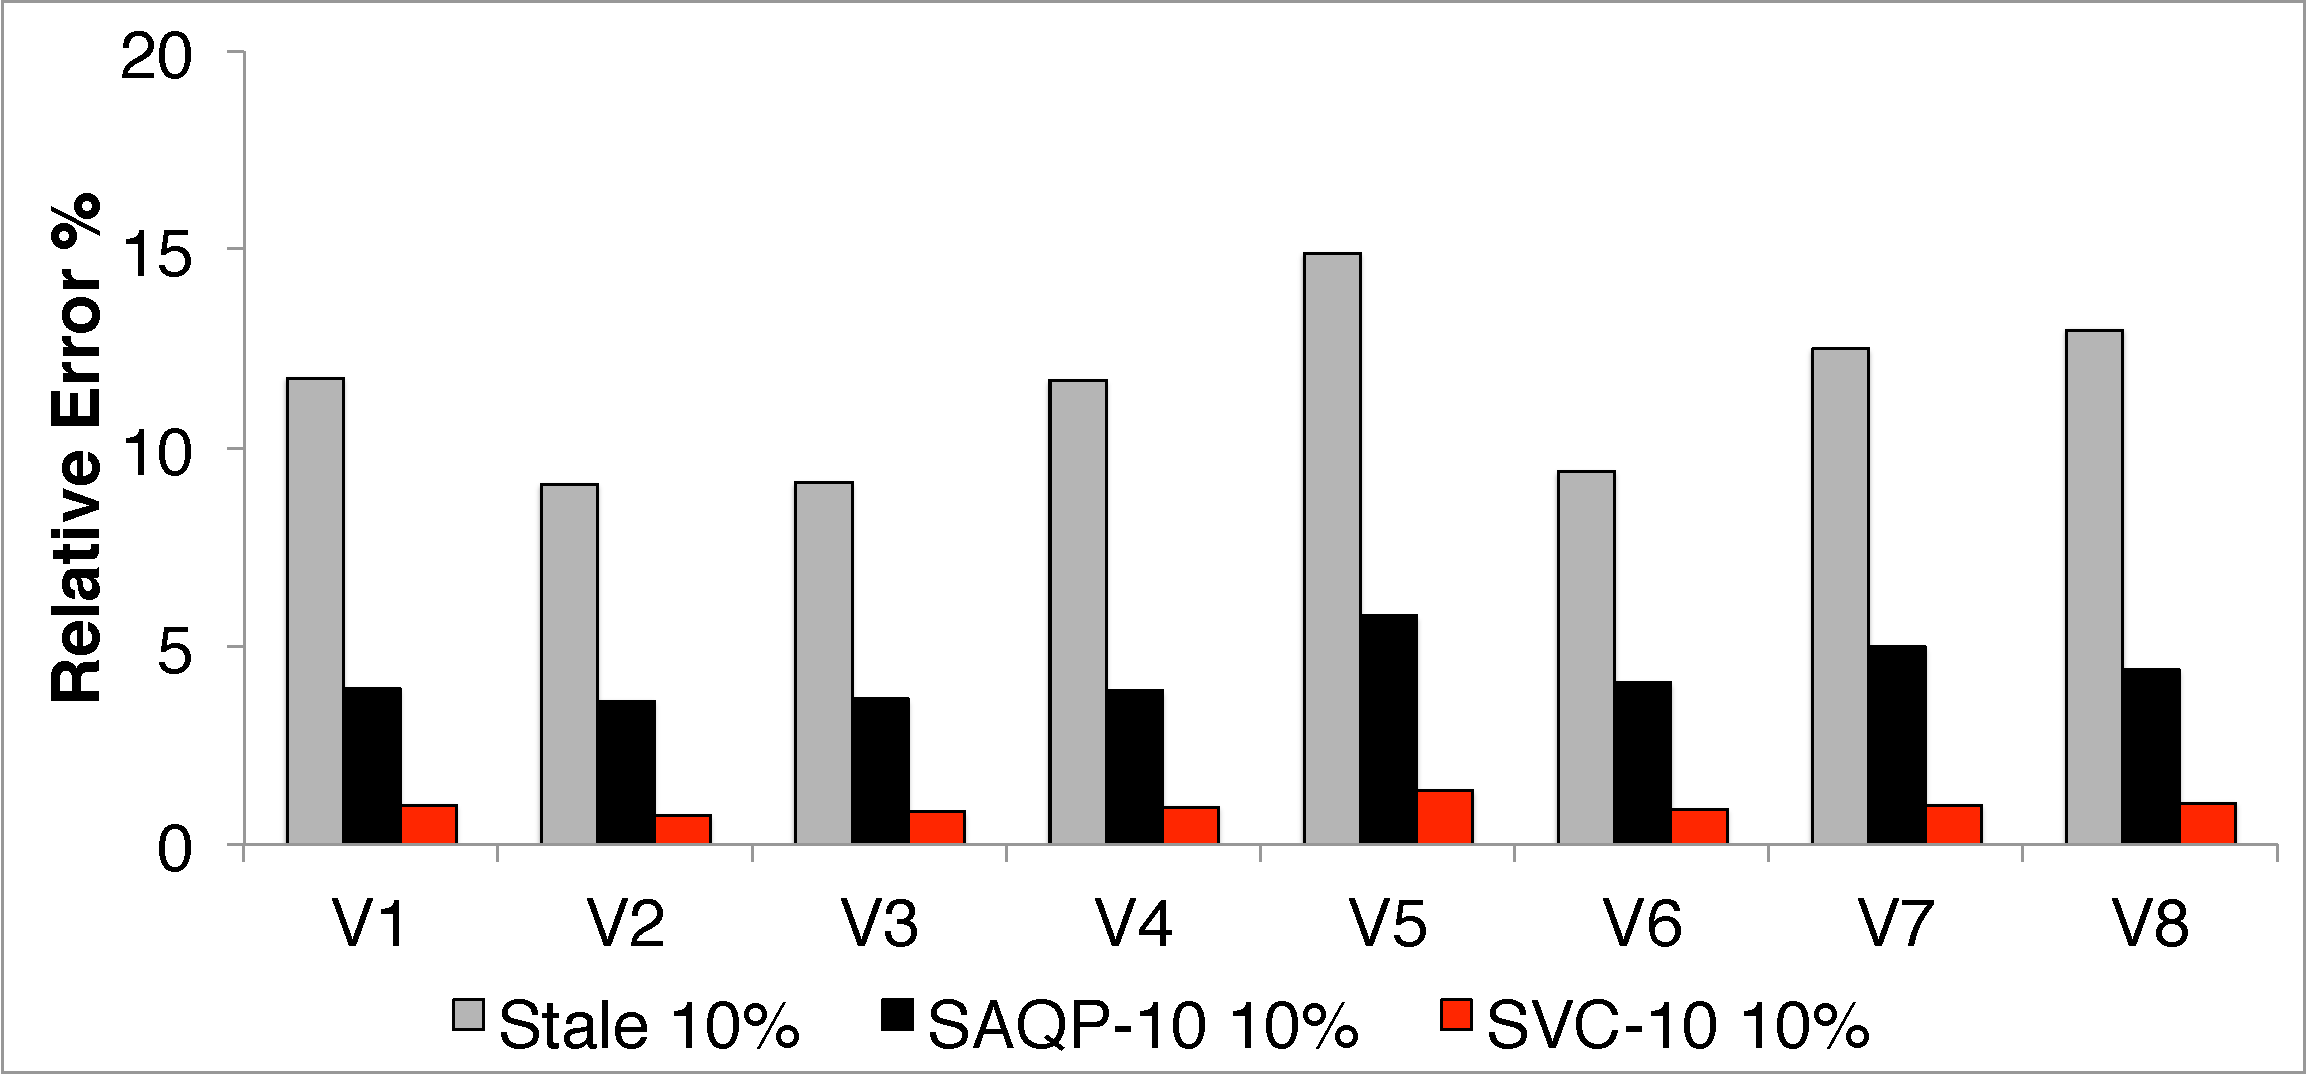
\includegraphics[scale=0.13]{exp/con_1.pdf}
 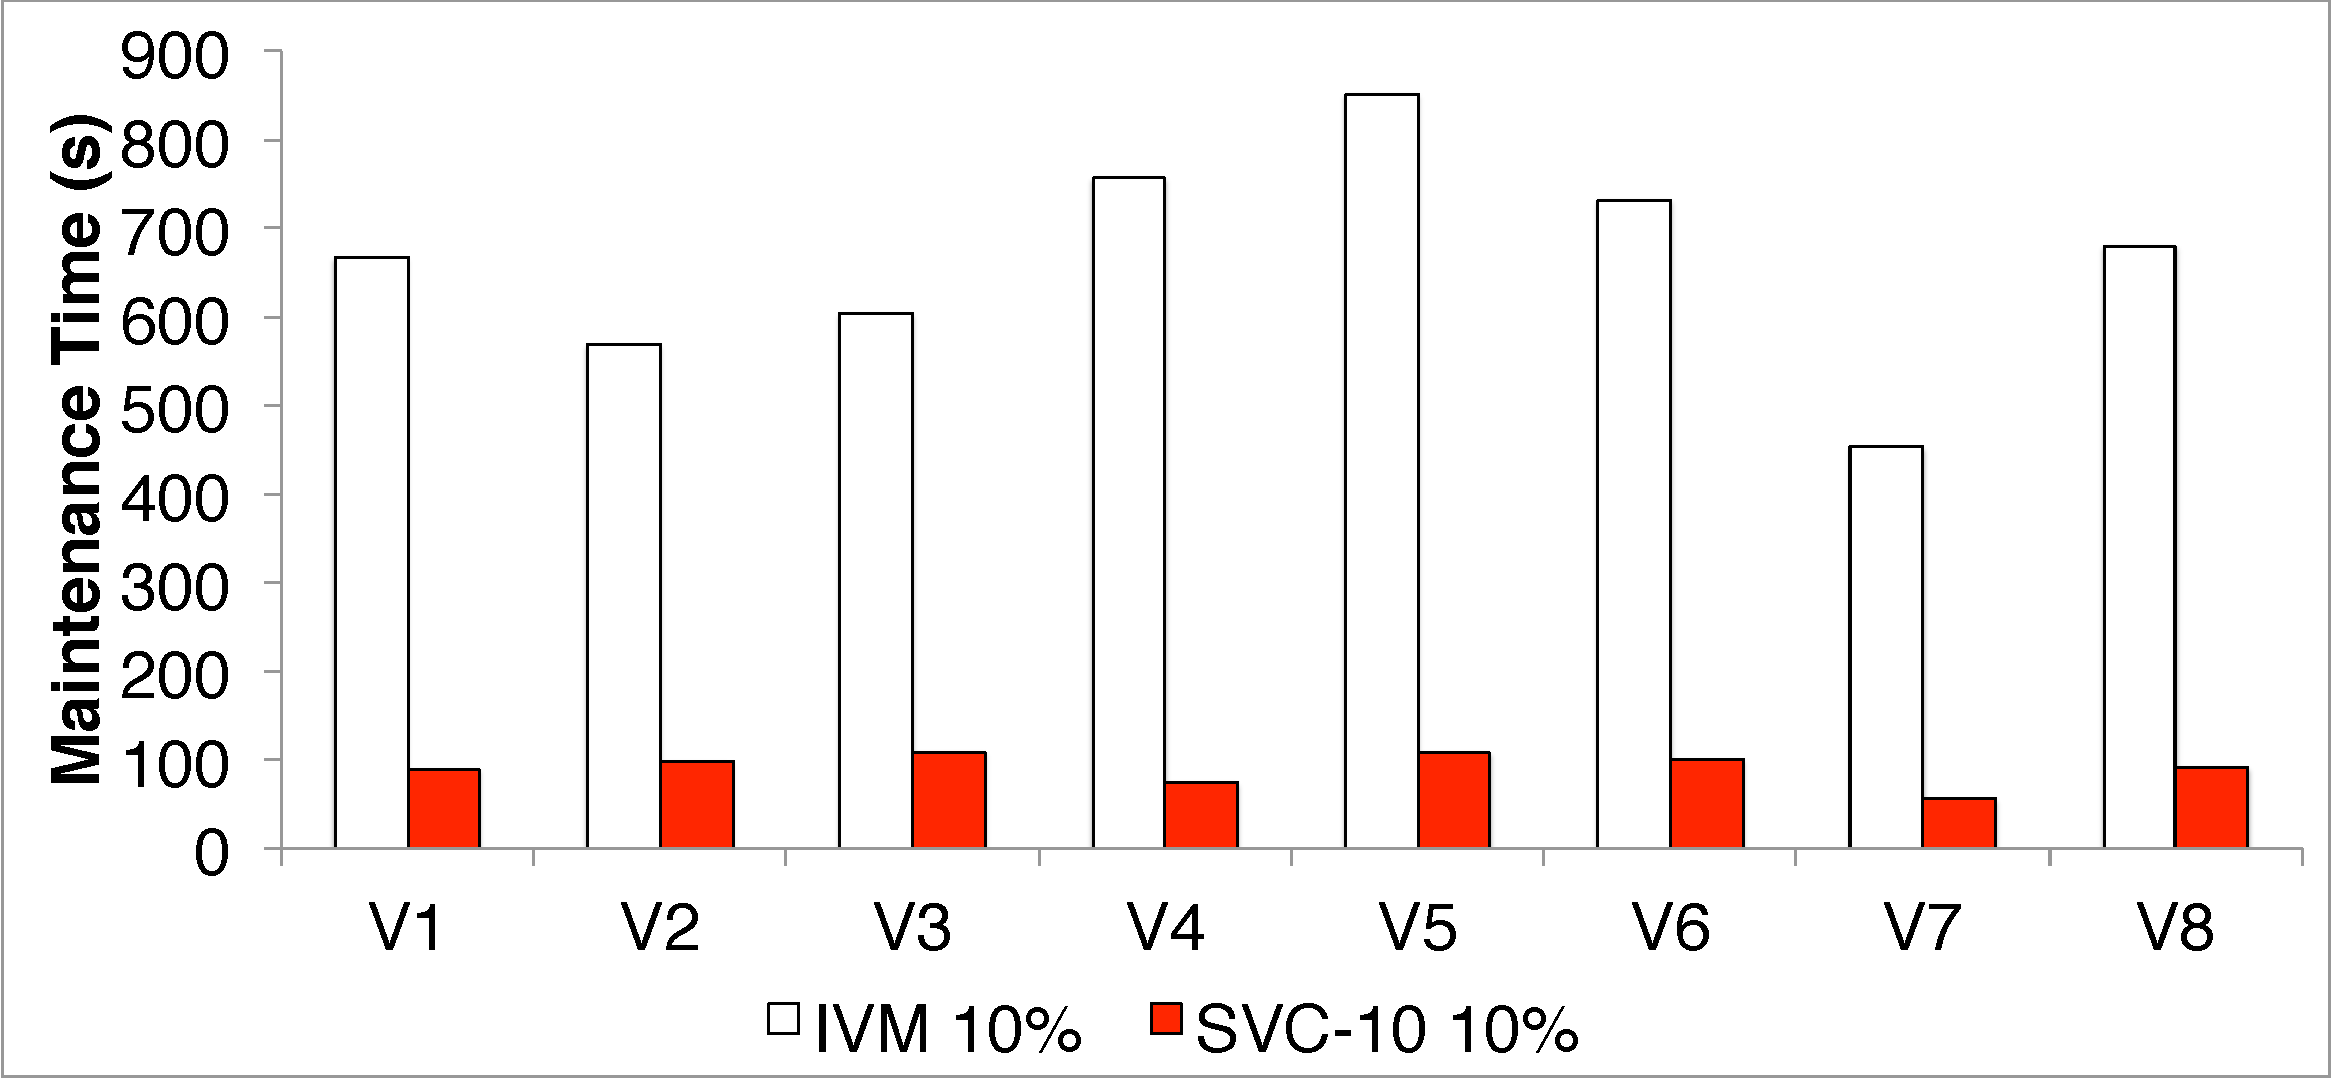
\includegraphics[scale=0.13]{exp/con_2.pdf}\vspace{-1em}
 \caption{(a) Spark RDDs are most efficient when updated in batches. As batch sizes increase the system throughput increases. (b) When running multiple threads, the throughput reduces. However, larger batches are less affected by this reduction. \label{conv-2}}\vspace{-1.25em}
\end{figure}

We devised an end-to-end experiment simulating a real integration with periodic maintenance.
However, unlike the MySQL case, Apache Spark does not support selective updates and insertions as the ``views'' are immutable.
A further point is that the immutability of these views and Spark's fault-tolerance requires that the ``views'' are maintained synchronously.
Thus, to avoid these significant overheads, we have to update these views in batches.
Spark does have a streaming variant \cite{zaharia2012discretized}, however, this does not support the complex SQL derived materialized views used in this paper, and still relies on mini-batch updates.

\svc and IVM will run in separate threads each with their own RDD materialized view.
In this application, both \svc and IVM maintain respective their RDDs with batch updates.
In this model, there are a lot of different parameters: batch size for periodic maintenance, batch size for \svc, sampling ratio for \svc, and the fact that concurrent threads may reduce overall throughput.
Our goal is to fix the throughput of the cluster, and then measure whether \svcnospace+IVM or IVM alone leads to more accurate query answers.

\textbf{Batch Sizes:} In Spark, larger batch sizes amortize overheads better.
In Figure \ref{conv-2}(a), we show a trade-off between batch size and throughput of Spark for V2 and V5.
Throughputs for small batches are nearly 10x smaller than the throughputs for the larger batches. 

\textbf{Concurrent \svc and IVM:} Next, we measure the reduction in throughput when running multiple threads.
We run \svc-10 in loop in one thread and IVM in another.
We measure the reduction in throughput for the cluster from the previous batch size experiment.
In Figure \ref{conv-2}(b), we plot the throughput against batch size when two maintenance threads are running.
While for small batch sizes the throughput of the cluster is reduced by nearly a factor of 2, for larger sizes the reduction is
smaller.
As we found in later experiments (Figure \ref{conv-5}), larger batch sizes are more amenable to parallel computation since there was more idle CPU time.


\textbf{Choosing a Batch Size:}
The results in Figure \ref{conv-2}(a) and Figure \ref{conv-2}(b) show that larger batch sizes are more efficient, however, larger batch sizes also lead to more staleness.
Combining the results in Figure \ref{conv-2}(a) and Figure \ref{conv-2}(b), for both \svcnospace+IVM and IVM, we get cluster throughput as a function of batch size.
For a fixed throughput, we want to find the smallest batch size that achieves that throughput for both.
For V2, we fixed this at 700,000 records/sec and for V5 this was 500,000 records/sec.
For IVM alone the smallest batch size that met this throughput demand was 40GB for both V2 and V5.
And for \svcnospace+IVM, the smallest batch size was 80GB for V2 and 100GB for V5. 
When running periodic maintenance alone view updates can be more frequent, and when run in conjunction with \svc it is less frequent. 

We run both of these approaches in a continuous loop, \svcnospace+IVM and IVM, and measure their maximal error during a maintenance period.
There is further a trade-off with the sampling ratio, larger samples give more accurate estimates however between \svc batches they go stale.
We quantify the error in these approaches with the max error; that is the maximum error in a maintenance period (Figure \ref{conv-4}).
These competing objective lead to an optimal sampling ratio of 3\% for V2 and 6\% for V5.
At this sampling point, we find that applying \svc gives results 2.8x more accurate for V2 and 2x more accurate for V5.

\begin{figure}[t]\vspace{-2em}
\centering
 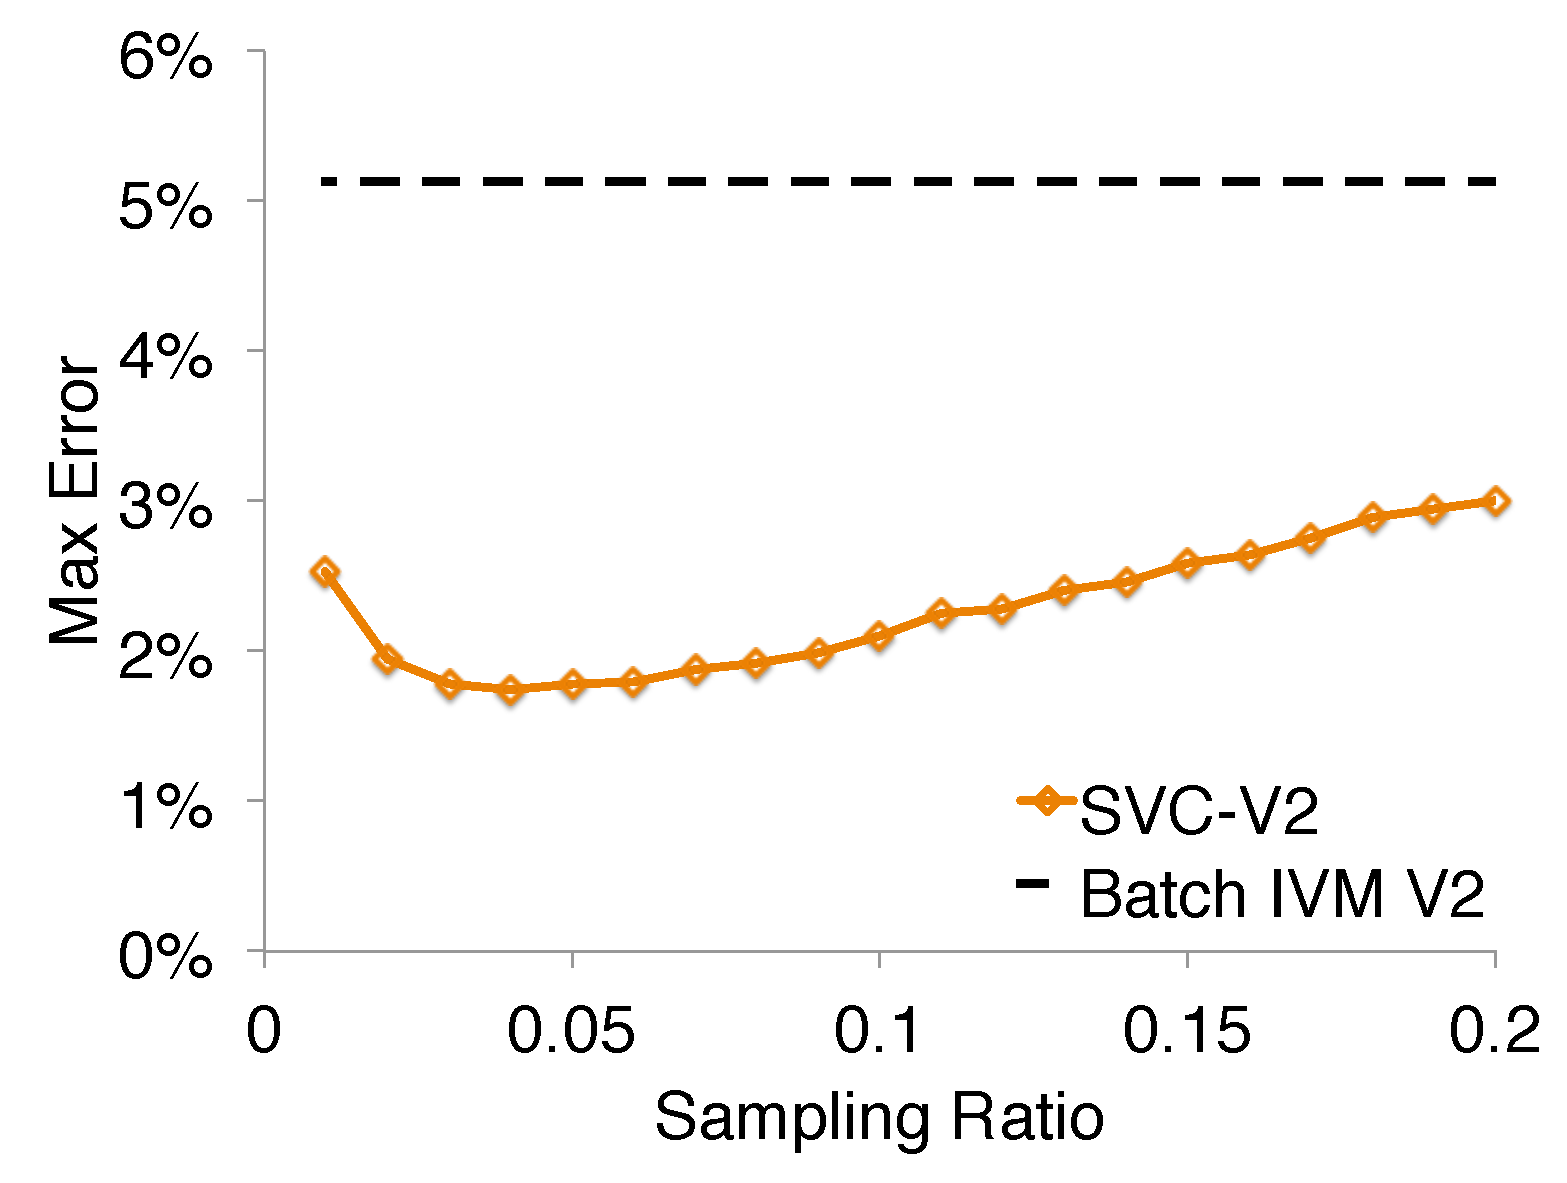
\includegraphics[scale=0.12]{exp/con_5.pdf}
 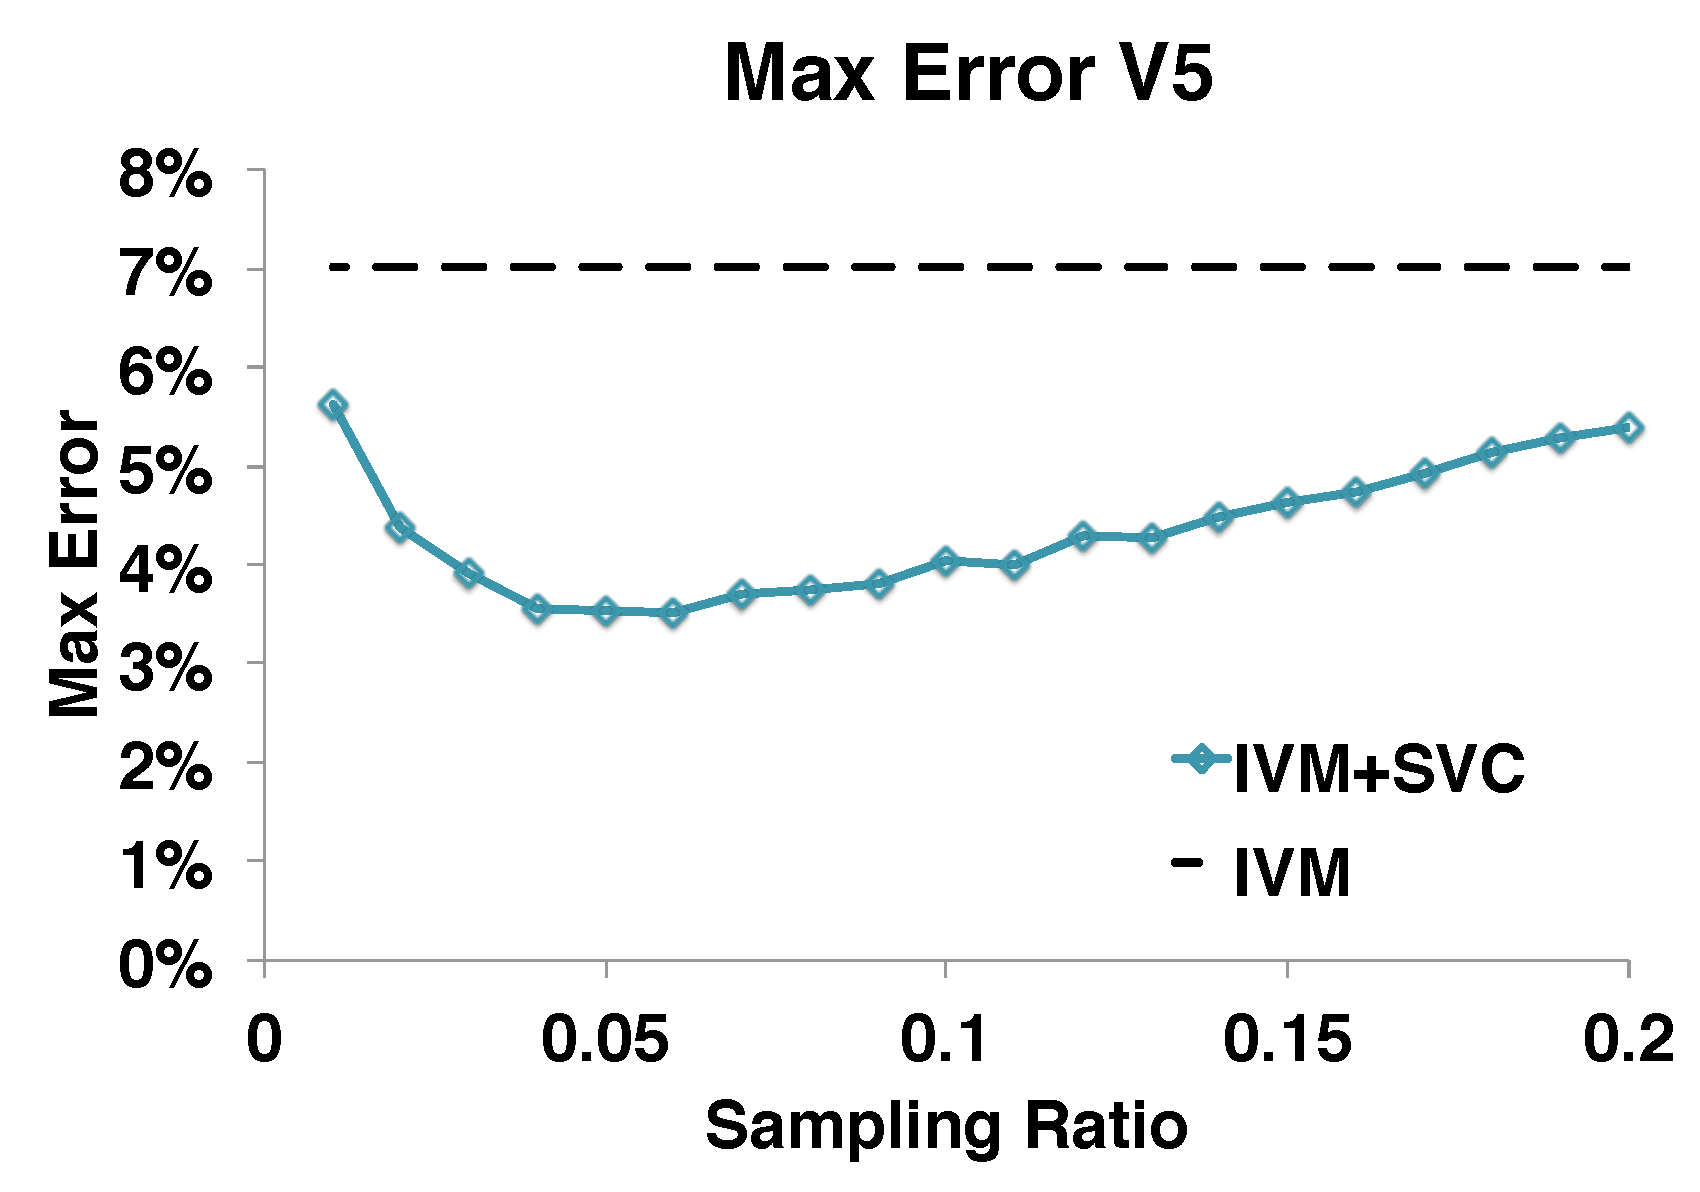
\includegraphics[scale=0.12]{exp/con_6.pdf}\vspace{-0.5em}
 \caption{For a fixed throughput, \svcnospace+Periodic Maintenance gives more accurate results for V2 and V5. \label{conv-4}} 
\end{figure}

\begin{figure}[t]
\centering
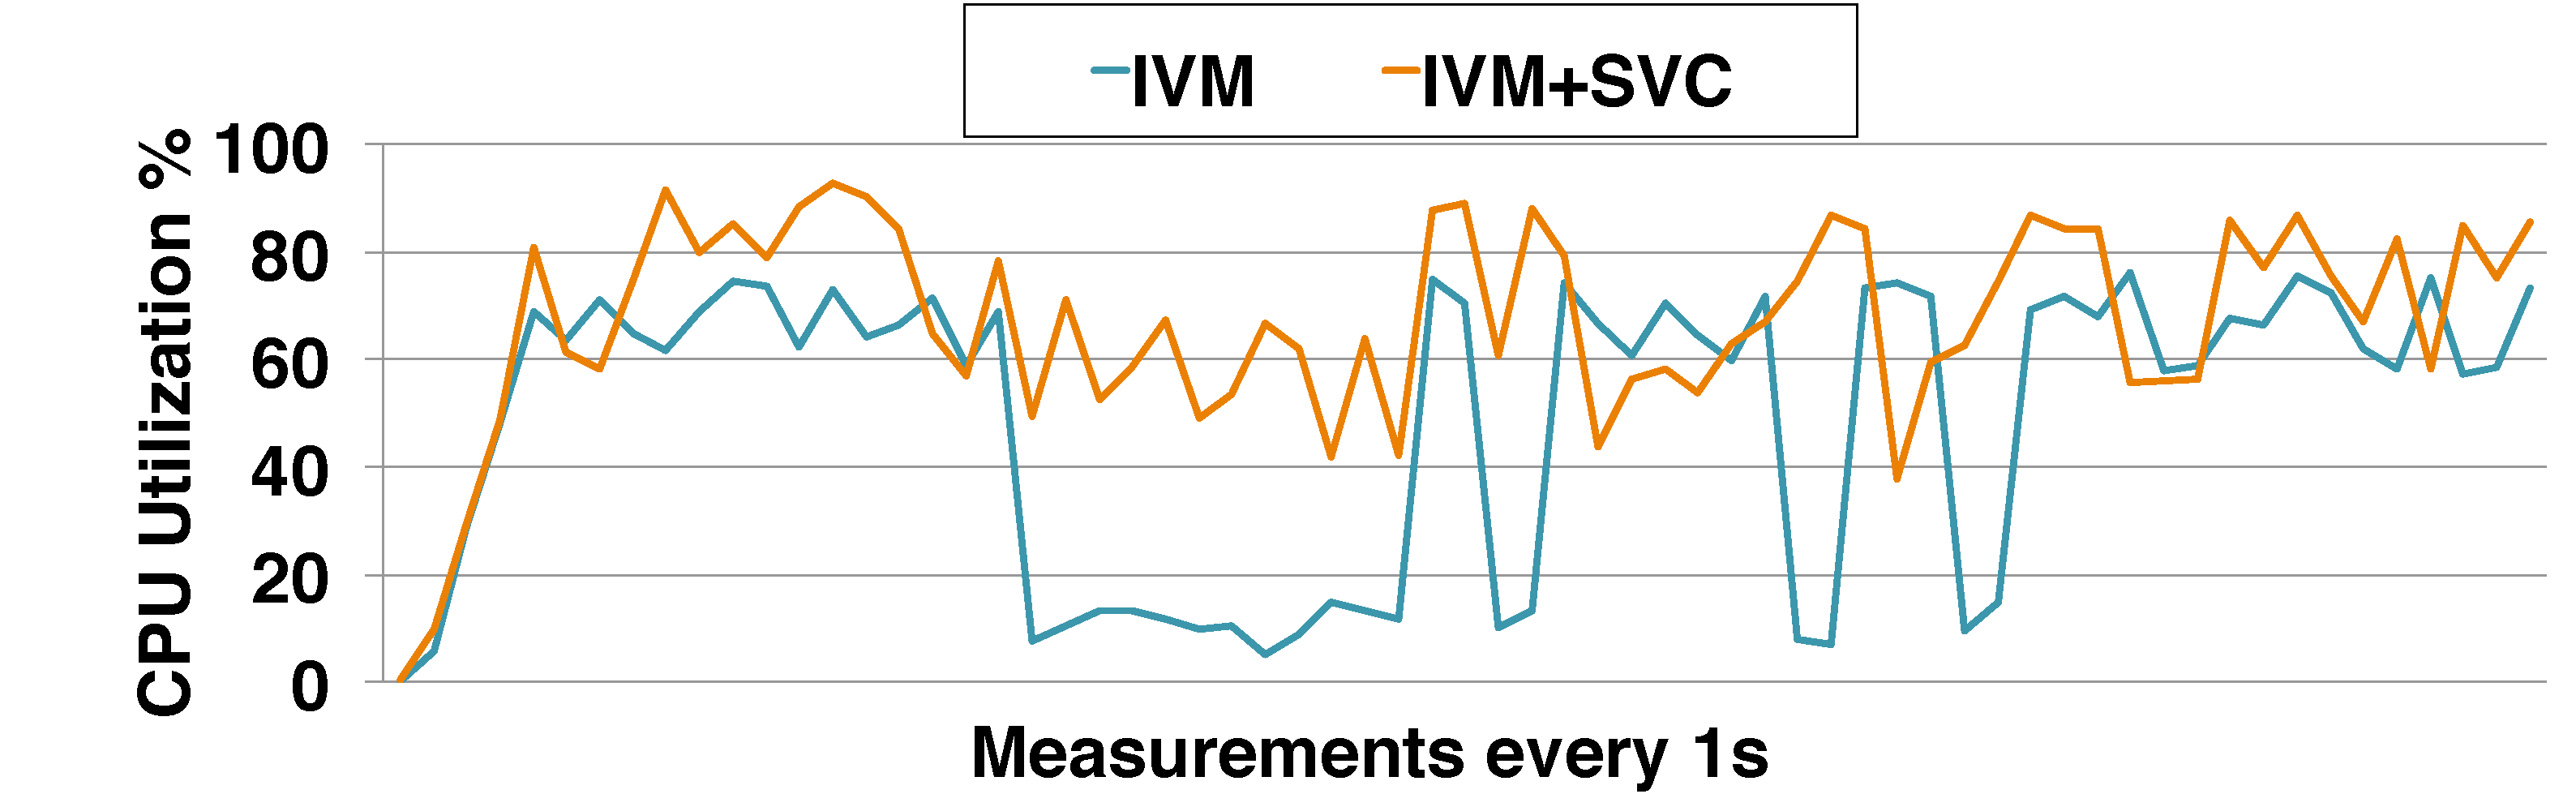
\includegraphics[scale=0.12]{exp/con_7.pdf}\vspace{-1em}
 \caption{\svc better utilizes idle times in the cluster by maintaining the sample.\label{conv-5}} \vspace{-1.5em}
\end{figure}

To give some intuition on why \svc gives more accurate results, in Figure \ref{conv-5}, we plot the average CPU utilization of the cluster for both periodic IVM and \svcnospace+periodic IVM. 
We find that \svc takes advantage of the idle times in the system; which are common during shuffle operations in a synchronous parallelism model.

In a way, these experiments present a worst-case application for \svc, yet it still gives improvements in terms of query accuracy.
In many typical deployments throughput demands are variable forcing maintenance periods to be longer, e.g., nightly.
The same way that \svc takes advantage of micro idle times during communication steps, it can provide large gains during controlled idle times when no maintenance is going on concurrently.




\vspace{-.75em}
\section{Related Work}\label{related}
\vspace{-.25em}
Addressing the cost of materialized view maintenance is the subject of many recent papers, which
focus on various perspectives including complex analytical queries~\cite{nikolic2014linview}, transactions~\cite{bailis2014scalable}, and physical design~\cite{lefevre2014opportunistic}.
The increased research focus parallels a major concern in industrial systems for incrementally updating pre-computed results and indices such as Google Percolator~\cite{percolator} and Twitter's Rainbird~\cite{rainbird}.
The streaming community has also studied the view maintenance problem \cite{abadi2003aurora,golab2011consistency, golab2012scalable, he2010comet, ghanem2010supporting, KrishnamurthyFDFGLT10}. In Spark Streaming, Zaharia et~al. studied how they could exploit in-memory materialization~\cite{zaharia2012discretized}, and in MonetDB, Liarou et~al. studied how ideas from columnar storage can be applied to enable real-time analytics \cite{liarou2012monetdb}.


Sampling has been well studied in the context of query processing~\cite{AgarwalMPMMS13, olken1993random, garofalakis2001approximate}. Particularly, a similar idea of sampling from updates has also been applied in stream processing~\cite{tatbul2003load, Garofalakis, rabkin2014aggregation}. But none of these works studied how to sample update patterns w.r.t materialized views and how to use the sample update patterns to correct stale query results.
%However, we argue, that our application of sampling in this work has a fundamentally different goal.
%Prior work emphasizes sampling as a technique to reduce query execution time.
%We, on the other hand, use sampling to reduce maintenance costs.
%This is similar to the goals of load shedding studied in streaming databases .
%Babcok et al. studied load shedding in the context of predefined aggregate queries, however, did not support ad hoc queries on the streaming data \cite{babcock2004load}.
Sampling has also been studied in the context of materialized views~\cite{joshi2008materialized,DBLP:conf/icde/OlkenR92}.
These techniques mirror what we called SAQP in our evaluation.
%Their focus, however, was not addressing incremental maintenance costs but rather operations on materialized views.
%They proposed a tree-like data structure that could support queries on multiple materialized views and operations on these views.
Gibbons et al. studied the maintenance of approximate histograms~\cite{gibbons1997fast}, which closely resemble aggregation materialized views.
They, however, did not consider queries on these histograms, but rather, they took a holistic approach to analyzing the error over the entire histogram.
Our approach differs from this work in that we do not estimate query results directly from a sample. 
Instead, we use samples to learn how updates affect the query results and then compensate for those differences. 
%We use the sample to learn how the updates affect the query results and then compensate for those changes.
Our experiments suggest that our approach is more accurate than SAQP when updates are sparse and the maintenance batch is small compared to the base data.

There are a variety of other efforts proposing storage efficient processing of aggregate queries on streams \cite{dobra2002processing, greenwald2001space} which are similar to materialized views. Furthermore, there is a close relationship between sampling and probabilistic databases, and view maintenance and selection in the context of probabilistic databases have also been studied \cite{re2007materialized}.
Srinivasan and Carey studied a problem related to query correction which they called compensation-based query processing \cite{srinivasanC92}.
This work was applied in the context of concurrency control and did not consider sampling or materialization.

\vspace{-1em}
\section{Conclusion and Future Work}\label{conclusion}
\vspace{-.3em}
In this paper, we propose a new approach to the staleness problem in materialized views.
We demonstrate how recent results from data cleaning, namely sampling, query correction, and outlier detection, can
allow for accurate query processing on stale views for a fraction of the cost of incremental maintenance. 
We evaluate this approach on a single node and in a distributed environment and find that SVC can correct stale query results 
with orders of magnitude less cost than full incremental maintenance.

Our results are promising and suggest many avenues for future work.
In particular, we are interested in deeper exploration of the multiple view setting.
Here, given a storage constraint and throughput demands, we can optimize sampling ratios over all views.
We are also interested in the possibility of sharing computation between materialized views and maintenance on views derived from other views.
We also believe there is a strong link between pre-computed machine learning models and materialized views, and the principles of our approach could be applied to build fast, approximate streaming machine learning applications.





\bibliographystyle{abbrv}
\fontsize{6.8pt}{6.7pt} \selectfont
\bibliographystyle{abbrv}
\bibliography{ref} 

\end{document}